\chapter{Synthetic Lethal Analysis of Gene Expression Data}
\label{chap:SLIPT}

\paragraph{Aims}

  \begin{itemize}
   \item Pathway Structure of Candidate Synthetic Lethal Genes for \textit{\textit{CDH1}} from TCGA breast data
   
   \bigskip
   
   \item Comparisons to Experimental siRNA Screen Candidates
   
   \bigskip
   
   \item Replication of Pathways across in TCGA Stomach data
  \end{itemize}

\paragraph{Summary}

    
  \begin{itemize}
   \item We have developed a Synthetic Lethal detection method that generates a high number of synthetic lethal candidates
   
   \bigskip
   
   \item Pathways in cell signalling, extracellular matrix, and cytoskeletal functions were supported with experimental candidates and the known functions of E-cadherin
   
   \bigskip
   
   \item Several candidate pathways were supported by mutation analysis and replicated across breast and stomach cancer
   
   \bigskip
   
   \item Translation and immune functions were uniquely detected by the computational approach which may be explained by differences between patient samples and cell line models
   
   \bigskip
   
   \item There remains the need to identify actionable genes within these pathways, relationships with experimental candidates, and how these pathways may affect viability when lost
  \end{itemize}


Having developed a statistical synthetic lethal detection methodology (SLIPT), it was applied to empirical (publicly avialable) cancer gene expression datasets in this chapter. The analysis largely focuses findings from the TCGA breast cancer data which covers a range of clinical subtypes and is more closely modelled by siRNA data \citep{Telford2015} generated from screening experiments conducted in MCF10A breast cells. Although stomach cancer data will also be considered to replicate findings in an independent dataset and for it's relevance to syndromic hereditary diffuse gastric cancer. The TCGA data also has the advantages of other clinical and molecular profiles (e.g., somatic mutation and DNA copy number) for many of the same samples, in addition to a considerable sample size for RNASeq expression data, treated with a rigourous procedure to minimise batch effects. Some findings will be replicated in the Cancer Cell Line Encyclopaedia which may be more comparable to the cell line experiments.

Synthetic lethal candidate partners for \textit{CDH1} will be described at both the gene and pathway level. SLIPT gene candidates will be analysed by cluster analysis for common expression profiles across samples and relationships with clinical factors and mutations in key breast cancer genes. These genes will also be compared to the gene candidates from a primary and secondary (validation) screens conducted by \citet{Telford2015} on isogenic cell lines. For comparison, an alternative SLIPT methodology which uses mutation data for \textit{CDH1} against expression of candidate partners will also be presented which may better represent the null mutations in HDGC patients and the experiment cell model \citep{Chen2014}. Pathways will be analysed by over-representation analysis (with resampling for comparisons with siRNA data) and supported by a metagene analysis of pathway gene signatures. The pathway metagene expression profiles will be used to replicate known relationships between clinical and molecular characteristics for breast cancer and to demonstrate application of SLIPT directly on metagenes to detect synthetic lethal pathways.

Together these results will demonstrate the wide range of applications for SLIPT analysis and examine the synthetic lethal partners of \textit{CDH1} in breast and stomach cancer. These synthetic lethal genes and pathways will be described in both context of the functional implications of novel synthetic lethal relationships and as potential actionable targets against \textit{CDH1} deficient tumours, in addition to replication of established functions of E-cadherin. In particular, the focus of these analysis will be in comparisons with experimental screening data to explore the potential for SLIPT to augment such triage of candidate partners and support further experimental investigations. The key synthetic lethal partner pathways for \textit{CDH1}, supported by both approaches, will be examined in more detail at the gene and pathway structure level in Chapter 5.

Some of the findings presented in this Chapter have also been included in manuscripts submitted for publication \citep{KellyHDGC, KellyBMC} and may bear similarity to them, although the results in this thesis have been edited to cohesively fit with additional findings. These findings are the result of investigations conducted throughout this thesis project and only these contributions to the articles are included in this chapter, not that conducted by co-authors.

\section{Synthetic lethal genes in breast cancer}

\begin{itemize}
 \item exprSL
 \item mtSL
 \item heatmap
\end{itemize}

The SLIPT methodology (as described in section \ref{methods:SLIPT}) was applied to the normalised TCGA breast cancer gene expression dataset ($n = 1168$). As shown in Table \ref{tab:gene_SL}, the most significant genes had strong evidence of expression-based association with \textit{CDH1} (high $\chi^2$ values) with fewer samples exhibiting low expression of both genes than expected statistically. Eukaryotic translation gene were among the highest gene candidates, including initiation factors, elongation factors, and ribosomal proteins. These are clearly neccessary for cancer cells to grow and proliferate, with sustained gene expression needed to maintain growth signaling pathways and resist apoptosis or immune factors translation may be subject to non-oncogene addiction for \textit{CDH1}-deficient cells.

While these are among the strongest synthetic lethal candidates, translational genes are cruicial to the viability of healthy cells and dosing for a selective synthetic lethal effect against these may be difficult compared to other biological functions which may also be supported among the SLIPT candidate genes. Furthermore, few known biological functions of \textit{CDH1} were among the strongest SL candidates so the remaining candidate genes may also be informative since they are likely to contain these expected functions in addition to novel relationships for \textit{CDH1}. Thus further pathway level analyses were also conducted to examine biological functions over-represent\-ed among synthetic candidate genes and identify synthetic lethal pathways.

\begin{table*}[!ht]
\caption{Candidate synthetic lethal genes against E-cadherin from SLIPT}
\label{tab:gene_SL}
\centering
\resizebox{0.8 \textwidth}{!}{
\begin{threeparttable}
\begin{tabular}{>{\em}sl^c^c^c^c^c}
\rowstyle{\bfseries}
 \em{Gene} & Observed & Expected & $\chi^2$ value & p-value & p-value (FDR) \\ 
  \hline
  \rowcolor{black!10}
TRIP10 & 62 & 130 & 162 & $5.65 \times 10^{-34}$ & $1.84 \times 10^{-31}$ \\
  \rowcolor{black!5} 
  EEF1B2 & 56 & 130 & 158 & $3.10 \times 10^{-33}$ & $9.45 \times 10^{-31}$ \\
  \rowcolor{black!10} 
  GBGT1 & 61 & 131 & 156 & $1.08 \times 10^{-32}$ & $3.14 \times 10^{-30}$ \\
  \rowcolor{black!5} 
  ELN & 81 & 130 & 149 & $3.46 \times 10^{-31}$ & $8.82 \times 10^{-29}$ \\
  \rowcolor{black!10} 
  TSPAN4 & 78 & 130 & 146 & $1.63 \times 10^{-30}$ & $3.79 \times 10^{-28}$ \\
  \rowcolor{black!5} 
  GLIPR2 & 72 & 130 & 146 & $1.68 \times 10^{-30}$ & $3.86 \times 10^{-28}$ \\
  \rowcolor{black!10} 
  RPS20 & 73 & 131 & 145 & $1.89 \times 10^{-30}$ & $4.28 \times 10^{-28}$ \\
  \rowcolor{black!5} 
  RPS27A & 80 & 130 & 143 & $5.53 \times 10^{-30}$ & $1.18 \times 10^{-27}$ \\
  \rowcolor{black!10} 
  EEF1A1P9 & 63 & 130 & 141 & $1.91 \times 10^{-29}$ & $3.74 \times 10^{-27}$ \\
  \rowcolor{black!5} 
  C1R & 73 & 130 & 141 & $2.05 \times 10^{-29}$ & $3.97 \times 10^{-27}$ \\
  \rowcolor{black!10} 
  LYL1 & 73 & 130 & 140 & $2.99 \times 10^{-29}$ & $5.74 \times 10^{-27}$ \\
  \rowcolor{black!5} 
  RPLP2 & 71 & 130 & 139 & $4.88 \times 10^{-29}$ & $9.07 \times 10^{-27}$ \\
  \rowcolor{black!10} 
  C10orf10 & 73 & 130 & 138 & $6.72 \times 10^{-29}$ & $1.20 \times 10^{-26}$ \\
  \rowcolor{black!5} 
  DULLARD & 74 & 131 & 138 & $9.29 \times 10^{-29}$ & $1.61 \times 10^{-26}$ \\
  \rowcolor{black!10} 
  PPM1F & 64 & 130 & 136 & $1.61 \times 10^{-28}$ & $2.65 \times 10^{-26}$ \\
  \rowcolor{black!5} 
  OBFC2A & 69 & 130 & 136 & $2.49 \times 10^{-28}$ & $3.93 \times 10^{-26}$ \\
  \rowcolor{black!10} 
  RPL11 & 70 & 130 & 136 & $2.56 \times 10^{-28}$ & $3.97 \times 10^{-26}$ \\
  \rowcolor{black!5} 
  RPL18A & 70 & 130 & 135 & $3.08 \times 10^{-28}$ & $4.70 \times 10^{-26}$ \\
  \rowcolor{black!10} 
  MFNG & 76 & 131 & 133 & $7.73 \times 10^{-28}$ & $1.12 \times 10^{-25}$ \\
  \rowcolor{black!5} 
  RPS17 & 77 & 131 & 133 & $8.94 \times 10^{-28}$ & $1.29 \times 10^{-25}$ \\
  \rowcolor{black!10} 
  MGAT1 & 73 & 130 & 132 & $1.44 \times 10^{-27}$ & $2.03 \times 10^{-25}$ \\
  \rowcolor{black!5} 
  RPS12 & 72 & 130 & 128 & $8.57 \times 10^{-27}$ & $1.12 \times 10^{-24}$ \\
  \rowcolor{black!10} 
  C10orf54 & 73 & 130 & 127 & $1.37 \times 10^{-26}$ & $1.75 \times 10^{-24}$ \\
  \rowcolor{black!5} 
  LOC286367 & 72 & 130 & 126 & $2.20 \times 10^{-26}$ & $2.70 \times 10^{-24}$ \\
  \rowcolor{black!10} 
  GMFG & 70 & 130 & 126 & $2.20 \times 10^{-26}$ & $2.70 \times 10^{-24}$ \\ 
  \hline
\end{tabular}
\begin{tablenotes}
\raggedright \small
Strongest candidate SL partners for \textit{CDH1} by SLIPT with observed and expected samples with low expression of both genes
\end{tablenotes}
\end{threeparttable}
}
\end{table*}

The modified mtSLIPT methodology (as described in section \ref{methods:SLIPT}) was also applied to the normalised TCGA breast cancer gene expression dataset, against somatic loss of function mutations in \textit{CDH1}. As shown in Table \ref{tab:gene_mtSL}, the most significant genes also had strong evidence of expression associated with \textit{CDH1} mutations (high $\chi^2$ values) with fewer samples exhibiting both low expression and mutations of each gene than expected statistically. Although, these were not a strongly supported as the expression analysis (in Table \ref{tab:gene_SL}) nor were as many genes detected. This is unsurprising due to the lower sample size with matching somatic mutation data and the lower frequency of \textit{CDH1} mutations compared to low expression by $\sfrac{1}{3}$ quantiles.

The mtSLIPT candidates had more genes involved in cell and gene regulation, particularly DNA and RNA binding factors. The strongest candidates also include microtubule (\textit{KIF12}), microfibril (\textit{MFAP4}), and cell adhesion (\textit{TENC1}) genes consistent with the established cytoskeletal role of \textit{CDH1}. The elastin gene (\textit{ELN}) was notably strongly supported by both expression and mutation SLIPT analysis of \text{CDH1} supporting a interactions with extracellular proteins and the tumour microenvironment.

\begin{table*}[!ht]
\caption{Candidate synthetic lethal genes against E-cadherin from mtSLIPT}
\label{tab:gene_mtSL}
\centering
\resizebox{0.8 \textwidth}{!}{
\begin{threeparttable}
\begin{tabular}{>{\em}sl^c^c^c^c^c}
\rowstyle{\bfseries}
 \em{Gene} & Observed & Expected & $\chi^2$ value & p-value & p-value (FDR) \\ 
  \hline
  \rowcolor{black!10}
TFAP2B & 8 & 36.7 & 89.5 & $3.60 \times 10^{-20}$ & $8.37 \times 10^{-17}$ \\
  \rowcolor{black!5}
  ZNF423 & 15 & 36.7 & 78.8 & $7.89 \times 10^{-18}$ & $1.22 \times 10^{-14}$ \\ 
  \rowcolor{black!10}
  CALCOCO1 & 11 & 36.7 & 76.8 & $2.09 \times 10^{-17}$ & $2.59 \times 10^{-14}$ \\ 
  \rowcolor{black!5}
  RBM5 & 13 & 36.7 & 75.7 & $3.65 \times 10^{-17}$ & $4.00 \times 10^{-14}$ \\ 
  \rowcolor{black!10}
  BTG2 & 7 & 36.7 & 71.7 & $2.72 \times 10^{-16}$ & $1.81 \times 10^{-13}$ \\ 
  \rowcolor{black!5}
  RXRA & 6 & 36.7 & 70.5 & $5.00 \times 10^{-16}$ & $2.97 \times 10^{-13}$ \\ 
  \rowcolor{black!10}
  SLC27A1 & 11 & 36.7 & 70.3 & $5.42 \times 10^{-16}$ & $2.97 \times 10^{-13}$ \\ 
  \rowcolor{black!5}
  MEF2D & 12 & 36.7 & 69.6 & $7.86 \times 10^{-16}$ & $3.95 \times 10^{-13}$ \\ 
  \rowcolor{black!10}
  NISCH & 12 & 36.7 & 69.6 & $7.86 \times 10^{-16}$ & $3.95 \times 10^{-13}$ \\ 
  \rowcolor{black!5}
  AVPR2 & 9 & 36.7 & 69.2 & $9.36 \times 10^{-16}$ & $4.58 \times 10^{-13}$ \\ 
  \rowcolor{black!10}
  CRY2 & 13 & 36.7 & 68.9 & $1.07 \times 10^{-15}$ & $4.98 \times 10^{-13}$ \\ 
  \rowcolor{black!5}
  RAPGEF3 & 13 & 36.7 & 68.9 & $1.07 \times 10^{-15}$ & $4.98 \times 10^{-13}$ \\ 
  \rowcolor{black!10}
  NRIP2 & 10 & 36.7 & 68.2 & $1.58 \times 10^{-15}$ & $7.18 \times 10^{-13}$ \\ 
  \rowcolor{black!5}
  DARC & 12 & 36.7 & 66.4 & $3.76 \times 10^{-15}$ & $1.54 \times 10^{-12}$ \\ 
  \rowcolor{black!10}
  SFRS5 & 12 & 36.7 & 66.4 & $3.76 \times 10^{-15}$ & $1.54 \times 10^{-12}$ \\ 
  \rowcolor{black!5}
  NOSTRIN & 5 & 36.7 & 65.1 & $7.40 \times 10^{-15}$ & $2.70 \times 10^{-12}$ \\ 
  \rowcolor{black!10}
  KIF13B & 12 & 36.7 & 63.4 & $1.69 \times 10^{-14}$ & $5.16 \times 10^{-12}$ \\ 
  \rowcolor{black!5}
  TENC1 & 10 & 36.7 & 62.5 & $2.67 \times 10^{-14}$ & $7.40 \times 10^{-12}$ \\ 
  \rowcolor{black!10}
  MFAP4 & 12 & 36.7 & 60.5 & $7.17 \times 10^{-14}$ & $1.67 \times 10^{-11}$ \\ 
  \rowcolor{black!5}
  ELN & 13 & 36.7 & 59.7 & $1.07 \times 10^{-13}$ & $2.32 \times 10^{-11}$ \\ 
  \rowcolor{black!10}
  SGK223 & 14 & 36.7 & 59 & $1.51 \times 10^{-13}$ & $3.05 \times 10^{-11}$ \\ 
  \rowcolor{black!5}
  KIF12 & 11 & 36.7 & 58.8 & $1.74 \times 10^{-13}$ & $3.34 \times 10^{-11}$ \\ 
  \rowcolor{black!10}
  SELP & 11 & 36.7 & 58.8 & $1.74 \times 10^{-13}$ & $3.34 \times 10^{-11}$ \\ 
  \rowcolor{black!5}
  CIRBP & 9 & 36.7 & 58.7 & $1.83 \times 10^{-13}$ & $3.41 \times 10^{-11}$ \\ 
  \rowcolor{black!10}
  CTDSP1 & 9 & 36.7 & 58.7 & $1.83 \times 10^{-13}$ & $3.41 \times 10^{-11}$ \\
   \hline
\end{tabular}
\begin{tablenotes}
\raggedright \small
Strongest candidate SL partners for \textit{CDH1} by mtSLIPT with observed and expected mutant samples with low expression of partner genes
\end{tablenotes}
\end{threeparttable}
}
\end{table*}


\subsection{Synthetic lethal pathways in breast cancer}

\begin{table*}[!ht]
\caption{Pathways for \textit{CDH1} partners from SLIPT}
\label{tab:pathway_exprSL}
\centering
\resizebox{1 \textwidth}{!}{
\begin{threeparttable}
\begin{tabular}{lccc}
  \hline
  \cellcolor{white} \textbf{Pathways Over-represented} & \textbf{Pathway Size} & \textbf{SL Genes} & \textbf{p-value (FDR)} \\
  \hline
  \rowcolor{black!10}
  Eukaryotic Translation Elongation &  86 &  81 & $1.3 \times 10^{-207}$ \\ 
  \rowcolor{black!5}
  Peptide chain elongation &  83 &  78 & $5.6 \times 10^{-201}$ \\ 
  \rowcolor{black!10}
  Eukaryotic Translation Termination &  83 &  77 & $1.2 \times 10^{-196}$ \\ 
  \rowcolor{black!5}
  Viral mRNA Translation &  81 &  76 & $1.2 \times 10^{-196}$ \\ 
  \rowcolor{black!10}
  Formation of a pool of free 40S subunits &  93 &  81 & $3.7 \times 10^{-194}$ \\ 
  \rowcolor{black!5}
  Nonsense Mediated Decay independent of the Exon Junction Complex &  88 &  77 & $5.3 \times 10^{-187}$ \\ 
  \rowcolor{black!10}
  L13a-mediated translational silencing of Ceruloplasmin expression & 103 &  82 & $9.6 \times 10^{-183}$ \\ 
  \rowcolor{black!5}
  3' -UTR-mediated translational regulation & 103 &  82 & $9.6 \times 10^{-183}$ \\ 
  \rowcolor{black!10}
  GTP hydrolysis and joining of the 60S ribosomal subunit & 104 &  82 & $1.9 \times 10^{-181}$ \\ 
  \rowcolor{black!5}
  Nonsense-Mediated Decay & 103 &  80 & $6.2 \times 10^{-176}$ \\ 
  \rowcolor{black!10}
  Nonsense Mediated Decay enhanced by the Exon Junction Complex & 103 &  80 & $6.2 \times 10^{-176}$ \\ 
  \rowcolor{black!5}
  Adaptive Immune System & 412 & 167 & $6.5 \times 10^{-174}$ \\ 
  \rowcolor{black!10}
  Eukaryotic Translation Initiation & 111 &  82 & $5.7 \times 10^{-173}$ \\ 
  \rowcolor{black!5}
  Cap-dependent Translation Initiation & 111 &  82 & $5.7 \times 10^{-173}$ \\ 
  \rowcolor{black!10}
  SRP-dependent cotranslational protein targeting to membrane & 104 &  79 & $2.0 \times 10^{-171}$ \\ 
  \rowcolor{black!5}
  Translation & 141 &  91 & $6.1 \times 10^{-170}$ \\ 
  \rowcolor{black!10}
  Infectious disease & 347 & 146 & $1.6 \times 10^{-166}$ \\ 
  \rowcolor{black!5}
  Influenza Infection & 117 &  81 & $1.9 \times 10^{-163}$ \\ 
  \rowcolor{black!10}
  Influenza Viral RNA Transcription and Replication & 108 &  77 & $1.9 \times 10^{-160}$ \\ 
  \rowcolor{black!5}
  Influenza Life Cycle & 112 &  77 & $2.5 \times 10^{-156}$ \\ 
   \hline
\end{tabular}
\begin{tablenotes}
\raggedright \small
Gene set over-representation analysis (hypergeometric test) for Reactome pathways in SLIPT partners for \textit{CDH1}
\end{tablenotes}
\end{threeparttable}
}
\end{table*}


\begin{table*}[!ht]
\caption{Pathways for \textit{CDH1} partners from mtSLIPT}
\label{tab:pathway_mtSL}
\centering
\resizebox{1 \textwidth}{!}{
\begin{threeparttable}
\begin{tabular}{lccc}
  \hline
 \textbf{Pathways Over-represented} & \textbf{Pathway Size} & \textbf{SL Genes} & \textbf{p-value (FDR)} \\
  \hline
  \rowcolor{black!10}
  Eukaryotic Translation Elongation &  86 &  60 & $2.0 \times 10^{-128}$ \\ 
  \rowcolor{black!5}
  Peptide chain elongation &  83 &  59 & $2.0 \times 10^{-128}$ \\ 
  \rowcolor{black!10}
  Eukaryotic Translation Termination &  83 &  58 & $2.3 \times 10^{-125}$ \\ 
  \rowcolor{black!5}
  Viral mRNA Translation &  81 &  57 & $2.5 \times 10^{-124}$ \\ 
  \rowcolor{black!10}
  Nonsense Mediated Decay independent of the Exon Junction Complex &  88 &  59 & $8.6 \times 10^{-124}$ \\ 
  \rowcolor{black!5}
  Nonsense-Mediated Decay & 103 &  61 & $5.2 \times 10^{-117}$ \\ 
  \rowcolor{black!10}
  Nonsense Mediated Decay enhanced by the Exon Junction Complex & 103 &  61 & $5.2 \times 10^{-117}$ \\ 
  \rowcolor{black!5}
  Formation of a pool of free 40S subunits &  93 &  58 & $1.6 \times 10^{-116}$ \\ 
  \rowcolor{black!10}
  L13a-mediated translational silencing of Ceruloplasmin expression & 103 &  59 & $1.3 \times 10^{-111}$ \\ 
  \rowcolor{black!5}
  3' -UTR-mediated translational regulation & 103 &  59 & $1.3 \times 10^{-111}$ \\ 
  \rowcolor{black!10}
  GTP hydrolysis and joining of the 60S ribosomal subunit & 104 &  59 & $6.2 \times 10^{-111}$ \\ 
  \rowcolor{black!5}
  SRP-dependent cotranslational protein targeting to membrane & 104 &  58 & $2.9 \times 10^{-108}$ \\ 
  \rowcolor{black!10}
  Eukaryotic Translation Initiation & 111 &  59 & $3.0 \times 10^{-106}$ \\ 
  \rowcolor{black!5}
  Cap-dependent Translation Initiation & 111 &  59 & $3.0 \times 10^{-106}$ \\ 
  \rowcolor{black!10}
  Influenza Viral RNA Transcription and Replication & 108 &  57 & $5.1 \times 10^{-103}$ \\ 
  \rowcolor{black!5}
  Influenza Infection & 117 &  59 & $1.5 \times 10^{-102}$ \\ 
  \rowcolor{black!10}
  Translation & 141 &  64 & $3.7 \times 10^{-101}$ \\ 
  \rowcolor{black!5}
  Influenza Life Cycle & 112 &  57 & $1.4 \times 10^{-100}$ \\ 
  \rowcolor{black!10}
  GPCR downstream signaling & 472 & 116 & $1.0 \times 10^{-80}$ \\ 
  \rowcolor{black!5}
  Hemostasis & 422 & 105 & $1.4 \times 10^{-78}$ \\ 
  \hline
\end{tabular}
\begin{tablenotes}
\raggedright \small
Gene set over-representation analysis (hypergeometric test) for Reactome pathways in mtSLIPT partners for \textit{CDH1}
\end{tablenotes}
\end{threeparttable}
}
\end{table*}


\subsection{Expression profiles of synthetic lethal partners}

Due to the sheer number of gene candidates, investigations proceeded into correlation structure and pathway over-represent\-ation to explore the functional similarity of the synthetic lethal partners of \textit{CDH1}, with the eventual aim to assess their utility as drug targets. As shown in Figure \ref{fig:slipt_expr}, there were several large clusters of genes among the  expression profiles of the \textit{CDH1} synthetic lethal candidate partners, which suggests co-regulation of genes or pathway correlation. A number of candidates from an experimental RNAi screen study performed by Telford \textit{et al.} \cite{Telford2015} were also identified by this approach. In addition, we identified novel gene candidates, which had little effect on viability in isogenic cell line experiments. %or in some cases, even opposite effects of selective cell death or toxicity to both isogenic cell lines.

In these expression profiles, a gene with a moderate or high signal across samples exhibiting low \textit{CDH1} expression would represent a potential drug target. However, it appears that several molecular subtypes of cancer have elevation of different clusters of synthetic lethal candidates in samples with low \textit{CDH1}. This clustering suggests that different targets or combinations could be effective in different patients suggesting potential utility for stratification.  In particular, estrogen receptor negative, basal subtype, and ``normal-like'' samples \cite{Eroles2012, Parker2009, Dai2015} have elevation of genes specific to particular clusters which is indicative of some synthetic lethal interactions being specific to a particular molecular subtype or genetic background. Thus synthetic lethal drug therapy against these subtypes may be ineffective if it were designed against genes in another cluster.

\begin{figure*}[!ht]
\begin{mdframed}
  \centering
  \resizebox{0.99 \textwidth}{!}{
    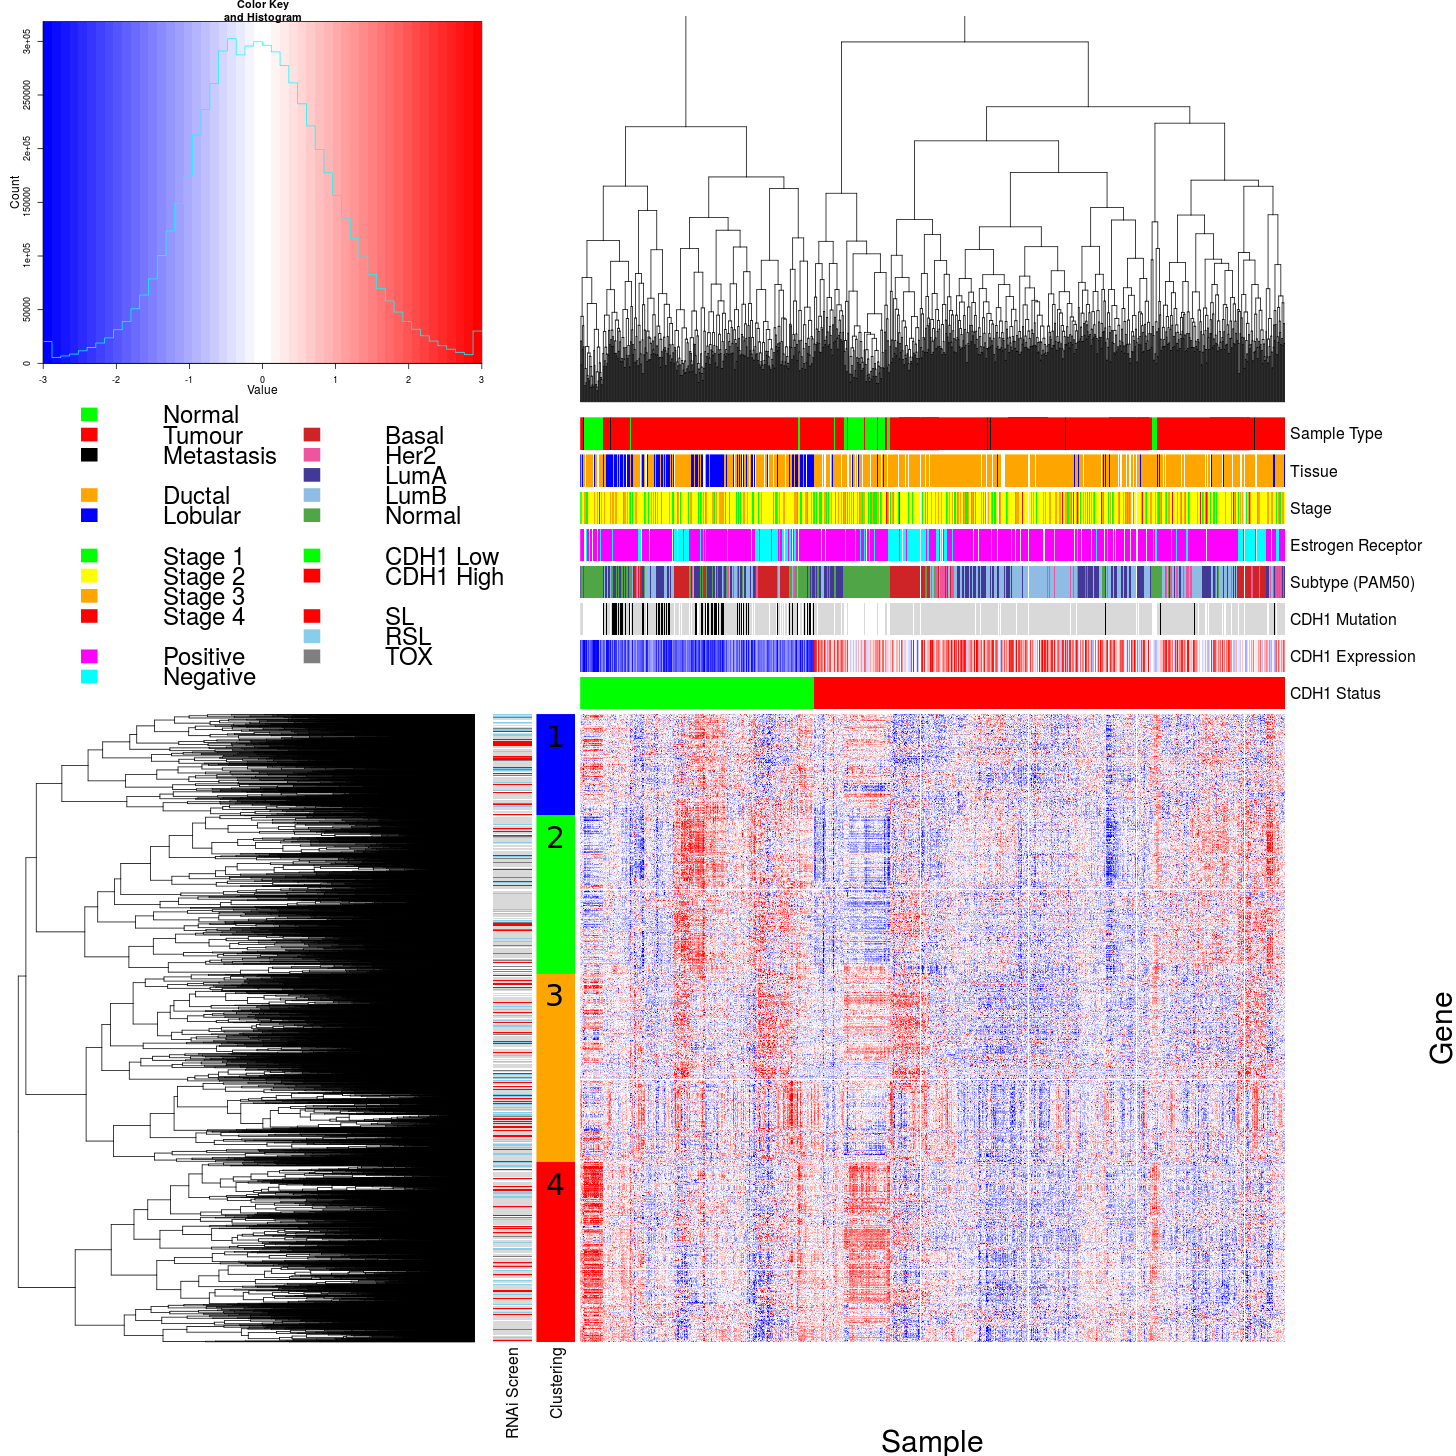
\includegraphics{CDH1_Heatmaps_Genes_Split_By_CDH1_z-trans_exprSL_cordistx_Pub.png}
   }
    \caption[Synthetic lethal expression profiles of analysed samples]{\small \textbf{Synthetic lethal expression profiles of analysed samples.} Gene expression profile heatmap (correlation distance) of all samples (separated by the $\sfrac{1}{3}$ quantile of \textit{CDH1} expression) analysed in TCGA breast cancer dataset for gene expression of 4,629 candidate partners of E-cadherin (\textit{CDH1}) from SLIPT prediction (with significant FDR adjusted $p < 0.05$). Deeply clustered, inter-correlated genes form several main groups, each containing genes that were SL candidates or toxic in an siRNA screen \cite{Telford2015}. Clusters had different sample groups highly expressing the synthetic lethal candidates in \textit{CDH1} low samples, notably 'normal-like', basal, and estrogen receptor negative samples have elevated expression in one or more distinct clusters showing complexity and variation among candidate synthetic lethal partners. \textit{CDH1} low samples also contained most of samples with \textit{CDH1} mutations.
   %This suggests that multiple targets may be needed to target \textit{CDH1} deficiency across genetic backgrounds and that combination therapy may be more effective. 
}
\label{fig:slipt_expr}
\end{mdframed}
\end{figure*}

Table 5.  Gene set enrichment results for subgroups of \textit{CDH1} SL partners shows functional variation.

Figure 3.   Heatmap of RNASeq gene expression in predicted SL partners of \textit{CDH1} showing distinct subgroups of SL partners and links between SL partner expression and clinical variables.

\subsubsection{Subgroup pathway analysis}
%%committee
Synthetic lethal gene candidates for \textit{CDH1} from SLIPT performed on RNA-Seq expression data were also used for pathway over-representation analyses (as described in section \ref{methods:enrichment}). The correlation structure in the expression of candidates synthetic lethal genes in \textit{CDH1} low tumours (lowest $\sfrac{1}{3}$\textsuperscript{rd} quantile of expression) was examined for distinct biological pathways in subgroups of genes elevated in different clusters of samples including some by clinical factors such as estrogen receptor status, intrinsic (PAM50) subtype \citep{Parker2009}, and somatic mutation (of highest impact genes) against these gene clusters.


%%paper
As shown by the most over-represented pathways in Table \ref{tab:pathway_clusters}, each correlated cluster of candidate synthetic lethal partners of \textit{CDH1} contains functionally different genes. %Each correlated subgroup of synthetic lethal candidate genes has markedly different biological functions.
Cluster 1 contains genes with less evidence of over-represented pathways than other clusters, corresponding to less correlation between genes within the cluster, and to it being a relatively small group. While there is some indication that collagen biosynthesis, microfibril elastic fibres, extracellular matrix, and metabolic pathways may be over-represent\-ed in Cluster 1, these results are mainly based on small pathways containing few synthetic lethal genes. Genes in Cluster 2 exhibited low expression in normal tissue samples compared to tumour samples (see Figure \ref{fig:slipt_expr}) and show compelling evidence of over-represent\-ation of post-transcriptional gene regulation and protein translation processes. Similarly, Cluster 3 has over-represent\-ation of immune signalling pathways (including chemokines, secondary messenger, and TCR signaling) and downstream intracellular signalling cascades such as G protein coupled receptor (GPCR) and  G$_{\alpha i}$ signalling events. While pathway over-represent\-ation was weaker among genes in Cluster 4, they contained intracellular signalling pathways and were highly expressed in normal samples (in contrast to Cluster 2). Cluster 4 also involved extracellular factors and stimuli such as extracellular matrix, platelet activation, ligand receptors, and retinoic acid signalling.

Based on these results, potential synthetic lethal partners of \textit{CDH1} include processes known to be dysregulated in cancer, such as translational, cytoskeletal, and immune processes. Intracellular signalling cascades such as the GPCRs and extracellular stimuli for these pathways were also implicated in potential synthetic lethality with \textit{CDH1}.


\begin{table*}[!Hp]
\caption{Pathway composition for clusters of \textit{CDH1} partners from SLIPT}
\label{tab:pathway_clusters}
\centering
%\begin{tiny}
%\makebox[\textwidth][c]{
\resizebox{0.666 \textwidth}{!}{
\begin{tabular}{lccc}
%\caption{Pathway composition for clusters of \textit{CDH1} partners from SLIPT}
%\label{tab:pathway_clusters}
  \large{\textbf{Pathways Over-represented in Cluster 1}} & \large{\textbf{Pathway Size}} & \large{\textbf{Cluster Genes}} & \large{\textbf{p-value (FDR)}} \\ %(833 genes)  
  \hline
  \rowcolor{Cluster_Blue!20}
  Collagen formation &  67 &  10 & $4.0 \times 10^{-11}$ \\
  \rowcolor{Cluster_Blue!15} 
  Extracellular matrix organisation & 238 &  21 & $1.8 \times 10^{-9}$ \\
  \rowcolor{Cluster_Blue!20} 
  Collagen biosynthesis and modifying enzymes &  56 &   8 & $1.8 \times 10^{-9}$ \\
  \rowcolor{Cluster_Blue!15} 
  Uptake and actions of bacterial toxins &  22 &   5 & $9.5 \times 10^{-9}$ \\
  \rowcolor{Cluster_Blue!20} 
  Elastic fibre formation &  37 &   6 & $1.9 \times 10^{-8}$ \\
  \rowcolor{Cluster_Blue!15} 
  Muscle contraction &  62 &   7 & $2.4 \times 10^{-7}$ \\
  \rowcolor{Cluster_Blue!20} 
  Fatty acid, triacylglycerol, and ketone body metabolism & 117 &  10 & $4.9 \times 10^{-7}$ \\
  \rowcolor{Cluster_Blue!15} 
  XBP1(S) activates chaperone genes &  51 &   6 & $6.6 \times 10^{-7}$ \\
  \rowcolor{Cluster_Blue!20} 
  IRE1alpha activates chaperones &  54 &   6 & $1.2 \times 10^{-6}$ \\
  \rowcolor{Cluster_Blue!15} 
  Neurotoxicity of clostridium toxins &  10 &   3 & $1.3 \times 10^{-6}$ \\
  \rowcolor{Cluster_Blue!20} 
  Retrograde neurotrophin signalling &  10 &   3 & $1.3 \times 10^{-6}$ \\
  \rowcolor{Cluster_Blue!15} 
  Assembly of collagen fibrils and other multimeric structures &  40 &   5 & $1.9 \times 10^{-6}$ \\
  \rowcolor{Cluster_Blue!20} 
  Collagen degradation &  58 &   6 & $2.0 \times 10^{-6}$ \\
  \rowcolor{Cluster_Blue!15} 
  Arachidonic acid metabolism &  41 &   5 & $2.1 \times 10^{-6}$ \\
  \rowcolor{Cluster_Blue!20} 
  Synthesis of PA &  26 &   4 & $3.0 \times 10^{-6}$ \\
  \rowcolor{Cluster_Blue!15} 
  Signaling by NOTCH &  80 &   7 & $3.3 \times 10^{-6}$ \\
  \rowcolor{Cluster_Blue!20} 
  Signalling to RAS &  27 &   4 & $3.7 \times 10^{-6}$ \\
  \rowcolor{Cluster_Blue!15} 
  Integrin cell surface interactions &  82 &   7 & $4.2 \times 10^{-6}$ \\
  \rowcolor{Cluster_Blue!20} 
  Smooth Muscle Contraction &  28 &   4 & $4.4 \times 10^{-6}$ \\
  \rowcolor{Cluster_Blue!15} 
  ECM proteoglycans &  66 &   6 & $6.3 \times 10^{-6}$ \\ 
  \hline
  \\
  \cellcolor{white} \large{\textbf{Pathways Over-represented in Cluster 2}} & \large{\textbf{Pathway Size}} & \large{\textbf{Cluster Genes}} & \large{\textbf{p-value (FDR)}} \\ %(833 genes)  
  \hline
  \rowcolor{Cluster_Green!20}
  Eukaryotic Translation Elongation &  86 &  75 & $1.1 \times 10^{-181}$ \\
  \rowcolor{Cluster_Green!15} 
  Viral mRNA Translation &  81 &  72 & $9.8 \times 10^{-179}$ \\
  \rowcolor{Cluster_Green!20} 
  Peptide chain elongation &  83 &  72 & $1.9 \times 10^{-175}$ \\
  \rowcolor{Cluster_Green!15} 
  Eukaryotic Translation Termination &  83 &  72 & $1.9 \times 10^{-175}$ \\
  \rowcolor{Cluster_Green!20} 
  Formation of a pool of free 40S subunits &  93 &  75 & $1.9 \times 10^{-171}$ \\
  \rowcolor{Cluster_Green!15} 
  Nonsense Mediated Decay independent of the Exon Junction Complex &  88 &  72 & $9.9 \times 10^{-168}$ \\
  \rowcolor{Cluster_Green!20} 
  L13a-mediated translational silencing of Ceruloplasmin expression & 103 &  75 & $3.0 \times 10^{-159}$ \\
  \rowcolor{Cluster_Green!15} 
  3' -UTR-mediated translational regulation & 103 &  75 & $3.0 \times 10^{-159}$ \\
  \rowcolor{Cluster_Green!20} 
  Nonsense-Mediated Decay & 103 &  75 & $3.0 \times 10^{-159}$ \\
  \rowcolor{Cluster_Green!15} 
  Nonsense Mediated Decay enhanced by the Exon Junction Complex & 103 &  75 & $3.0 \times 10^{-159}$ \\
  \rowcolor{Cluster_Green!20} 
  SRP-dependent cotranslational protein targeting to membrane & 104 &  75 & $3.2 \times 10^{-158}$ \\
  \rowcolor{Cluster_Green!15} 
  GTP hydrolysis and joining of the 60S ribosomal subunit & 104 &  75 & $3.2 \times 10^{-158}$ \\
  \rowcolor{Cluster_Green!20} 
  Eukaryotic Translation Initiation & 111 &  75 & $4.5 \times 10^{-151}$ \\
  \rowcolor{Cluster_Green!15} 
  Cap-dependent Translation Initiation & 111 &  75 & $4.5 \times 10^{-151}$ \\
  \rowcolor{Cluster_Green!20} 
  Influenza Infection & 117 &  75 & $1.4 \times 10^{-145}$ \\
  \rowcolor{Cluster_Green!15} 
  Influenza Viral RNA Transcription and Replication & 108 &  72 & $5.7 \times 10^{-145}$ \\
  \rowcolor{Cluster_Green!20} 
  Translation & 141 &  81 & $8.0 \times 10^{-143}$ \\
  \rowcolor{Cluster_Green!15} 
  Influenza Life Cycle & 112 &  72 & $2.3 \times 10^{-141}$ \\
  \rowcolor{Cluster_Green!20} 
  Infectious disease & 347 & 103 & $2.2 \times 10^{-95}$ \\
  \rowcolor{Cluster_Green!15} 
  Formation of the ternary complex, and subsequently, the 43S complex &  47 &  33 & $6.8 \times 10^{-80}$ \\
  \hline
  \\
  \cellcolor{white} \large{\textbf{Pathways Over-represented in Cluster 3}} & \large{\textbf{Pathway Size}} & \large{\textbf{Cluster Genes}} & \large{\textbf{p-value (FDR)}} \\ %(833 genes)  
  \hline
  \rowcolor{Cluster_Orange!30}
  Adaptive Immune System & 412 &  90 & $6.1 \times 10^{-61}$ \\
  \rowcolor{Cluster_Orange!20} 
  Chemokine receptors bind chemokines &  52 &  27 & $6.7 \times 10^{-56}$ \\
  \rowcolor{Cluster_Orange!30} 
  Generation of second messenger molecules &  29 &  21 & $6.5 \times 10^{-55}$ \\
  \rowcolor{Cluster_Orange!20} 
  Immunoregulatory interactions between a Lymphoid and a non-Lymphoid cell &  64 &  29 & $6.5 \times 10^{-55}$ \\
  \rowcolor{Cluster_Orange!30} 
  TCR signalling &  62 &  27 & $8.9 \times 10^{-51}$ \\
  \rowcolor{Cluster_Orange!20} 
  Peptide ligand-binding receptors & 161 &  40 & $1.5 \times 10^{-45}$ \\
  \rowcolor{Cluster_Orange!30} 
  Translocation of ZAP-70 to Immunological synapse &  16 &  14 & $3.1 \times 10^{-43}$ \\
  \rowcolor{Cluster_Orange!20} 
  Costimulation by the CD28 family &  51 &  22 & $4.0 \times 10^{-43}$ \\
  \rowcolor{Cluster_Orange!30} 
  PD-1 signalling &  21 &  15 & $4.0 \times 10^{-41}$ \\
  \rowcolor{Cluster_Orange!20} 
  Class A/1 (Rhodopsin-like receptors) & 258 &  50 & $6.7 \times 10^{-41}$ \\
  \rowcolor{Cluster_Orange!30} 
  Phosphorylation of CD3 and TCR zeta chains &  18 &  14 & $1.3 \times 10^{-40}$ \\
  \rowcolor{Cluster_Orange!20} 
  Interferon gamma signalling &  74 &  24 & $5.0 \times 10^{-39}$ \\
  \rowcolor{Cluster_Orange!30} 
  GPCR ligand binding & 326 &  57 & $1.8 \times 10^{-38}$ \\
  \rowcolor{Cluster_Orange!20} 
  Cytokine Signaling in Immune system & 268 &  48 & $8.9 \times 10^{-37}$ \\
  \rowcolor{Cluster_Orange!30} 
  Downstream TCR signalling &  45 &  18 & $1.8 \times 10^{-35}$ \\
  \rowcolor{Cluster_Orange!20} 
  G$_{\alpha i}$ signalling events & 167 &  33 & $2.2 \times 10^{-33}$ \\
  \rowcolor{Cluster_Orange!30} 
  Cell surface interactions at the vascular wall &  99 &  21 & $1.3 \times 10^{-26}$ \\
  \rowcolor{Cluster_Orange!20} 
  Interferon Signalling & 164 &  28 & $1.7 \times 10^{-26}$ \\
  \rowcolor{Cluster_Orange!30} 
  Extracellular matrix organisation & 238 &  35 & $2.7 \times 10^{-25}$ \\
  \rowcolor{Cluster_Orange!20} 
  Antigen activates B Cell Receptor leading to generation of second messengers &  32 &  12 & $7.2 \times 10^{-25}$ \\
   \hline
  \\ 
  \cellcolor{white} \large{\textbf{Pathways Over-represented in Cluster 4}} & \large{\textbf{Pathway Size}} & \large{\textbf{Cluster Genes}} & \large{\textbf{p-value (FDR)}} \\ %(833 genes)  
  \hline 
  \rowcolor{Cluster_Red!20}
  Extracellular matrix organisation & 238 &  48 & $8.0 \times 10^{-41}$ \\
  \rowcolor{Cluster_Red!15} 
  Class A/1 (Rhodopsin-like receptors) & 258 &  47 & $2.8 \times 10^{-36}$ \\
  \rowcolor{Cluster_Red!20} 
  GPCR ligand binding & 326 &  54 & $2.1 \times 10^{-34}$ \\
  \rowcolor{Cluster_Red!15} 
  G$_{\alpha s}$ signalling events &  83 &  22 & $1.4 \times 10^{-31}$ \\
  \rowcolor{Cluster_Red!20} 
  GPCR downstream signalling & 472 &  68 & $1.1 \times 10^{-29}$ \\
  \rowcolor{Cluster_Red!15} 
  Haemostasis & 423 &  61 & $3.3 \times 10^{-29}$ \\
  \rowcolor{Cluster_Red!20} 
  Platelet activation, signalling and aggregation & 180 &  31 & $7.1 \times 10^{-28}$ \\
  \rowcolor{Cluster_Red!15} 
  Binding and Uptake of Ligands by Scavenger Receptors &  40 &  14 & $9.9 \times 10^{-27}$ \\
  \rowcolor{Cluster_Red!20} 
  RA biosynthesis pathway &  22 &  11 & $2.5 \times 10^{-26}$ \\
  \rowcolor{Cluster_Red!15} 
  Response to elevated platelet cytosolic Ca$^{2+}$ &  82 &  19 & $3.0 \times 10^{-26}$ \\
  \rowcolor{Cluster_Red!20} 
  Developmental Biology & 420 &  57 & $3.5 \times 10^{-26}$ \\
  \rowcolor{Cluster_Red!15} 
  G$_{\alpha i}$ signalling events & 167 &  28 & $7.3 \times 10^{-26}$ \\
  \rowcolor{Cluster_Red!20} 
  Platelet degranulation &  77 &  18 & $1.6 \times 10^{-25}$ \\
  \rowcolor{Cluster_Red!15} 
  Gastrin-CREB signalling pathway via PKC and MAPK & 171 &  28 & $2.5 \times 10^{-25}$ \\
  \rowcolor{Cluster_Red!20} 
  Muscle contraction &  62 &  16 & $4.7 \times 10^{-25}$ \\
  \rowcolor{Cluster_Red!15} 
  G$_{\alpha q}$ signalling events & 150 &  25 & $3.2 \times 10^{-24}$ \\
  \rowcolor{Cluster_Red!20} 
  Retinoid metabolism and transport &  34 &  12 & $5.0 \times 10^{-24}$ \\
  \rowcolor{Cluster_Red!15} 
  Phase 1 - Functionalisation of compounds &  67 &  16 & $6.5 \times 10^{-24}$ \\
  \rowcolor{Cluster_Red!20} 
  Signalling by Retinoic Acid &  42 &  13 & $6.7 \times 10^{-24}$ \\
  \rowcolor{Cluster_Red!15} 
  Degradation of the extracellular matrix & 102 &  19 & $1.4 \times 10^{-22}$ \\ 
  \hline
\end{tabular}
}
\end{table*}




\begin{table*}[!Hp]
\caption{Pathway composition for clusters of \textit{CDH1} partners from mtSLIPT}
\label{tab:pathway_clusters_mtSL}
\centering
%\begin{tiny}
%\makebox[\textwidth][c]{
\resizebox{0.666 \textwidth}{!}{
\begin{tabular}{lccc}
%\caption{Pathway composition for clusters of \textit{CDH1} partners from SLIPT}
%\label{tab:pathway_clusters}
  \large{\textbf{Pathways Over-represented in Cluster 1}} & \large{\textbf{Pathway Size}} & \large{\textbf{Cluster Genes}} & \large{\textbf{p-value (FDR)}} \\ %(833 genes)  
  \hline
  \rowcolor{Cluster_Blue!20}
  G$_{\alpha s}$ signalling events &  83 &  19 & $5.1 \times 10^{-25}$ \\ 
  \rowcolor{Cluster_Blue!15}
  Extracellular matrix organization & 238 &  30 & $1.4 \times 10^{-18}$ \\ 
  \rowcolor{Cluster_Blue!20} 
  Hemostasis & 422 &  46 & $2.7 \times 10^{-16}$ \\ 
  \rowcolor{Cluster_Blue!15} 
  Aquaporin-mediated transport &  32 &   9 & $2.7 \times 10^{-16}$ \\ 
  \rowcolor{Cluster_Blue!20} 
  Transcriptional regulation of white adipocyte differentiation &  56 &  11 & $1.7 \times 10^{-15}$ \\ 
  \rowcolor{Cluster_Blue!15} 
  Degradation of the extracellular matrix & 102 &  15 & $1.7 \times 10^{-15}$ \\ 
  \rowcolor{Cluster_Blue!20} 
  Integration of energy metabolism &  84 &  13 & $8.8 \times 10^{-15}$ \\ 
  \rowcolor{Cluster_Blue!15} 
  GPCR downstream signaling & 472 &  48 & $2.8 \times 10^{-14}$ \\ 
  \rowcolor{Cluster_Blue!20} 
  G$_{\alpha z}$ signalling events &  15 &   6 & $5 \times 10^{-14}$ \\ 
  \rowcolor{Cluster_Blue!15} 
  Molecules associated with elastic fibres &  33 &   8 & $5.4 \times 10^{-14}$ \\ 
  \rowcolor{Cluster_Blue!20} 
  Phase 1 - Functionalization of compounds &  67 &  11 & $5.6 \times 10^{-14}$ \\ 
  \rowcolor{Cluster_Blue!15} 
  Platelet activation, signaling and aggregation & 179 &  20 & $5.6 \times 10^{-14}$ \\ 
  \rowcolor{Cluster_Blue!20} 
  Vasopressin regulates renal water homeostasis via Aquaporins &  24 &   7 & $6.1 \times 10^{-14}$ \\ 
  \rowcolor{Cluster_Blue!15} 
  Elastic fibre formation &  37 &   8 & $3 \times 10^{-13}$ \\ 
  \rowcolor{Cluster_Blue!20} 
  Calmodulin induced events &  27 &   7 & $3.3 \times 10^{-13}$ \\ 
  \rowcolor{Cluster_Blue!15} 
  CaM pathway &  27 &   7 & $3.3 \times 10^{-13}$ \\ 
  \rowcolor{Cluster_Blue!20} 
  cGMP effects &  18 &   6 & $3.6 \times 10^{-13}$ \\ 
  \rowcolor{Cluster_Blue!15} 
  G$_{\alpha i}$ signalling events & 167 &  18 & $6.3 \times 10^{-13}$ \\ 
  \rowcolor{Cluster_Blue!20} 
  Ca-dependent events &  29 &   7 & $8.2 \times 10^{-13}$ \\ 
  \rowcolor{Cluster_Blue!15} 
  Binding and Uptake of Ligands by Scavenger Receptors &  40 &   8 & $8.2 \times 10^{-13}$ \\ 
  \hline
  \\
  \cellcolor{white} \large{\textbf{Pathways Over-represented in Cluster 2}} & \large{\textbf{Pathway Size}} & \large{\textbf{Cluster Genes}} & \large{\textbf{p-value (FDR)}} \\ %(833 genes)  
  \hline
  \rowcolor{Cluster_Green!20}
  Olfactory Signaling Pathway &  57 &   8 & $7.1 \times 10^{-9}$ \\ 
  \rowcolor{Cluster_Green!15} 
  Assembly of the primary cilium & 149 &  14 & $8 \times 10^{-9}$ \\ 
  \rowcolor{Cluster_Green!20} 
  Sphingolipid metabolism &  62 &   8 & $9.6 \times 10^{-9}$ \\ 
  \rowcolor{Cluster_Green!15} 
  Signaling by ERBB4 & 133 &  12 & $5.1 \times 10^{-8}$ \\ 
  \rowcolor{Cluster_Green!20} 
  PI3K Cascade &  65 &   7 & $4.9 \times 10^{-7}$ \\ 
  \rowcolor{Cluster_Green!15} 
  Circadian Clock &  33 &   5 & $4.9 \times 10^{-7}$ \\ 
  \rowcolor{Cluster_Green!20} 
  Nuclear signaling by ERBB4 &  34 &   5 & $4.9 \times 10^{-7}$ \\ 
  \rowcolor{Cluster_Green!15} 
  Intraflagellar transport &  35 &   5 & $4.9 \times 10^{-7}$ \\ 
  \rowcolor{Cluster_Green!20} 
  PI3K events in ERBB4 signaling &  87 &   8 & $4.9 \times 10^{-7}$ \\ 
  \rowcolor{Cluster_Green!15} 
  PIP3 activates AKT signaling &  87 &   8 & $4.9 \times 10^{-7}$ \\ 
  \rowcolor{Cluster_Green!20} 
  PI3K events in ERBB2 signaling &  87 &   8 & $4.9 \times 10^{-7}$ \\ 
  \rowcolor{Cluster_Green!15} 
  PI-3K cascade:FGFR1 &  87 &   8 & $4.9 \times 10^{-7}$ \\ 
  \rowcolor{Cluster_Green!20} 
  PI-3K cascade:FGFR2 &  87 &   8 & $4.9 \times 10^{-7}$ \\ 
  \rowcolor{Cluster_Green!15} 
  PI-3K cascade:FGFR3 &  87 &   8 & $4.9 \times 10^{-7}$ \\ 
  \rowcolor{Cluster_Green!20} 
  PI-3K cascade:FGFR4 &  87 &   8 & $4.9 \times 10^{-7}$ \\ 
  \rowcolor{Cluster_Green!15} 
  Deadenylation of mRNA &  22 &   4 & $5.6 \times 10^{-7}$ \\ 
  \rowcolor{Cluster_Green!20} 
  PI3K/AKT activation &  90 &   8 & $5.6 \times 10^{-7}$ \\ 
  \rowcolor{Cluster_Green!15} 
  Cargo trafficking to the periciliary membrane &  38 &   5 & $5.6 \times 10^{-7}$ \\ 
  \rowcolor{Cluster_Green!20} 
  Signaling by Hedgehog & 108 &   9 & $5.6 \times 10^{-7}$ \\ 
  \rowcolor{Cluster_Green!15} 
  Downstream signal transduction & 143 &  11 & $5.6 \times 10^{-7}$ \\ 
  \hline
  \\
  \cellcolor{white} \large{\textbf{Pathways Over-represented in Cluster 3}} & \large{\textbf{Pathway Size}} & \large{\textbf{Cluster Genes}} & \large{\textbf{p-value (FDR)}} \\ %(833 genes)  
  \hline
  \rowcolor{Cluster_Orange!30}
  Eukaryotic Translation Elongation &  86 &  55 & $1.1 \times 10^{-112}$ \\ 
  \rowcolor{Cluster_Orange!20} 
  Peptide chain elongation &  83 &  54 & $1.3 \times 10^{-112}$ \\ 
  \rowcolor{Cluster_Orange!30} 
  Viral mRNA Translation &  81 &  53 & $1.6 \times 10^{-111}$ \\ 
  \rowcolor{Cluster_Orange!20} 
  Eukaryotic Translation Termination &  83 &  53 & $7.1 \times 10^{-110}$ \\ 
  \rowcolor{Cluster_Orange!30} 
  Nonsense Mediated Decay independent of the Exon Junction Complex &  88 &  54 & $1 \times 10^{-108}$ \\ 
  \rowcolor{Cluster_Orange!20} 
  Formation of a pool of free 40S subunits &  93 &  53 & $4.1 \times 10^{-102}$ \\ 
  \rowcolor{Cluster_Orange!30} 
  Nonsense-Mediated Decay & 103 &  54 & $3.9 \times 10^{-98}$ \\ 
  \rowcolor{Cluster_Orange!20} 
  Nonsense Mediated Decay enhanced by the Exon Junction Complex & 103 &  54 & $3.9 \times 10^{-98}$ \\ 
  \rowcolor{Cluster_Orange!30} 
  L13a-mediated translational silencing of Ceruloplasmin expression & 103 &  53 & $1.2 \times 10^{-95}$ \\ 
  \rowcolor{Cluster_Orange!20} 
  3' -UTR-mediated translational regulation & 103 &  53 & $1.2 \times 10^{-95}$ \\ 
  \rowcolor{Cluster_Orange!30} 
  SRP-dependent cotranslational protein targeting to membrane & 104 &  53 & $4.3 \times 10^{-95}$ \\ 
  \rowcolor{Cluster_Orange!20} 
  GTP hydrolysis and joining of the 60S ribosomal subunit & 104 &  53 & $4.3 \times 10^{-95}$ \\ 
  \rowcolor{Cluster_Orange!30} 
  Influenza Viral RNA Transcription and Replication & 108 &  53 & $9.6 \times 10^{-93}$ \\ 
  \rowcolor{Cluster_Orange!20} 
  Eukaryotic Translation Initiation & 111 &  53 & $4.2 \times 10^{-91}$ \\ 
  \rowcolor{Cluster_Orange!30} 
  Cap-dependent Translation Initiation & 111 &  53 & $4.2 \times 10^{-91}$ \\ 
  \rowcolor{Cluster_Orange!20} 
  Influenza Life Cycle & 112 &  53 & $1.4 \times 10^{-90}$ \\ 
  \rowcolor{Cluster_Orange!30} 
  Influenza Infection & 117 &  53 & $6.2 \times 10^{-88}$ \\ 
  \rowcolor{Cluster_Orange!20} 
  Translation & 141 &  55 & $3 \times 10^{-81}$ \\ 
  \rowcolor{Cluster_Orange!30} 
  Formation of the ternary complex, and subsequently, the 43S complex &  47 &  23 & $2.3 \times 10^{-48}$ \\ 
  \rowcolor{Cluster_Orange!20} 
  Translation initiation complex formation &  54 &  23 & $9.1 \times 10^{-45}$ \\ 
  \hline
  \\ 
  \cellcolor{white} \large{\textbf{Pathways Over-represented in Cluster 4}} & \large{\textbf{Pathway Size}} & \large{\textbf{Cluster Genes}} & \large{\textbf{p-value (FDR)}} \\ %(833 genes)  
  \hline 
  \rowcolor{Cluster_Red!20}
  ECM proteoglycans &  66 &  10 & $2.9 \times 10^{-11}$ \\ 
  \rowcolor{Cluster_Red!15} 
  deactivation of the beta-catenin transactivating complex &  38 &   7 & $5.1 \times 10^{-10}$ \\ 
  \rowcolor{Cluster_Red!20} 
  Arachidonic acid metabolism &  41 &   7 & $1.1 \times 10^{-9}$ \\ 
  \rowcolor{Cluster_Red!15} 
  G_${\alpha q}$ signalling events & 149 &  14 & $4 \times 10^{-9}$ \\ 
  \rowcolor{Cluster_Red!20} 
  HS-GAG degradation &  21 &   5 & $4.5 \times 10^{-9}$ \\ 
  \rowcolor{Cluster_Red!15} 
  Uptake and actions of bacterial toxins &  22 &   5 & $6.1 \times 10^{-9}$ \\ 
  \rowcolor{Cluster_Red!20} 
  Gastrin-CREB signalling pathway via PKC and MAPK & 170 &  15 & $6.1 \times 10^{-9}$ \\ 
  \rowcolor{Cluster_Red!15} 
  RNA Polymerase I, RNA Polymerase III, and Mitochondrial Transcription \textcolor{Cluster_Red!15}{ll}  &  64 &   8 & $6.1 \times 10^{-9}$ \\ 
  \rowcolor{Cluster_Red!20} 
  Non-integrin membrane-ECM interactions &  53 &   7 & $1.5 \times 10^{-8}$ \\ 
  \rowcolor{Cluster_Red!15} 
  Syndecan interactions &  25 &   5 & $1.5 \times 10^{-8}$ \\ 
  \rowcolor{Cluster_Red!20} 
  NOTCH1 Intracellular Domain Regulates Transcription &  40 &   6 & $2.3 \times 10^{-8}$ \\ 
  \rowcolor{Cluster_Red!15} 
  Synthesis of Leukotrienes and Eoxins &  15 &   4 & $3.2 \times 10^{-8}$ \\ 
  \rowcolor{Cluster_Red!20} 
  Signaling by NOTCH1 &  59 &   7 & $5.3 \times 10^{-8}$ \\ 
  \rowcolor{Cluster_Red!15} 
  Regulation of insulin secretion &  44 &   6 & $6 \times 10^{-8}$ \\ 
  \rowcolor{Cluster_Red!20} 
  Metabolism of lipids and lipoproteins & 471 &  37 & $8.2 \times 10^{-8}$ \\ 
  \rowcolor{Cluster_Red!15} 
  Signaling by NOTCH &  80 &   8 & $1.2 \times 10^{-7}$ \\ 
  \rowcolor{Cluster_Red!20} 
  Platelet activation, signaling and aggregation & 179 &  14 & $1.2 \times 10^{-7}$ \\ 
  \rowcolor{Cluster_Red!15} 
  Recruitment of mitotic centrosome proteins and complexes &  64 &   7 & $1.2 \times 10^{-7}$ \\ 
  \rowcolor{Cluster_Red!20} 
  Centrosome maturation &  64 &   7 & $1.2 \times 10^{-7}$ \\ 
  \rowcolor{Cluster_Red!15} 
  Biological oxidations & 133 &  11 & $1.5 \times 10^{-7}$ \\ 
  \hline
\end{tabular}
}
\end{table*}




\section{Comparison of synthetic lethal gene candidates}

\subsection{Comparison with differential expression}

\subsection{Comparison with correlation}

\subsection{Comparison with primary siRNA screen candidates}

Gene candidates were compared between computational and experimental screening approaches in Figure \ref{fig:Venn_allgenes}. The number of genes detected by both methods did not produce a significant overlap but these may be difficult to compare due to vast differences between the detection methods. These intersecting genes could be useful in drug triage as they were replicated across both methods and pathway over-represent\-ation differed between the sections of the Venn diagram (see Figure \ref{fig:Venn_allgenes}).

\begin{figure}[!ht]
\begin{mdframed}
  \centering
  \resizebox{0.66 \columnwidth}{!}{
    \includegraphics{Venn_exprSL_siRNA_allgenes_reduced_Pub.png}
   }
    \caption[Comparison of SLIPT to siRNA]{\small \textbf{Comparison of SLIPT to siRNA.} Testing the overlap of gene candidates for E-cadherin synthetic lethal partners between computational (SLIPT) and experimental screening (siRNA) approaches. The $\chi^2$ test suggests that the overlap is no more than would be expected by chance ($p = 0.281$). %A Venn diagram of all 16298 genes tested by both approaches.
}
\label{fig:Venn_allgenes}
\end{mdframed}
\end{figure}

\begin{figure}[!ht]
\begin{mdframed}
  \centering
  \resizebox{0.66 \columnwidth}{!}{
    \includegraphics{Venn_mtSL_siRNA_allgenes_reduced_Pub.png}
   }
    \caption[Comparison of mtSLIPT to siRNA]{\small \textbf{Comparison of mtSLIPT to siRNA.} Testing the overlap of gene candidates for E-cadherin synthetic lethal partners between computational (SLIPT) and experimental screening (siRNA) approaches. The $\chi^2$ test suggests that the overlap is no more than would be expected by chance ($p = 0.281$). %A Venn diagram of all 16298 genes tested by both approaches.
}
\label{fig:Venn_allgenes_mtSL}
\end{mdframed}
\end{figure}

The overlap between synthetic lethal from bioinformatics SLIPT predictions and siRNA screening has raised other questions including whether the number of genes and pathways enriched would be expected by chance. This of particular concern since the siRNA candidate genes themselves are highly enriched for particular pathways so selecting any intersect with them would be enriched for these pathways. The siRNA data is also based on cell line models which have limitations in application to a genetically variable patient population with a complex tumour microenvironment interacting with immune cells. One approach is to compare the candidate genes is to exclude genes that were not tested in both systems, such as those not expressed in cell lines or those with more than $\sfrac{1}{3}$ of TCGA patients without any RNA Seq reads so the lowest quantile cannot be defined for SLIPT analysis. Another approach is to test whether pathways are enriched in randomly sampled genes, comparing many “resampled” or “permutations” of these genes to the enrichment statistics observed for these pathways in the SLIPT candidates and their intersection with the siRNA hits shows whether we detect these pathways more than we expect by chance.

Both of these are being applied with developing a method and overcoming technical challenges for the latter being the focus of recent work. The main challenge at the moment is to compare SLIPT results to experimental candidates and explain why so few genes (and so many pathways) overlap.

As discussed above, comparing genes between experimental screen candidates and prediction from TCGA expression data has been difficult. Figure 3 summarises the approaches to comparing genes accounting for some of the differences between the datasets. Of particular concern are the over-represented pathways in genes detected by both methods. There is no statistical evidence that SLIPT predicted genes or siRNA candidates are enriched in with each other. The siRNA candidates themselves are over-represented with many pathways including GPCRs so any intersection with these would contain some of these pathways. Whether these pathways are contained in the intersection more than expected by chance is the problem the two approaches below were designed to tackle.

\subsubsection{Comparison of screen at pathway level}

These pathway analyses correspond to genes separated into SLIPT or siRNA screen candidates unique to either method or detected by both (Table \ref{tab:Venn_over-representation}). The SLIPT-specific gene candidates were involved most strongly with translational and immune regulatory pathways, which were also identified in the clustering analysis (Table \ref{tab:pathway_clusters}). The genes detected only by the siRNA screen had over-represent\-ation of cell signalling pathways, including many containing genes known to be involved in cancer (e.g., MAPK, PDGF, ERBB2, and FGFR), with the detection of Class A GPCRs supporting the independent analyses by  Telford \textit{et al.} \cite{Telford2015}.

The intersection of computational and experimental synthetic lethal partners of \textit{CDH1} has stronger evidence for over-represent\-ation of GPCR pathways and more specific subclasses, such as visual phototransduction ($p=6.9 \times 10^{-10}$) and G$_{\alpha s}$ signalling events ($p=1.7 \times 10^{-7}$), than other signalling pathways

\begin{table*}[!Hp]
\caption{Pathway composition for \textit{CDH1} partners from SLIPT and siRNA screening}
\label{tab:Venn_over-representation}
\centering
\resizebox{0.8 \textwidth}{!}{
\begin{tabular}{sl^c^c^c}
\rowstyle{\bfseries}
  Predicted only by SLIPT (4025 genes) & Pathway Size & Genes Identified & p-value (FDR) \\ 
  \hline
  \rowcolor{Cluster_Red!20}
  Eukaryotic Translation Elongation &  80 &  75 & $1.5 \times 10^{-182}$ \\
  \rowcolor{Cluster_Red!15} 
  Peptide chain elongation &  77 &  72 & $2.9 \times 10^{-176}$ \\
  \rowcolor{Cluster_Red!20} 
  Viral mRNA Translation &  75 &  70 & $4.9 \times 10^{-172}$ \\
  \rowcolor{Cluster_Red!15} 
  Eukaryotic Translation Termination &  76 &  70 & $5.9 \times 10^{-170}$ \\
  \rowcolor{Cluster_Red!20} 
  Formation of a pool of free 40S subunits &  87 &  74 & $9.5 \times 10^{-166}$ \\
  \rowcolor{Cluster_Red!15} 
  Nonsense Mediated Decay independent of the Exon Junction Complex &  81 &  70 & $1.2 \times 10^{-160}$ \\
  \rowcolor{Cluster_Red!20} 
  L13a-mediated translational silencing of Ceruloplasmin expression &  97 &  75 & $3.8 \times 10^{-155}$ \\
  \rowcolor{Cluster_Red!15} 
  3' -UTR-mediated translational regulation &  97 &  75 & $3.8 \times 10^{-155}$ \\
  \rowcolor{Cluster_Red!20} 
  GTP hydrolysis and joining of the 60S ribosomal subunit &  98 &  75 & $6.0 \times 10^{-154}$ \\
  \rowcolor{Cluster_Red!15} 
  Nonsense-Mediated Decay &  96 &  73 & $5.2 \times 10^{-150}$ \\
  \rowcolor{Cluster_Red!20} 
  Nonsense Mediated Decay enhanced by the Exon Junction Complex &  96 &  73 & $5.2 \times 10^{-150}$ \\
  \rowcolor{Cluster_Red!15} 
  SRP-dependent cotranslational protein targeting to membrane &  97 &  73 & $7.8 \times 10^{-149}$ \\
  \rowcolor{Cluster_Red!20} 
  Eukaryotic Translation Initiation & 105 &  75 & $4.7 \times 10^{-146}$ \\
  \rowcolor{Cluster_Red!15} 
  Cap-dependent Translation Initiation & 105 &  75 & $4.7 \times 10^{-146}$ \\
  \rowcolor{Cluster_Red!20} 
  Translation & 133 &  83 & $4.0 \times 10^{-142}$ \\
  \rowcolor{Cluster_Red!15} 
  Influenza Viral RNA Transcription and Replication & 102 &  71 & $2.9 \times 10^{-137}$ \\
  \rowcolor{Cluster_Red!20} 
  Influenza Infection & 111 &  74 & $3.7 \times 10^{-137}$ \\
  \rowcolor{Cluster_Red!15} 
  Influenza Life Cycle & 106 &  71 & $2.3 \times 10^{-133}$ \\
  \rowcolor{Cluster_Red!20} 
  Infectious disease & 326 & 125 & $4.2 \times 10^{-120}$ \\
  \rowcolor{Cluster_Red!15} 
  Extracellular matrix organisation & 189 &  77 & $5.4 \times 10^{-95}$ \\
  \hline
  \\
  \rowstyle{\bfseries}
  Detected only by siRNA screen (1599 genes) & Pathway Size & Genes Identified & p-value (FDR) \\ 
  \hline
  \rowcolor{Cluster_Blue!20}
  Class A/1 (Rhodopsin-like receptors) & 282 &  44 & $1.3 \times 10^{-27}$ \\
  \rowcolor{Cluster_Blue!15} 
  GPCR ligand binding & 363 &  52 & $5.8 \times 10^{-26}$ \\
  \rowcolor{Cluster_Blue!20} 
  G$_{\alpha q}$ signalling events & 159 &  26 & $6.7 \times 10^{-23}$ \\
  \rowcolor{Cluster_Blue!15} 
  Gastrin-CREB signalling pathway via PKC and MAPK & 180 &  27 & $2.0 \times 10^{-21}$ \\
  \rowcolor{Cluster_Blue!20} 
  G$_{\alpha i}$ signalling events & 184 &  27 & $5.3 \times 10^{-21}$ \\
  \rowcolor{Cluster_Blue!15} 
  Downstream signal transduction & 146 &  23 & $7.6 \times 10^{-21}$ \\
  \rowcolor{Cluster_Blue!20} 
  Signalling by PDGF & 172 &  25 & $4.0 \times 10^{-20}$ \\
  \rowcolor{Cluster_Blue!15} 
  Peptide ligand-binding receptors & 175 &  25 & $8.5 \times 10^{-20}$ \\
  \rowcolor{Cluster_Blue!20} 
  Signalling by ERBB2 & 146 &  22 & $1.3 \times 10^{-19}$ \\
  \rowcolor{Cluster_Blue!15} 
  DAP12 interactions & 159 &  23 & $2.6 \times 10^{-19}$ \\
  \rowcolor{Cluster_Blue!20} 
  DAP12 signalling & 149 &  22 & $2.7 \times 10^{-19}$ \\
  \rowcolor{Cluster_Blue!15} 
  Organelle biogenesis and maintenance & 264 &  33 & $5.5 \times 10^{-19}$ \\
  \rowcolor{Cluster_Blue!20} 
  Signalling by NGF & 266 &  33 & $8.2 \times 10^{-19}$ \\
  \rowcolor{Cluster_Blue!15} 
  Downstream signalling of activated FGFR1 & 134 &  20 & $1.1 \times 10^{-18}$ \\
  \rowcolor{Cluster_Blue!20} 
  Downstream signalling of activated FGFR2 & 134 &  20 & $1.1 \times 10^{-18}$ \\
  \rowcolor{Cluster_Blue!15} 
  Downstream signalling of activated FGFR3 & 134 &  20 & $1.1 \times 10^{-18}$ \\
  \rowcolor{Cluster_Blue!20} 
  Downstream signalling of activated FGFR4 & 134 &  20 & $1.1 \times 10^{-18}$ \\
  \rowcolor{Cluster_Blue!15} 
  Signalling by FGFR & 146 &  21 & $1.3 \times 10^{-18}$ \\
  \rowcolor{Cluster_Blue!20} 
  Signalling by FGFR1 & 146 &  21 & $1.3 \times 10^{-18}$ \\
  \rowcolor{Cluster_Blue!15} 
  Signalling by FGFR2 & 146 &  21 & $1.3 \times 10^{-18}$ \\
  \hline
  \\
  \rowstyle{\bfseries}
  Intersection of SLIPT and siRNA screen (604 genes) & Pathway Size & Genes Identified & p-value (FDR) \\ 
  \hline
  \rowcolor{Cluster_Red!20!Cluster_Blue!20}
  Visual phototransduction &  54 &   9 & $6.9 \times 10^{-10}$ \\
  \rowcolor{Cluster_Red!15!Cluster_Blue!15} 
  G$_{\alpha s}$ signalling events &  48 &   7 & $1.6 \times 10^{-7}$ \\
  \rowcolor{Cluster_Red!20!Cluster_Blue!20} 
  Retinoid metabolism and transport &  24 &   5 & $1.7 \times 10^{-7}$ \\
  \rowcolor{Cluster_Red!15!Cluster_Blue!15} 
  Acyl chain remodelling of PS &  10 &   3 & $6.5 \times 10^{-6}$ \\
  \rowcolor{Cluster_Red!20!Cluster_Blue!20} 
  Transcriptional regulation of white adipocyte differentiation &  51 &   6 & $6.5 \times 10^{-6}$ \\
  \rowcolor{Cluster_Red!15!Cluster_Blue!15} 
  Chemokine receptors bind chemokines &  22 &   4 & $6.5 \times 10^{-6}$ \\
  \rowcolor{Cluster_Red!20!Cluster_Blue!20} 
  Signalling by NOTCH4 &  11 &   3 & $6.9 \times 10^{-6}$ \\
  \rowcolor{Cluster_Red!15!Cluster_Blue!15} 
  Defective EXT2 causes exostoses 2 &  11 &   3 & $6.9 \times 10^{-6}$ \\
  \rowcolor{Cluster_Red!20!Cluster_Blue!20} 
  Defective EXT1 causes exostoses 1, TRPS2 and CHDS &  11 &   3 & $6.9 \times 10^{-6}$ \\
  \rowcolor{Cluster_Red!15!Cluster_Blue!15} 
  Platelet activation, signalling and aggregation & 146 &  12 & $6.9 \times 10^{-6}$ \\
  \rowcolor{Cluster_Red!20!Cluster_Blue!20} 
  Phase 1 - Functionalisation of compounds &  41 &   5 & $1.3 \times 10^{-5}$ \\
  \rowcolor{Cluster_Red!15!Cluster_Blue!15} 
  Amine ligand-binding receptors &  13 &   3 & $1.7 \times 10^{-5}$ \\
  \rowcolor{Cluster_Red!20!Cluster_Blue!20} 
  Acyl chain remodelling of PE &  14 &   3 & $2.4 \times 10^{-5}$ \\
  \rowcolor{Cluster_Red!15!Cluster_Blue!15} 
  Signalling by GPCR & 300 &  23 & $2.4 \times 10^{-5}$ \\
  \rowcolor{Cluster_Red!20!Cluster_Blue!20} 
  Molecules associated with elastic fibres &  29 &   4 & $2.6 \times 10^{-5}$ \\
  \rowcolor{Cluster_Red!15!Cluster_Blue!15} 
  DAP12 interactions & 128 &  10 & $2.6 \times 10^{-5}$ \\
  \rowcolor{Cluster_Red!20!Cluster_Blue!20} 
  Cytochrome P$_{450}$ - arranged by substrate type &  30 &   4 & $3.2 \times 10^{-5}$ \\
  \rowcolor{Cluster_Red!15!Cluster_Blue!15} 
  GPCR ligand binding & 147 &  11 & $3.8 \times 10^{-5}$ \\
  \rowcolor{Cluster_Red!20!Cluster_Blue!20} 
  Acyl chain remodelling of PC &  16 &   3 & $4.0 \times 10^{-5}$ \\
  \rowcolor{Cluster_Red!15!Cluster_Blue!15} 
  Response to elevated platelet cytosolic Ca$^{2+}$ &  66 &   6 & $4.2 \times 10^{-5}$ \\ 
  \hline
\end{tabular}
}
\end{table*}

\begin{table*}[!Hp]
\caption{Pathway composition for \textit{CDH1} partners from mtSLIPT and siRNA}
\label{tab:Venn_over-representation_mtSL}
\centering
\resizebox{0.8 \textwidth}{!}{
\begin{tabular}{sl^c^c^c}
\rowstyle{\bfseries}
  Predicted only by SLIPT (2901 genes) & Pathway Size & Genes Identified & p-value (FDR) \\ 
  \hline
  \rowcolor{Cluster_Red!20}
  Eukaryotic Translation Elongation &  87 &  57 & $2.8 \times 10^{-120}$ \\ 
  \rowcolor{Cluster_Red!15}
  Peptide chain elongation &  84 &  56 & $3.1 \times 10^{-120}$ \\ 
  \rowcolor{Cluster_Red!20}
  Eukaryotic Translation Termination &  84 &  55 & $2.8 \times 10^{-117}$ \\ 
  \rowcolor{Cluster_Red!15}
  Viral mRNA Translation &  82 &  54 & $4.1 \times 10^{-116}$ \\ 
  \rowcolor{Cluster_Red!20}
  Nonsense Mediated Decay independent of the Exon Junction Complex &  89 &  55 & $3.7 \times 10^{-113}$ \\ 
  \rowcolor{Cluster_Red!15}
  Formation of a pool of free 40S subunits &  94 &  55 & $2.8 \times 10^{-109}$ \\ 
  \rowcolor{Cluster_Red!20}
  Nonsense-Mediated Decay & 104 &  57 & $8.4 \times 10^{-108}$ \\ 
  \rowcolor{Cluster_Red!15}
  Nonsense Mediated Decay enhanced by the Exon Junction Complex & 104 &  57 & $8.4 \times 10^{-108}$ \\ 
  \rowcolor{Cluster_Red!20}
  L13a-mediated translational silencing of Ceruloplasmin expression & 104 &  56 & $3.4 \times 10^{-105}$ \\ 
  \rowcolor{Cluster_Red!15}
  3' -UTR-mediated translational regulation & 104 &  56 & $3.4 \times 10^{-105}$ \\ 
  \rowcolor{Cluster_Red!20}
  GTP hydrolysis and joining of the 60S ribosomal subunit & 105 &  56 & $1.4 \times 10^{-104}$ \\ 
  \rowcolor{Cluster_Red!15}
  Eukaryotic Translation Initiation & 112 &  56 & $2.8 \times 10^{-100}$ \\ 
  \rowcolor{Cluster_Red!20}
  Cap-dependent Translation Initiation & 112 &  56 & $2.8 \times 10^{-100}$ \\ 
  \rowcolor{Cluster_Red!15}
  SRP-dependent cotranslational protein targeting to membrane & 105 &  54 & $2.2 \times 10^{-99}$ \\ 
  \rowcolor{Cluster_Red!20}
  Influenza Viral RNA Transcription and Replication & 109 &  54 & $5.3 \times 10^{-97}$ \\ 
  \rowcolor{Cluster_Red!15}
  Influenza Life Cycle & 113 &  54 & $9.6 \times 10^{-95}$ \\ 
  \rowcolor{Cluster_Red!20}
  Influenza Infection & 118 &  55 & $1.7 \times 10^{-94}$ \\ 
  \rowcolor{Cluster_Red!15}
  Translation & 142 &  60 & $3.5 \times 10^{-94}$ \\ 
  \rowcolor{Cluster_Red!20}
  Infectious disease & 349 &  77 & $5.9 \times 10^{-62}$ \\ 
  \rowcolor{Cluster_Red!15}
  Extracellular matrix organization & 241 &  54 & $3.0 \times 10^{-52}$ \\
  \hline
  \\
  \rowstyle{\bfseries}
  Detected only by siRNA screen (1752 genes) & Pathway Size & Genes Identified & p-value (FDR) \\ 
  \hline
  \rowcolor{Cluster_Blue!20}
  Class A/1 (Rhodopsin-like receptors) & 282 &  69 & $1.9 \times 10^{-59}$ \\ 
  \rowcolor{Cluster_Blue!15}
  GPCR ligand binding & 363 &  78 & $2.7 \times 10^{-54}$ \\ 
  \rowcolor{Cluster_Blue!20}
  Peptide ligand-binding receptors & 175 &  41 & $1.5 \times 10^{-42}$ \\ 
  \rowcolor{Cluster_Blue!15}
  $G_{\alpha i}$ signalling events & 184 &  41 & $1.1 \times 10^{-40}$ \\ 
  \rowcolor{Cluster_Blue!20}
  Gastrin-CREB signalling pathway via PKC and MAPK & 180 &  37 & $1.5 \times 10^{-35}$ \\ 
  \rowcolor{Cluster_Blue!15}
  $G_{\alpha q}$ signalling events & 159 &  34 & $3.7 \times 10^{-35}$ \\ 
  \rowcolor{Cluster_Blue!20}
  DAP12 interactions & 159 &  27 & $1.1 \times 10^{-24}$ \\ 
  \rowcolor{Cluster_Blue!15}
  VEGFA-VEGFR2 Pathway &  91 &  19 & $1.0 \times 10^{-23}$ \\ 
  \rowcolor{Cluster_Blue!20}
  Downstream signal transduction & 146 &  24 & $1.9 \times 10^{-22}$ \\ 
  \rowcolor{Cluster_Blue!15}
  Signaling by VEGF &  99 &  19 & $2.6 \times 10^{-22}$ \\ 
  \rowcolor{Cluster_Blue!20}
  DAP12 signaling & 149 &  24 & $4.2 \times 10^{-22}$ \\ 
  \rowcolor{Cluster_Blue!15}
  Organelle biogenesis and maintenance & 264 &  34 & $4.3 \times 10^{-20}$ \\ 
  \rowcolor{Cluster_Blue!20}
  Downstream signaling of activated FGFR1 & 134 &  21 & $4.3 \times 10^{-20}$ \\ 
  \rowcolor{Cluster_Blue!15}
  Downstream signaling of activated FGFR2 & 134 &  21 & $4.3 \times 10^{-20}$ \\ 
  \rowcolor{Cluster_Blue!20}
  Downstream signaling of activated FGFR3 & 134 &  21 & $4.3 \times 10^{-20}$ \\ 
  \rowcolor{Cluster_Blue!15}
  Downstream signaling of activated FGFR4 & 134 &  21 & $4.3 \times 10^{-20}$ \\ 
  \rowcolor{Cluster_Blue!20}
  Signaling by ERBB2 & 146 &  22 & $5.3 \times 10^{-20}$ \\ 
  \rowcolor{Cluster_Blue!15}
  Signaling by FGFR & 146 &  22 & $5.3 \times 10^{-20}$ \\ 
  \rowcolor{Cluster_Blue!20}
  Signaling by FGFR1 & 146 &  22 & $5.3 \times 10^{-20}$ \\ 
  \rowcolor{Cluster_Blue!15}
  Signaling by FGFR2 & 146 &  22 & $5.3 \times 10^{-20}$ \\ 
  \hline
  \\
  \rowstyle{\bfseries}
  Intersection of SLIPT and siRNA screen (450 genes) & Pathway Size & Genes Identified & p-value (FDR) \\ 
  \hline
  \rowcolor{Cluster_Red!20!Cluster_Blue!20}
  HS-GAG degradation &  21 &   4 & $4.9 \times 10^{-6}$ \\ 
  \rowcolor{Cluster_Red!15!Cluster_Blue!15}
  Retinoid metabolism and transport &  39 &   5 & $4.9 \times 10^{-6}$ \\ 
  \rowcolor{Cluster_Red!20!Cluster_Blue!20}
  Platelet activation, signaling and aggregation & 186 &  13 & $4.9 \times 10^{-6}$ \\ 
  \rowcolor{Cluster_Red!15!Cluster_Blue!15}
  Signaling by NOTCH4 &  11 &   3 & $4.9 \times 10^{-6}$ \\ 
  \rowcolor{Cluster_Red!20!Cluster_Blue!20}
  $G_{\alpha s}$ signalling events & 100 &   8 & $5.0 \times 10^{-6}$ \\ 
  \rowcolor{Cluster_Red!15!Cluster_Blue!15}
  Defective EXT2 causes exostoses 2 &  12 &   3 & $5.0 \times 10^{-6}$ \\ 
  \rowcolor{Cluster_Red!20!Cluster_Blue!20}
  Defective EXT1 causes exostoses 1, TRPS2 and CHDS &  12 &   3 & $5.0 \times 10^{-6}$ \\ 
  \rowcolor{Cluster_Red!15!Cluster_Blue!15}
  Class A/1 (Rhodopsin-like receptors) & 289 &  18 & $2.2 \times 10^{-5}$ \\ 
  \rowcolor{Cluster_Red!20!Cluster_Blue!20}
  Signaling by PDGF & 173 &  11 & $2.9 \times 10^{-5}$ \\ 
  \rowcolor{Cluster_Red!15!Cluster_Blue!15}
  Circadian Clock &  34 &   4 & $2.9 \times 10^{-5}$ \\ 
  \rowcolor{Cluster_Red!20!Cluster_Blue!20}
  Signaling by ERBB4 & 139 &   9 & $4.3 \times 10^{-5}$ \\ 
  \rowcolor{Cluster_Red!15!Cluster_Blue!15}
  Role of LAT2/NTAL/LAB on calcium mobilization &  99 &   7 & $4.4 \times 10^{-5}$ \\ 
  \rowcolor{Cluster_Red!20!Cluster_Blue!20}
  Peptide ligand-binding receptors & 181 &  11 & $4.5 \times 10^{-5}$ \\ 
  \rowcolor{Cluster_Red!15!Cluster_Blue!15}
  Defective B4GALT7 causes EDS, progeroid type &  19 &   3 & $4.5 \times 10^{-5}$ \\ 
  \rowcolor{Cluster_Red!20!Cluster_Blue!20}
  Defective B3GAT3 causes JDSSDHD &  19 &   3 & $4.5 \times 10^{-5}$ \\ 
  \rowcolor{Cluster_Red!15!Cluster_Blue!15}
  Signaling by NOTCH &  80 &   6 & $4.5 \times 10^{-5}$ \\ 
  \rowcolor{Cluster_Red!20!Cluster_Blue!20}
  $G_{\alpha q}$ signalling events & 164 &  10 & $5.1 \times 10^{-5}$ \\ 
  \rowcolor{Cluster_Red!15!Cluster_Blue!15}
  Response to elevated platelet cytosolic Ca$^{2+}$ &  84 &   6 & $7.1 \times 10^{-5}$ \\ 
  \rowcolor{Cluster_Red!20!Cluster_Blue!20}
  Signaling by ERBB2 & 148 &   9 & $7.1 \times 10^{-5}$ \\ 
  \rowcolor{Cluster_Red!15!Cluster_Blue!15}
  Signaling by SCF-KIT & 129 &   8 & $8.3 \times 10^{-5}$ \\ 
  \hline
\end{tabular}
}
\end{table*}

\subsubsubsection{Resampling of genes for pathway enrichment}

As shown in Figure \ref{fig:perm_sample}, resampling did not find evidence of significant depletion or over-represent\-ation for experimental synthetic lethal candidates in the computationally predicted synthetic lethal partners of \textit{CDH1}, which suggested that the overlap across the two methods was no better than by chance.

\begin{figure}[!ht]
\begin{mdframed}
  \centering
  \resizebox{0.66 \columnwidth}{!}{
    \includegraphics{sample_size_dist_exprSL_1M_Pub.png}
   }
   \caption[Resampled intersection of SLIPT and siRNA candidates]{\small \textbf{Resampled intersection of SLIPT and siRNA candidates.} Resampling analysis of intersect size from genes detected by SLIPT and siRNA screening approaches over 1 million replicates. The proportion of expected intersection sizes for random samples below or above the observed intersection size respectively, lacking significant over-represent\-ation or depletion of siRNA screen candidates within the SLIPT predictions for \textit{CDH1}.
   %However, the pathway composition of this intersect may still be informative. %%covered in text
}
\label{fig:perm_sample}
\end{mdframed}
\end{figure}

A permutation analysis was performed to resample the genes tested by both approaches to investigate whether the observed pathway over-represent\-ation could have occurred in a randomly selected sample of genes from the experimental candidates, that is, whether the pathway predictions from SLIPT could be expected by chance.
%The observed 604 genes detected by both approaches (in Figure \ref{fig:Venn_allgenes}) was not a significantly over-represent\-ation ($p = 0.12982$) or depletion ($p = 0.85841$) of computationally predicted synthetic lethal partners of \textit{CDH1} among experimental synthetic lethal candidates (in Figure \ref{fig:perm_sample}). This reinforces the results of the $\chi^2$ analysis,
While the number of siRNA candidate genes detected by SLIPT was not statistically significant ($p=0.281$), this may be due to the vastly different limitations of the approaches and the correlation structure of gene expression not being independent (as assumed for multiple testing procedures). The  intersection may still be functionally relevant to \textit{CDH1}-deficient cancers, such as the pathway data in Table \ref{tab:Venn_over-representation}. The resampling analysis for pathways was compared to the pathway over-represent\-ation for SLIPT predicted synthetic lethal partners in Table \ref{tab:pathway_perm}. Similarly, the pathway resampling for intersection between SLIPT predictions and experimental screen candidates was compared to pathway over-represent\-ation in Table \ref{tab:pathway_perm_overlap} for intersection with siRNA data.

The pathway resampling approach for SLIPT-specific gene candidates (Table \ref{tab:pathway_perm}) replicates the gene set over-represent\-ation analysis for all SLIPT genes, detecting evidence of synthetic lethal pathways for \textit{CDH1} in translational, immune, and cell signalling pathways including  G$_{\alpha i}$ signalling, GPCR downstream signalling, and chemokine receptor binding. While the immune and signal transduction pathways were not significantly over-represented in the resampling analysis, the results for the two approaches were largely consistent for translation and post-transcriptional gene regulation, supporting gene set over-represent\-ation of the SLIPT-specific pathways in Table \ref{tab:pathway_perm}. In particular, some of the most significantly over-represented pathways had higher observed $\chi^2$ values than any of the 1 million random permutations.


\begin{table*}[!Htp]
\caption{Pathways for \textit{CDH1} partners from SLIPT}
\label{tab:pathway_perm}
\centering
\resizebox{0.8 \textwidth}{!}{
\begin{threeparttable}
\begin{tabular}{sl^c^c}
\rowstyle{\bfseries}
 Reactome Pathway & Over-representation & Permutation \\ 
  \hline
  \rowcolor{Cluster_Red!20} 
  \textbf{Eukaryotic Translation Elongation} & $1.3 \times 10^{-207}$ & $< 1.241 \times 10^{-5}$  \\
  \rowcolor{Cluster_Red!15}  
   \textbf{Peptide chain elongation} & $5.6 \times 10^{-201}$ & $< 1.241 \times 10^{-5}$  \\
  \rowcolor{Cluster_Red!20}  
   \textbf{Viral mRNA Translation} & $1.2 \times 10^{-196}$ & $< 1.241 \times 10^{-5}$  \\
  \rowcolor{Cluster_Red!15}  
   \textbf{Eukaryotic Translation Termination} & $1.2 \times 10^{-196}$ & $< 1.241 \times 10^{-5}$  \\
  \rowcolor{Cluster_Red!20}  
   \textbf{Formation of a pool of free 40S subunits} & $3.7 \times 10^{-194}$ & $< 1.241 \times 10^{-5}$  \\
  \rowcolor{Cluster_Red!15}  
   \textbf{Nonsense Mediated Decay independent of the Exon Junction Complex} & $5.3 \times 10^{-187}$ & $< 1.241 \times 10^{-5}$  \\
  \rowcolor{Cluster_Red!20}  
   \textbf{L13a-mediated translational silencing of Ceruloplasmin expression} & $9.6 \times 10^{-183}$ & $< 1.241 \times 10^{-5}$  \\
  \rowcolor{Cluster_Red!15}  
   \textbf{3' -UTR-mediated translational regulation} & $9.6 \times 10^{-183}$ & $< 1.241 \times 10^{-5}$  \\
  \rowcolor{Cluster_Red!20}  
   \textbf{GTP hydrolysis and joining of the 60S ribosomal subunit} & $1.9 \times 10^{-181}$ & $< 1.241 \times 10^{-5}$  \\
  \rowcolor{Cluster_Red!15}  
   \textbf{Nonsense-Mediated Decay} & $6.2 \times 10^{-176}$ & $< 1.241 \times 10^{-5}$  \\
  \rowcolor{Cluster_Red!20}  
   \textbf{Nonsense Mediated Decay enhanced by the Exon Junction Complex} & $6.2 \times 10^{-176}$ & $< 1.241 \times 10^{-5}$  \\
  \rowcolor{Cluster_Red!15}  
  Adaptive Immune System & $6.5 \times 10^{-174}$ & $0.15753$ \\
  \rowcolor{Cluster_Red!20}  
  \textbf{Eukaryotic Translation Initiation} & $5.7 \times 10^{-173}$ & $< 1.241 \times 10^{-5}$  \\
  \rowcolor{Cluster_Red!15}  
  \textbf{Cap-dependent Translation Initiation} & $5.7 \times 10^{-173}$ & $< 1.241 \times 10^{-5}$  \\
  \rowcolor{Cluster_Red!20}  
  \textbf{SRP-dependent cotranslational protein targeting to membrane} & $2.0 \times 10^{-171}$ & $< 1.241 \times 10^{-5}$  \\
  \rowcolor{Cluster_Red!15}  
  \textbf{Translation} & $6.1 \times 10^{-170}$ & $< 1.241 \times 10^{-5}$  \\
  \rowcolor{Cluster_Red!20}  
  Infectious disease & $1.6 \times 10^{-166}$ & $0.23231$ \\
  \rowcolor{Cluster_Red!15}  
  \textbf{Influenza Infection} & $1.9 \times 10^{-163}$ & $< 1.241 \times 10^{-5}$  \\
  \rowcolor{Cluster_Red!20}  
  \textbf{Influenza Viral RNA Transcription and Replication} & $1.9 \times 10^{-160}$ & $< 1.241 \times 10^{-5}$  \\
  \rowcolor{Cluster_Red!15}  
  \textbf{Influenza Life Cycle} & $2.5 \times 10^{-156}$ & $< 1.241 \times 10^{-5}$  \\
  \rowcolor{Cluster_Red!20}  
  Extracellular matrix organisation & $1.1 \times 10^{-152}$ & $0.071761$ \\
  \rowcolor{Cluster_Red!15}  
  GPCR ligand binding & $1.1 \times 10^{-143}$ & $0.55801$ \\
  \rowcolor{Cluster_Red!20}  
  Class A/1 (Rhodopsin-like receptors) & $1.5 \times 10^{-142}$ & $0.58901$ \\
  \rowcolor{Cluster_Red!15}  
  GPCR downstream signalling & $7.6 \times 10^{-140}$ & $0.098357$ \\
  \rowcolor{Cluster_Red!20}  
  Haemostasis & $1.9 \times 10^{-134}$ & $0.27059$ \\
  \rowcolor{Cluster_Red!15}  
  Developmental Biology & $2.0 \times 10^{-123}$ & $0.52737$ \\
  \rowcolor{Cluster_Red!20}  
  Metabolism of lipids and lipoproteins & $3.3 \times 10^{-120}$ & $0.724$ \\
  \rowcolor{Cluster_Red!15}  
  Cytokine Signalling in Immune system & $2.6 \times 10^{-119}$ & $0.39661$ \\
  \rowcolor{Cluster_Red!20}  
  Peptide ligand-binding receptors & $3.7 \times 10^{-109}$ & $0.61102$ \\
  \rowcolor{Cluster_Red!15}  
  \textbf{G$_{\alpha i}$ signalling events} & $8.9 \times 10^{-100}$ & $< 1.241 \times 10^{-5}$  \\
  \iffalse
  \rowcolor{Cluster_Red!20}  
  Axon guidance & $1.4 \times 10^{-96}$ & $0.66232$ \\
  \rowcolor{Cluster_Red!15}  
  Platelet activation, signalling and aggregation & $3.7 \times 10^{-94}$ & $0.29662$ \\
  \rowcolor{Cluster_Red!20}  
  Immunoregulatory interactions between a Lymphoid and a non-Lymphoid cell & $1.4 \times 10^{-93}$ & $< 1.241 \times 10^{-5}$  \\
  \rowcolor{Cluster_Red!15}  
  Formation of the ternary complex, and subsequently, the 43S complex & $7.0 \times 10^{-91}$ & $< 1.241 \times 10^{-5}$  \\
  \rowcolor{Cluster_Red!20}  
  Translation initiation complex formation & $9.6 \times 10^{-87}$ & $6.8667 \times 10^{-5}$  \\
  \rowcolor{Cluster_Red!15}  
  Ribosomal scanning and start codon recognition & $9.6 \times 10^{-87}$ & $6.8667 \times 10^{-5}$  \\
  \rowcolor{Cluster_Red!20}  
  \begin{tabular}[c]{@{}l@{}}Activation of the mRNA upon binding of the cap-binding complex and eIFs,\\and subsequent binding to 43S \end{tabular} & $8.7 \times 10^{-86}$ & $6.8667 \times 10^{-5}$  \\
  \rowcolor{Cluster_Red!15}  
  Chemokine receptors bind chemokines & $5.1 \times 10^{-82}$ & $< 1.241 \times 10^{-5}$  \\
  \rowcolor{Cluster_Red!20}  
  Signalling by NGF & $1.2 \times 10^{-81}$ & $0.37142$ \\
  \rowcolor{Cluster_Red!15}  
  Toll-Like Receptors Cascades & $5.3 \times 10^{-80}$ & $0.63013$ \\
  \rowcolor{Cluster_Red!20}  
  Interferon gamma signalling & $6.3 \times 10^{-80}$ & $0.61493$ \\
  \rowcolor{Cluster_Red!15}  
  Transmembrane transport of small molecules & $5.3 \times 10^{-78}$ & $0.21216$ \\
  \rowcolor{Cluster_Red!20}  
  Signalling by Rho GTPases & $1.1 \times 10^{-77}$ & $0.078314$ \\
  \rowcolor{Cluster_Red!15}  
  Degradation of the extracellular matrix & $7.3 \times 10^{-77}$ & $0.769$ \\
  \rowcolor{Cluster_Red!20}  
  Interferon Signalling & $1.1 \times 10^{-76}$ & $0.18211$ \\
  \rowcolor{Cluster_Red!15}  
  NGF signalling via TRKA from the plasma membrane & $1.4 \times 10^{-74}$ & $0.60076$ \\
  \rowcolor{Cluster_Red!20}  
  Gastrin-CREB signalling pathway via PKC and MAPK & $3.1 \times 10^{-74}$ & $0.93109$ \\
  \rowcolor{Cluster_Red!15}  
  Rho GTPase cycle & $3.2 \times 10^{-73}$ & $0.11446$ \\
  \rowcolor{Cluster_Red!20}  
  DAP12 interactions & $2.0 \times 10^{-71}$ & $0.57671$ \\
  \rowcolor{Cluster_Red!15}  
  Cell surface interactions at the vascular wall & $3.3 \times 10^{-71}$ & $0.66232$ \\ 
  \fi
  \hline
\end{tabular}
\begin{tablenotes}
\raggedright \small
Over-representation (hypergeometric test) and Permutation p-values adjusted for multiple tests across pathways (FDR). Significant pathways are marked in bold (FDR $ < 0.05$) and italics (FDR $ < 0.1$).
\end{tablenotes}
\end{threeparttable}
}
\end{table*}

The intersection between computational and experimental candidates (in Table \ref{tab:pathway_perm_overlap}) differed between over-represent\-ation and resampling analyses. Namely, many of the over-represented pathways were not significant in the resampling analysis, including visual phototransduction and retinoic acid signalling, although pathways involving defective \textit{EXT1} or \textit{EXT2} genes approach significance after FDR adjustment for multiple tests. Of the highest over-represented pathways in the intersection, only G$_{\alpha s}$ signalling events were supported by both over-represent\-ation and resampling analyses. Other pathways supported by both analyses were cytoplasmic elastic fibre formation, associated protein modification pathways, energy metabolism, and the fibrin clotting cascade.

\begin{table*}[!Htp]
\caption{Pathways for \textit{CDH1} partners from SLIPT and siRNA primary screen}
\label{tab:pathway_perm_overlap}
\centering
\resizebox{0.8 \textwidth}{!}{
\begin{threeparttable}
\begin{tabular}{sl^c^c}
\rowstyle{\bfseries}
 Reactome Pathway & Over-representation & Permutation \\ 
  \hline
  \rowcolor{Cluster_Red!20!Cluster_Blue!20} 
  Visual phototransduction & $6.9 \times 10^{-10}$ & $0.91116$  \\
  \rowcolor{Cluster_Red!15!Cluster_Blue!15}  
  \textbf{G$_{\alpha s}$ signalling events} & $1.6 \times 10^{-7}$ & $0.012988$  \\
  \rowcolor{Cluster_Red!20!Cluster_Blue!20}  
  Retinoid metabolism and transport & $1.7 \times 10^{-7}$ & $0.20487$  \\
  \rowcolor{Cluster_Red!15!Cluster_Blue!15}  
  Transcriptional regulation of white adipocyte differentiation & $6.5 \times 10^{-6}$ & $0.38197$  \\
  \rowcolor{Cluster_Red!20!Cluster_Blue!20}  
  Acyl chain remodelling of PS & $6.5 \times 10^{-6}$ & $0.58485$  \\
  \rowcolor{Cluster_Red!15!Cluster_Blue!15}  
  Chemokine receptors bind chemokines & $6.5 \times 10^{-6}$ & $0.97255$  \\
  \rowcolor{Cluster_Red!20!Cluster_Blue!20}  
  \textit{Defective EXT2 causes exostoses 2} & $6.9 \times 10^{-6}$ & $0.056437$  \\
  \rowcolor{Cluster_Red!15!Cluster_Blue!15}  
  \textit{Defective EXT1 causes exostoses 1, TRPS2 and CHDS} & $6.9 \times 10^{-6}$ & $0.056437$  \\
  \rowcolor{Cluster_Red!20!Cluster_Blue!20}  
  Signalling by NOTCH4 & $6.9 \times 10^{-6}$ & $0.15497$  \\
  \rowcolor{Cluster_Red!15!Cluster_Blue!15}  
  Platelet activation, signalling and aggregation & $6.9 \times 10^{-6}$ & $0.53358$  \\
  \rowcolor{Cluster_Red!20!Cluster_Blue!20}  
  Phase 1 - Functionalisation of compounds & $1.3 \times 10^{-5}$ & $0.24836$  \\
  \rowcolor{Cluster_Red!15!Cluster_Blue!15}  
  Amine ligand-binding receptors & $1.7 \times 10^{-5}$ & $0.3195$  \\
  \rowcolor{Cluster_Red!20!Cluster_Blue!20}  
  Acyl chain remodelling of PE & $2.4 \times 10^{-5}$ & $0.7307$  \\
  \rowcolor{Cluster_Red!15!Cluster_Blue!15}  
  Signalling by GPCR & $2.4 \times 10^{-5}$ & $0.9939$  \\
  \rowcolor{Cluster_Red!20!Cluster_Blue!20}  
  \textbf{Molecules associated with elastic fibres} & $2.6 \times 10^{-5}$ & $0.0072929$  \\
  \rowcolor{Cluster_Red!15!Cluster_Blue!15}  
  DAP12 interactions & $2.6 \times 10^{-5}$ & $0.78273$  \\
  \rowcolor{Cluster_Red!20!Cluster_Blue!20}  
  Cytochrome P$_{450}$ - arranged by substrate type & $3.2 \times 10^{-5}$ & $0.87019$  \\
  \rowcolor{Cluster_Red!15!Cluster_Blue!15}  
  GPCR ligand binding & $3.8 \times 10^{-5}$ & $0.99417$  \\
  \rowcolor{Cluster_Red!20!Cluster_Blue!20}  
  Acyl chain remodelling of PC & $4.0 \times 10^{-5}$ & $0.65415$  \\
  \rowcolor{Cluster_Red!15!Cluster_Blue!15}  
  Response to elevated platelet cytosolic Ca$^{2+}$ & $4.2 \times 10^{-5}$ & $0.55461$  \\
  \rowcolor{Cluster_Red!20!Cluster_Blue!20}  
  \textit{Arachidonic acid metabolism} & $4.4 \times 10^{-5}$ & $0.060298$  \\
  \rowcolor{Cluster_Red!15!Cluster_Blue!15}  
  Defective B4GALT7 causes EDS, progeroid type & $4.9 \times 10^{-5}$ & $0.15497$  \\
  \rowcolor{Cluster_Red!20!Cluster_Blue!20}  
  Defective B3GAT3 causes JDSSDHD & $4.9 \times 10^{-5}$ & $0.15497$  \\
  \rowcolor{Cluster_Red!15!Cluster_Blue!15}  
  \textbf{Elastic fibre formation} & $4.9 \times 10^{-5}$ & $0.0019227$  \\
  \rowcolor{Cluster_Red!20!Cluster_Blue!20}  
  \textbf{HS-GAG degradation} & $6.2 \times 10^{-5}$ & $0.017747$  \\
  \rowcolor{Cluster_Red!15!Cluster_Blue!15}  
  Bile acid and bile salt metabolism & $6.2 \times 10^{-5}$ & $0.15497$  \\
  \rowcolor{Cluster_Red!20!Cluster_Blue!20}  
  Netrin-1 signalling & $7.1 \times 10^{-5}$ & $0.95056$  \\
  \rowcolor{Cluster_Red!15!Cluster_Blue!15}  
  \textbf{Integration of energy metabolism} & $7.1 \times 10^{-5}$ & $0.0019287$  \\
  \rowcolor{Cluster_Red!20!Cluster_Blue!20}  
  DAP12 signalling & $7.9 \times 10^{-5}$ & $0.67835$  \\
  \rowcolor{Cluster_Red!15!Cluster_Blue!15}  
  GPCR downstream signalling & $8.1 \times 10^{-5}$ & $0.88678$  \\
  \rowcolor{Cluster_Red!20!Cluster_Blue!20}  
  \textbf{Diseases associated with glycosaminoglycan metabolism} & $8.7 \times 10^{-5}$ & $0.017747$  \\
  \rowcolor{Cluster_Red!15!Cluster_Blue!15}  
  \textbf{Diseases of glycosylation} & $8.7 \times 10^{-5}$ & $0.017747$  \\
  \rowcolor{Cluster_Red!20!Cluster_Blue!20}  
  Signalling by Retinoic Acid & $8.7 \times 10^{-5}$ & $0.13592$  \\
  \rowcolor{Cluster_Red!15!Cluster_Blue!15}  
  Signalling by Leptin & $8.7 \times 10^{-5}$ & $0.15497$  \\
  \rowcolor{Cluster_Red!20!Cluster_Blue!20}  
  Signalling by SCF-KIT & $8.7 \times 10^{-5}$ & $0.73399$  \\
  \rowcolor{Cluster_Red!15!Cluster_Blue!15}  
  Opioid Signalling & $8.7 \times 10^{-5}$ & $0.99417$  \\
  \rowcolor{Cluster_Red!20!Cluster_Blue!20}  
  Signalling by NOTCH & $0.0001$ & $0.26453$  \\
  \rowcolor{Cluster_Red!15!Cluster_Blue!15}  
  Platelet homeostasis & $0.0001$ & $0.55912$  \\
  \rowcolor{Cluster_Red!20!Cluster_Blue!20}  
  Signalling by NOTCH1 & $0.00011$ & $0.13797$  \\
  \rowcolor{Cluster_Red!15!Cluster_Blue!15}  
  Class B/2 (Secretin family receptors) & $0.00011$ & $0.4659$  \\
  \rowcolor{Cluster_Red!20!Cluster_Blue!20}  
  Diseases of Immune System & $0.00013$ & $0.15497$  \\
  \rowcolor{Cluster_Red!15!Cluster_Blue!15}  
  Diseases associated with the TLR signalling cascade & $0.00013$ & $0.15497$  \\
  \rowcolor{Cluster_Red!20!Cluster_Blue!20}  
  A tetrasaccharide linker sequence is required for GAG synthesis & $0.00013$ & $0.33566$  \\
  \rowcolor{Cluster_Red!15!Cluster_Blue!15}  
  Nuclear Receptor transcription pathway & $0.00016$ & $0.22735$  \\
  \rowcolor{Cluster_Red!20!Cluster_Blue!20}  
  \textbf{Formation of Fibrin Clot (Clotting Cascade)} & $0.00016$ & $0.0054639$  \\
  \rowcolor{Cluster_Red!15!Cluster_Blue!15}  
  Syndecan interactions & $0.00016$ & $0.3974$  \\
  \rowcolor{Cluster_Red!20!Cluster_Blue!20}  
  Class A/1 (Rhodopsin-like receptors) & $0.00016$ & $0.99454$  \\
  \rowcolor{Cluster_Red!15!Cluster_Blue!15}  
  HS-GAG biosynthesis & $0.0002$ & $0.37199$  \\
  \rowcolor{Cluster_Red!20!Cluster_Blue!20}  
  Platelet degranulation  & $0.0002$ & $0.39003$  \\
  \rowcolor{Cluster_Red!15!Cluster_Blue!15}  
  EPH-ephrin mediated repulsion of cells & $0.00021$ & $0.6193$  \\ 
  \hline
\end{tabular}
\begin{tablenotes}
\raggedright \small
Over-representation (hypergeometric test) and Permutation p-values adjusted for multiple tests across pathways (FDR). Significant pathways are marked in bold (FDR $ < 0.05$) and italics (FDR $ < 0.1$).
\end{tablenotes}
\end{threeparttable}
}
\end{table*}

While this indicates that G$_{\alpha s}$ and GPCR class A/1 signalling events were significantly detected by both approaches, GPCR signalling pathways overall were not. It is likely that GPCRs were primarily over-represented in the intersection with the experimental candidates due to strong over-represent\-ation of these pathways in experimental candidates, rather than detection by SLIPT, which may be driven by these more specific constituent pathways.

%% remove paragraph?
However, we note that several pathways, including some immune functions and neurotransmitters, were supported by the resampling analysis (in Table \ref{tab:pathway_perm_overlap}) when the initial pathway over-represent\-ation test was not significant. These functions appear to have been detected by both approaches  more than expected by chance but must be interpreted with caution since they were still not common enough to be detected in pathway over-represent\-ation analysis.



\begin{table*}[!Htp]
\caption{Pathways for \textit{CDH1} partners from mtSLIPT}
\label{tab:pathway_perm_mtSL}
\centering
\resizebox{0.8 \textwidth}{!}{
\begin{threeparttable}
\begin{tabular}{sl^c^c}
\rowstyle{\bfseries}
 Reactome Pathway & Over-representation & Permutation \\ 
  \hline
  \rowcolor{Cluster_Red!20} 
  \textbf{Eukaryotic Translation Elongation} & $3.2 \times 10^{-128}$ & $<7.035 \times 10^{-4}$ \\ 
    \rowcolor{Cluster_Red!15} 
  \textbf{Peptide chain elongation} & $3.2 \times 10^{-128}$ & $<7.035 \times 10^{-4}$ \\ 
    \rowcolor{Cluster_Red!20} 
  \textbf{Eukaryotic Translation Termination} & $3.7 \times 10^{-125}$ & $<7.035 \times 10^{-4}$ \\ 
    \rowcolor{Cluster_Red!15} 
  \textbf{Viral mRNA Translation} & $4.1 \times 10^{-124}$ & $<7.035 \times 10^{-4}$ \\ 
    \rowcolor{Cluster_Red!20} 
  \textbf{Nonsense Mediated Decay independent of the Exon Junction Complex} & $1.4 \times 10^{-123}$ & $<7.035 \times 10^{-4}$ \\ 
    \rowcolor{Cluster_Red!15} 
  \textbf{Nonsense-Mediated Decay} & $8.4 \times 10^{-117}$ & $<7.035 \times 10^{-4}$ \\ 
    \rowcolor{Cluster_Red!20} 
  \textbf{Nonsense Mediated Decay enhanced by the Exon Junction Complex} & $8.4 \times 10^{-117}$ & $<7.035 \times 10^{-4}$ \\ 
    \rowcolor{Cluster_Red!15} 
  \textbf{Formation of a pool of free 40S subunits} & $2.6 \times 10^{-116}$ & $<7.035 \times 10^{-4}$ \\ 
    \rowcolor{Cluster_Red!20} 
  \textbf{L13a-mediated translational silencing of Ceruloplasmin expression} & $2.0 \times 10^{-111}$ & $<7.035 \times 10^{-4}$ \\ 
    \rowcolor{Cluster_Red!15} 
  \textbf{3' -UTR-mediated translational regulation} & $2.0 \times 10^{-111}$ & $<7.035 \times 10^{-4}$ \\ 
    \rowcolor{Cluster_Red!20} 
  \textbf{GTP hydrolysis and joining of the 60S ribosomal subunit} & $9.9 \times 10^{-111}$ & $<7.035 \times 10^{-4}$ \\ 
    \rowcolor{Cluster_Red!15} 
 \textbf{SRP-dependent cotranslational protein targeting to membrane} & $4.7 \times 10^{-108}$ & $<7.035 \times 10^{-4}$ \\ 
    \rowcolor{Cluster_Red!20} 
  \textbf{Eukaryotic Translation Initiation} & $4.8 \times 10^{-106}$ & $<7.035 \times 10^{-4}$ \\ 
    \rowcolor{Cluster_Red!15} 
  \textbf{Cap-dependent Translation Initiation} & $4.8 \times 10^{-106}$ & $<7.035 \times 10^{-4}$ \\ 
    \rowcolor{Cluster_Red!20} 
  \textbf{Influenza Viral RNA Transcription and Replication} & $8.1 \times 10^{-103}$ & $<7.035 \times 10^{-4}$ \\ 
    \rowcolor{Cluster_Red!15} 
  \textbf{Influenza Infection} & $2.4 \times 10^{-102}$ & $<7.035 \times 10^{-4}$ \\ 
    \rowcolor{Cluster_Red!20} 
  \textbf{Translation} & $6.0 \times 10^{-101}$ & $<7.035 \times 10^{-4}$ \\ 
    \rowcolor{Cluster_Red!15} 
  \textbf{Influenza Life Cycle} & $2.2 \times 10^{-100}$ & $<7.035 \times 10^{-4}$ \\ 
    \rowcolor{Cluster_Red!20} 
  \textbf{Disease} & $2.1 \times 10^{-90}$ & $0.013347$ \\ 
    \rowcolor{Cluster_Red!15} 
  \textbf{GPCR downstream signaling} & $1.6 \times 10^{-80}$ & $0.095478$ \\ 
    \rowcolor{Cluster_Red!20} 
  Hemostasis & $2.1 \times 10^{-78}$ & $0.2671$ \\ 
    \rowcolor{Cluster_Red!15} 
  Signaling by GPCR & $1.2 \times 10^{-73}$ & $0.44939$ \\ 
    \rowcolor{Cluster_Red!20} 
  \textit{Extracellular matrix organization} & $2.2 \times 10^{-67}$ & $0.054008$ \\ 
    \rowcolor{Cluster_Red!15} 
  Metabolism of proteins & $1.4 \times 10^{-66}$ & $0.9607$ \\ 
    \rowcolor{Cluster_Red!20} 
  Signal Transduction & $2.1 \times 10^{-66}$ & $0.48184$ \\ 
    \rowcolor{Cluster_Red!15} 
  Developmental Biology & $2.5 \times 10^{-66}$ & $0.54075$ \\ 
    \rowcolor{Cluster_Red!20} 
  Innate Immune System & $5.3 \times 10^{-66}$ & $0.9589$ \\ 
    \rowcolor{Cluster_Red!15} 
  Infectious disease & $9.6 \times 10^{-66}$ & $0.21075$ \\ 
    \rowcolor{Cluster_Red!20} 
  Signalling by NGF & $1.1 \times 10^{-62}$ & $0.43356$ \\ 
    \rowcolor{Cluster_Red!15} 
  Immune System & $2.8 \times 10^{-62}$ & $0.23052$ \\ 
  \iffalse
  \rowcolor{Cluster_Red!20} 
    Metabolism of lipids and lipoproteins & $6.4 \times 10^{-58}$ & $0.72543$ \\ 
    \rowcolor{Cluster_Red!15} 
  Metabolism & $9.7 \times 10^{-56}$ & $0.72543$ \\ 
    \rowcolor{Cluster_Red!20} 
  Platelet activation, signaling and aggregation & $3.4 \times 10^{-55}$ & $0.29119$ \\ 
    \rowcolor{Cluster_Red!15} 
  GPCR ligand binding & $9.3 \times 10^{-55}$ & $0.59136$ \\ 
    \rowcolor{Cluster_Red!20} 
  Signaling by PDGF & $1.1 \times 10^{-54}$ & $0.40041$ \\ 
    \rowcolor{Cluster_Red!15} 
  Class A/1 (Rhodopsin-like receptors) & $4.2 \times 10^{-54}$ & $0.63215$ \\ 
    \rowcolor{Cluster_Red!20} 
  Fc epsilon receptor (FCERI) signaling & $8 \times 10^{-53}$ & $0.44441$ \\ 
    \rowcolor{Cluster_Red!15} 
  Adaptive Immune System & $6.7 \times 10^{-52}$ & $0.14054$ \\ 
    \rowcolor{Cluster_Red!20} 
  Signaling by ERBB4 & $7.8 \times 10^{-52}$ & $0.24354$ \\ 
    \rowcolor{Cluster_Red!15} 
  Axon guidance & $1.2 \times 10^{-51}$ & $0.6903$ \\ 
    \rowcolor{Cluster_Red!20} 
  Formation of the ternary complex, and subsequently, the 43S complex & $2.2 \times 10^{-51}$ & $<7.035 \times 10^{-4}$ \\ 
    \rowcolor{Cluster_Red!15} 
  Translation initiation complex formation & $3 \times 10^{-50}$ & $<7.035 \times 10^{-4}$ \\ 
    \rowcolor{Cluster_Red!20} 
  Ribosomal scanning and start codon recognition & $3 \times 10^{-50}$ & $<7.035 \times 10^{-4}$ \\ 
    \rowcolor{Cluster_Red!15} 
  NGF signalling via TRKA from the plasma membrane & $9.1 \times 10^{-50}$ & $0.60808$ \\ 
    \rowcolor{Cluster_Red!20} 
  \begin{tabular}[c]{@{}l@{}}Activation of the mRNA upon binding of the cap-binding complex and eIFs,\\and subsequent binding to 43S \end{tabular} & $9.6 \times 10^{-50}$ & $<7.035 \times 10^{-4}$ \\ 
    \rowcolor{Cluster_Red!15} 
  Transmembrane transport of small molecules & $2.5 \times 10^{-49}$ & $0.17506$ \\ 
    \rowcolor{Cluster_Red!20} 
  Signaling by ERBB2 & $8.1 \times 10^{-49}$ & $0.45422$ \\ 
    \rowcolor{Cluster_Red!15} 
  Rho GTPase cycle & $4.9 \times 10^{-48}$ & $0.10613$ \\ 
    \rowcolor{Cluster_Red!20} 
  G_${\alpha s}$ signalling events & $1.5 \times 10^{-47}$ & $0.0026835$ \\ 
    \rowcolor{Cluster_Red!15} 
  Signaling by FGFR & $2.4 \times 10^{-47}$ & $0.54308$ \\ 
  \fi
  \hline
\end{tabular}
\begin{tablenotes}
\raggedright \small
Over-representation (hypergeometric test) and Permutation p-values adjusted for multiple tests across pathways (FDR). Significant pathways are marked in bold (FDR $ < 0.05$) and italics (FDR $ < 0.1$).
\end{tablenotes}
\end{threeparttable}
}
\end{table*}


\begin{table*}[!Htp]
\caption{Pathways for \textit{CDH1} partners from mtSLIPT and siRNA primary screen}
\label{tab:pathway_perm_overlap_mtSL}
\centering
\resizebox{0.8 \textwidth}{!}{
\begin{threeparttable}
\begin{tabular}{sl^c^c}
\rowstyle{\bfseries}
 Reactome Pathway & Over-representation & Permutation \\ 
  \hline
  \rowcolor{Cluster_Red!20!Cluster_Blue!20} 
  Visual phototransduction & $1.2 \times 10^{-9}$ & $0.86279$ \\ 
    \rowcolor{Cluster_Red!15!Cluster_Blue!15} 
  \textbf{G$_{\alpha s}$ signalling events} & $2.9 \times 10^{-7}$ & $0.023066$ \\ 
    \rowcolor{Cluster_Red!20!Cluster_Blue!20} 
  Retinoid metabolism and transport & $2.9 \times 10^{-7}$ & $0.299$ \\ 
    \rowcolor{Cluster_Red!15!Cluster_Blue!15} 
  Acyl chain remodelling of PS & $1.1 \times 10^{-5}$ & $0.42584$ \\ 
    \rowcolor{Cluster_Red!20!Cluster_Blue!20} 
  Transcriptional regulation of white adipocyte differentiation & $1.1 \times 10^{-5}$ & $0.53928$ \\ 
    \rowcolor{Cluster_Red!15!Cluster_Blue!15} 
  Chemokine receptors bind chemokines & $1.1 \times 10^{-5}$ & $0.95259$ \\ 
    \rowcolor{Cluster_Red!20!Cluster_Blue!20} 
  \textit{Signaling by NOTCH4} & $1.2 \times 10^{-5}$ & $0.079229$ \\ 
    \rowcolor{Cluster_Red!15!Cluster_Blue!15} 
  Defective EXT2 causes exostoses 2 & $1.2 \times 10^{-5}$ & $0.22292$ \\ 
    \rowcolor{Cluster_Red!20!Cluster_Blue!20} 
  Defective EXT1 causes exostoses 1, TRPS2 and CHDS & $1.2 \times 10^{-5}$ & $0.22292$ \\ 
    \rowcolor{Cluster_Red!15!Cluster_Blue!15} 
  Platelet activation, signaling and aggregation & $1.2 \times 10^{-5}$ & $0.48853$ \\ 
    \rowcolor{Cluster_Red!20!Cluster_Blue!20} 
  Serotonin receptors & $1.4 \times 10^{-5}$ & $0.34596$ \\ 
    \rowcolor{Cluster_Red!15!Cluster_Blue!15} 
  Nicotinamide salvaging & $1.4 \times 10^{-5}$ & $0.70881$ \\ 
    \rowcolor{Cluster_Red!20!Cluster_Blue!20} 
  Phase 1 - Functionalization of compounds & $2 \times 10^{-5}$ & $0.31142$ \\ 
    \rowcolor{Cluster_Red!15!Cluster_Blue!15} 
  Amine ligand-binding receptors & $2.5 \times 10^{-5}$ & $0.34934$ \\ 
    \rowcolor{Cluster_Red!20!Cluster_Blue!20} 
  Acyl chain remodelling of PE & $3.8 \times 10^{-5}$ & $0.42615$ \\ 
    \rowcolor{Cluster_Red!15!Cluster_Blue!15} 
  Signaling by GPCR & $3.8 \times 10^{-5}$ & $0.93888$ \\ 
    \rowcolor{Cluster_Red!20!Cluster_Blue!20} 
  \textbf{Molecules associated with elastic fibres} & $3.9 \times 10^{-5}$ & $0.017982$ \\ 
    \rowcolor{Cluster_Red!15!Cluster_Blue!15} 
  DAP12 interactions & $3.9 \times 10^{-5}$ & $0.71983$ \\ 
    \rowcolor{Cluster_Red!20!Cluster_Blue!20} 
  Beta defensins & $3.9 \times 10^{-5}$ & $0.91458$ \\ 
    \rowcolor{Cluster_Red!15!Cluster_Blue!15} 
  Cytochrome P$_{450}$ - arranged by substrate type & $4.7 \times 10^{-5}$ & $0.83493$ \\ 
    \rowcolor{Cluster_Red!20!Cluster_Blue!20} 
  GPCR ligand binding & $5.7 \times 10^{-5}$ & $0.95258$ \\ 
    \rowcolor{Cluster_Red!15!Cluster_Blue!15} 
  Acyl chain remodelling of PC & $6.1 \times 10^{-5}$ & $0.42584$ \\ 
    \rowcolor{Cluster_Red!20!Cluster_Blue!20} 
  Response to elevated platelet cytosolic Ca$^{2+}$ & $6.4 \times 10^{-5}$ & $0.54046$ \\ 
    \rowcolor{Cluster_Red!15!Cluster_Blue!15} 
  \textbf{Arachidonic acid metabolism} & $6.7 \times 10^{-5}$ & $0.026696$ \\ 
    \rowcolor{Cluster_Red!20!Cluster_Blue!20} 
  Defective B4GALT7 causes EDS, progeroid type & $7.3 \times 10^{-5}$ & $0.24921$ \\ 
    \rowcolor{Cluster_Red!15!Cluster_Blue!15} 
  Defective B3GAT3 causes JDSSDHD & $7.3 \times 10^{-5}$ & $0.24921$ \\ 
    \rowcolor{Cluster_Red!20!Cluster_Blue!20} 
  Hydrolysis of LPC & $7.3 \times 10^{-5}$ & $0.80663$ \\ 
    \rowcolor{Cluster_Red!15!Cluster_Blue!15} 
  \textbf{Elastic fibre formation} & $7.4 \times 10^{-5}$ & $0.0058768$ \\ 
    \rowcolor{Cluster_Red!20!Cluster_Blue!20} 
 \textbf{ HS-GAG degradation} & $9.4 \times 10^{-5}$ & $0.0083179$ \\ 
    \rowcolor{Cluster_Red!15!Cluster_Blue!15} 
  \textit{Bile acid and bile salt metabolism} & $9.4 \times 10^{-5}$ & $0.079905$ \\ 
    \rowcolor{Cluster_Red!20!Cluster_Blue!20} 
  Netrin-1 signaling & $0.00011$ & $0.92216$ \\ 
    \rowcolor{Cluster_Red!15!Cluster_Blue!15} 
  \textbf{Integration of energy metabolism} & $0.00011$ & $0.011152$ \\ 
    \rowcolor{Cluster_Red!20!Cluster_Blue!20} 
  Dectin-2 family & $0.00012$ & $0.10385$ \\ 
    \rowcolor{Cluster_Red!15!Cluster_Blue!15} 
  Platelet sensitization by LDL & $0.00012$ & $0.34596$ \\ 
    \rowcolor{Cluster_Red!20!Cluster_Blue!20} 
  DAP12 signaling & $0.00012$ & $0.62787$ \\ 
    \rowcolor{Cluster_Red!15!Cluster_Blue!15} 
  Defensins & $0.00012$ & $0.77542$ \\ 
    \rowcolor{Cluster_Red!20!Cluster_Blue!20} 
  GPCR downstream signaling & $0.00012$ & $0.79454$ \\ 
    \rowcolor{Cluster_Red!15!Cluster_Blue!15} 
  \textit{Diseases associated with glycosaminoglycan metabolism} & $0.00013$ & $0.065927$ \\ 
    \rowcolor{Cluster_Red!20!Cluster_Blue!20} 
  \textit{Diseases of glycosylation} & $0.00013$ & $0.065927$ \\ 
    \rowcolor{Cluster_Red!15!Cluster_Blue!15} 
  Signaling by Retinoic Acid & $0.00013$ & $0.22292$ \\ 
    \rowcolor{Cluster_Red!20!Cluster_Blue!20} 
  Signaling by Leptin & $0.00013$ & $0.34596$ \\ 
    \rowcolor{Cluster_Red!15!Cluster_Blue!15} 
  Signaling by SCF-KIT & $0.00013$ & $0.70881$ \\ 
    \rowcolor{Cluster_Red!20!Cluster_Blue!20} 
  Opioid Signalling & $0.00013$ & $0.96053$ \\ 
    \rowcolor{Cluster_Red!15!Cluster_Blue!15} 
  Signaling by NOTCH & $0.00015$ & $0.26884$ \\ 
    \rowcolor{Cluster_Red!20!Cluster_Blue!20} 
  Platelet homeostasis & $0.00015$ & $0.4878$ \\ 
    \rowcolor{Cluster_Red!15!Cluster_Blue!15} 
  Signaling by NOTCH1 & $0.00016$ & $0.13043$ \\ 
    \rowcolor{Cluster_Red!20!Cluster_Blue!20} 
  Class B/2 (Secretin family receptors) & $0.00016$ & $0.13994$ \\ 
    \rowcolor{Cluster_Red!15!Cluster_Blue!15} 
  \textit{Diseases of Immune System} & $0.0002$ & $0.0795$ \\ 
    \rowcolor{Cluster_Red!20!Cluster_Blue!20} 
  \textit{Diseases associated with the TLR signaling cascade} & $0.0002$ & $0.0795$ \\ 
    \rowcolor{Cluster_Red!15!Cluster_Blue!15} 
  A tetrasaccharide linker sequence is required for GAG synthesis & $0.0002$ & $0.42615$ \\
  \hline
\end{tabular}
\begin{tablenotes}
\raggedright \small
Over-representation (hypergeometric test) and Permutation p-values adjusted for multiple tests across pathways (FDR). Significant pathways are marked in bold (FDR $ < 0.05$) and italics (FDR $ < 0.1$).
\end{tablenotes}
\end{threeparttable}
}
\end{table*}

\iffalse
\begin{table}
\caption{Pathways for \textit{CDH1} partners from mtSLIPT and siRNA screen}
\label{tab:pathway_perm_overlap_small_mtSL}
\centering
\resizebox{1 \textwidth}{!}{
\begin{tabular}{sl^c^c}
\rowstyle{\bfseries}
Reactome Pathway & Over-representation & Permutation \\ 
  \hline
  \rowcolor{Cluster_Red!20!Cluster_Blue!20} 
  \textbf{G$_{\alpha s}$ signalling events} & $3.305 \times 10^{-7}$ & $2.229 \times 10^{-2}$ \\
  \rowcolor{Cluster_Red!15!Cluster_Blue!15}  
  \textit{Signaling by NOTCH4} & $1.642 \times 10^{-5}$ & $7.159 \times 10^{-2}$ \\
  \rowcolor{Cluster_Red!20!Cluster_Blue!20}  
  Defective EXT2 causes exostoses 2 & $1.642 \times 10^{-5}$ & $1.880 \times 10^{-1}$ \\
  \rowcolor{Cluster_Red!15!Cluster_Blue!15}  
  Defective EXT1 causes exostoses 1, TRPS2 and CHDS & $1.642 \times 10^{-5}$ & $1.880 \times 10^{-1}$ \\
  \rowcolor{Cluster_Red!20!Cluster_Blue!20}  
  Retinoid metabolism and transport & $1.642 \times 10^{-5}$ & $2.587 \times 10^{-1}$ \\
  \rowcolor{Cluster_Red!15!Cluster_Blue!15}  
  \textbf{Circadian Clock} & $1.405 \times 10^{-4}$ & $2.229 \times 10^{-2}$ \\
  \rowcolor{Cluster_Red!20!Cluster_Blue!20}  
  Defective B4GALT7 causes EDS, progeroid type & $1.405 \times 10^{-4}$ & $2.071 \times 10^{-1}$ \\
  \rowcolor{Cluster_Red!15!Cluster_Blue!15}  
  Defective B3GAT3 causes JDSSDHD & $1.405 \times 10^{-4}$ & $2.071 \times 10^{-1}$ \\
  \rowcolor{Cluster_Red!20!Cluster_Blue!20}  
  \textbf{HS-GAG degradation} & $1.795 \times 10^{-4}$ & $6.056 \times 10^{-3}$ \\
  \rowcolor{Cluster_Red!15!Cluster_Blue!15}  
  \textit{Growth hormone receptor signaling} & $2.274 \times 10^{-4}$ & $7.127 \times 10^{-2}$ \\
  \rowcolor{Cluster_Red!20!Cluster_Blue!20}  
  \textit{Diseases associated with glycosaminoglycan metabolism} & $2.618 \times 10^{-4}$ & $6.388 \times 10^{-2}$ \\
  \hline
\end{tabular}
}
\end{table}
\fi

\subsection{Comparison with secondary screen siRNA screen candidates}

\subsubsection{Comparison of candidate SL Pathways}

Thus we have identified candidate synthetic lethal pathways by gene set over-representation, metagene synthetic lethality, and re-sampled empirical pathway over-representation. The challenge currently under consideration is whether these methods can be compared and which may lead to biologically meaningful or clinically relevant synthetic lethal candidate pathways.

\section{Mutation, Copy Number, and Methylation}

Due to promising synthetic lethal data on mutation and DNA copy number analyses \citep{Jerby2014, Lu2015}, these were also investigated to compare genes for synthetic lethality in an analogous manner to expression analyses in the TCGA data. Due to the low somatic mutation rate (and lack of available) germline mutations for many genes, it was not possible to detect many double mutations with significantly under-representation in cancers. There were also concerns about using rare mutations with unknown significance or excluding functional mutations by only using those in the exons.
It was possible to compare deletion and duplication of DNA copy number in a manner analogous to expression quantiles. However, these overlapped poorly with candidate interacting partners from expression analyses and concerns were raised that they may not be relevant to \textit{CDH1} which is typically inactivated in tumours by loss of function mutations or DNA methylation (PJ Guilford, personal communication).   

DNA methylation data was also prepared for synthetic lethal analysis but was discontinued due to computational challenges, expected similarity to expression results, difficulty defining loss of function methylation at a gene level across CpG sites, and the concerns raised in the next section. 

\subsection{Synthetic lethality by DNA copy number}

\subsection{Synthetic lethality by somatic mutation}

\subsubsection{Mutation analysis}

\subsection{ANOVA of Expression Predictors}
[include?]

Another approach was to only use copy number, mutation, or hyper-methylation data for genes in which they would impact on gene function and occur frequently in tumours. Before investigating whether these impact on gene function, they were investigated as predictors of variation in gene expression. If these are not giving variation independent of gene expression, expression would be a more suitable measure of gene function as it is widely generated in studies and useful as a clinical biomarker.

Globally predicting gene expression across all genes from DNA copy number and somatic mutation was attempted by ANOVA. However, this was computationally challenging and gene-specific analyses would be more informative. Gene specific ANOVA and linear regression was performed but was raised more issues than it addressed. There were issues with interaction terms and mutation data, many genes were not tested for these since there were so few mutations for these genes in the dataset.  It was possible to include DNA methylation in gene-specific analyses (despite the concerns raised above) but the $R^2$ values for each gene were still generally very low and issues with insufficient mutant samples for interaction terms became worse. This means that the approach used differs for each gene making it difficult to compare them. The challenges raised here suggested that expression is very difficult to predict with other factors but including these other factors would be difficult and plagued by multiple-testing, particularly comparing between them with the current synthetic lethal prediction method. This led to investigations into the simulation of synthetic lethality.

\section{Global Synthetic Lethality}
[include?]

Global levels of synthetic lethality were analysed as part of my Honours project \citep{Kelly2013} to address concerns of high numbers of synthetic lethal candidates for \textit{CDH1}. This turned out to be typical for most genes in the microarray dataset. Due to newer samples and concerns about sample quality in TCGA microarrays, RNA-Seq datasets were used here. The focus of this thesis is gene expression data generated by RNA-Seq, this was replicated using the TCGA breast cancer RNA-Seq dataset on the New Zealand eScience Infrastructure Intel Pan supercomputer.

\subsection{Hub Genes}
Table 1.  Hub gene function in TCGA breast cancer microarray expression SL predictions (n=600).

Table 2 Hub gene function in TCGA breast cancer RNA-Seq expression SL predictions (n=878). [revise for n=1168]

Table 3.  Hub gene function in BC2116 breast cancer microarray expression SL predictions (n=2116).


\section{Metagene Analysis}
[include?]

\subsection{Pathway expression}

\subsection{Somatic mutation}

\subsection{Synthetic lethal metagenes}


\begin{table*}[!ht]
\caption{Candidate synthetic lethal metagenes against \textit{CDH1} from SLIPT}
\label{tab:metagene_SL}
\centering
\resizebox{1 \textwidth}{!}{
\begin{threeparttable}
\begin{tabular}{sl^l^c^c^c^c^c}
\rowstyle{\bfseries}
 Pathway & ID & Observed & Expected & $\chi^2$value & p-value & p-value (FDR) \\ 
  \hline
  \rowcolor{black!10}
  Activation of BMF and translocation to mitochondria & 139910 & 213 & 130.22 & 205.32 & $2.6909 \times 10^{-43}$ & $4.4373 \times 10^{-40}$\\
  \rowcolor{black!5}
  Downregulation of ERBB2:ERBB3 signaling & 1358803 & 197 & 130.22 & 189.57 & $6.5577 \times 10^{-40}$ & $5.4069 \times 10^{-370}$\\
  \rowcolor{black!10}
  Activation of PKB & 165158 & 209 & 130.22 & 188.57 & $1.0771 \times 10^{-39}$ & $5.9203 \times 10^{-370}$\\
  \rowcolor{black!5}
  Glycogen storage diseases & 3229121 & 68 & 130.22 & 175.58 & $6.6178 \times 10^{-37}$ & $1.8188 \times 10^{-340}$\\
  \rowcolor{black!10}
  Myoclonic epilepsy of Lafora & 3785653 & 68 & 130.22 & 175.58 & $6.6178 \times 10^{-37}$ & $1.8188 \times 10^{-340}$\\
  \rowcolor{black!5}
  Diseases of carbohydrate metabolism & 5663084 & 68 & 130.22 & 175.58 & $6.6178 \times 10^{-37}$ & $1.8188 \times 10^{-340}$\\
  \rowcolor{black!10}
  HSF1 activation & 3371511 & 212 & 130.22 & 171.21 & $5.7399 \times 10^{-36}$ & $1.3522 \times 10^{-330}$\\
  \rowcolor{black!5}
  Downregulation of ERBB4 signaling & 1253288 & 192 & 130.22 & 161.77 & $6.0875 \times 10^{-34}$ & $1.2548 \times 10^{-310}$\\
  \rowcolor{black!10}
  Arachidonic acid metabolism & 2142753 & 81 & 130.22 & 156.53 & $8.1254 \times 10^{-33}$ & $1.4888 \times 10^{-300}$\\
  \rowcolor{black!5}
  Translation initiation complex formation & 72649 & 70 & 130.22 & 152.14 & $7.0837 \times 10^{-32}$ & $1.1681 \times 10^{-290}$\\
  \rowcolor{black!10}
  Synthesis of 5-eicosatetraenoic acids & 2142688 & 68 & 130.22 & 150.98 & $1.2533 \times 10^{-31}$ & $1.8787 \times 10^{-290}$\\
  \rowcolor{black!5}
  SRP-dependent cotranslational protein targeting to membrane & 1799339 & 69 & 130.22 & 150.03 & $2.0095 \times 10^{-31}$ & $2.7613 \times 10^{-290}$\\
  \rowcolor{black!10}
  L13a-mediated translational silencing of Ceruloplasmin expression & 156827 & 72 & 130.22 & 147.84 & $5.9094 \times 10^{-31}$ & $6.4389 \times 10^{-290}$\\
  \rowcolor{black!5}
  3' -UTR-mediated translational regulation & 157279 & 72 & 130.22 & 147.84 & $5.9094 \times 10^{-31}$ & $6.4389 \times 10^{-290}$\\
  \rowcolor{black!10}
  Trafficking of AMPA receptors & 399719 & 198 & 130.22 & 147.73 & $6.2476 \times 10^{-31}$ & $6.4389 \times 10^{-290}$\\
  \rowcolor{black!5}
  Glutamate Binding, Activation of AMPA Receptors and Synaptic Plasticity & 399721 & 198 & 130.22 & 147.73 & $6.2476 \times 10^{-31}$ & $6.4389 \times 10^{-290}$\\
  \rowcolor{black!10}
  Scavenging by Class F Receptors & 3000484 & 202 & 130.22 & 146.85 & $9.6215 \times 10^{-31}$ & $9.2823 \times 10^{-290}$\\
  \rowcolor{black!5}
  \begin{tabular}[c]{@{}l@{}}Activation of the mRNA upon binding of the cap-binding complex and eIFs,\\and subsequent binding to 43S \end{tabular}  & 72662 & 70 & 130.22 & 146.51 & $1.1365 \times 10^{-30}$ & $9.2823 \times 10^{-290}$\\
  \rowcolor{black!10}
  Formation of the ternary complex, and subsequently, the 43S complex & 72695 & 70 & 130.22 & 146.51 & $1.1365 \times 10^{-30}$ & $9.2823 \times 10^{-290}$\\
  \rowcolor{black!5}
  Ribosomal scanning and start codon recognition & 72702 & 70 & 130.22 & 146.51 & $1.1365 \times 10^{-30}$ & $9.2823 \times 10^{-290}$\\
  \rowcolor{black!10}
  Eukaryotic Translation Elongation & 156842 & 72 & 130.22 & 146.42 & $1.192 \times 10^{-30}$ & $9.2823 \times 10^{-290}$\\
  \rowcolor{black!5}
  Nonsense Mediated Decay independent of the Exon Junction Complex & 975956 & 71 & 130.22 & 146.34 & $1.2384 \times 10^{-30}$ & $9.2823 \times 10^{-290}$\\
  \rowcolor{black!10}
  Viral mRNA Translation & 192823 & 70 & 130.22 & 145.93 & $1.5135 \times 10^{-30}$ & $1.0399 \times 10^{-280}$\\
  \rowcolor{black!5}
  Eukaryotic Translation Termination & 72764 & 70 & 130.22 & 145.93 & $1.5135 \times 10^{-30}$ & $1.0399 \times 10^{-280}$\\
  \rowcolor{black!10}
  NF-kB is activated and signals survival & 209560 & 71 & 130.22 & 145.48 & $1.8975 \times 10^{-30}$ & $1.1857 \times 10^{-280}$\\
  \hline
\end{tabular}
\begin{tablenotes}
\raggedright \small
Strongest candidate SL partners for \textit{CDH1} by SLIPT with observed and expected samples with low expression of both genes
\end{tablenotes}
\end{threeparttable}
}
\end{table*}

\begin{table*}[!ht]
\caption{Candidate synthetic lethal metagenes against \textit{CDH1} from mtSLIPT}
\label{tab:metagene_mtSL}
\centering
\resizebox{1 \textwidth}{!}{
\begin{threeparttable}
\begin{tabular}{sl^l^c^c^c^c^c}
\rowstyle{\bfseries}
 Pathway & ID & Observed & Expected & $\chi^2$value & p-value & p-value (FDR) \\
  \hline
  \rowcolor{black!10}
  Linoleic acid (LA) metabolism & 2046105 & 79 & 36.70 & 87.03 & $1.2637 \times 10^{-19}$ & $2.0839 \times 10^{-160}$\\
\rowcolor{black!5}
  ATF6-alpha activates chaperone genes & 381183 & 78 & 36.70 & 80.25 & $3.7449 \times 10^{-18}$ & $3.0877 \times 10^{-150}$\\
  \rowcolor{black!10}
  Neurotoxicity of clostridium toxins & 168799 & 8 & 36.70 & 79.41 & $5.7092 \times 10^{-18}$ & $3.1382 \times 10^{-150}$\\
  \rowcolor{black!5}
  Aquaporin-mediated transport & 445717 & 8 & 36.70 & 76.28 & $2.7327 \times 10^{-17}$ & $9.0124 \times 10^{-150}$\\
  \rowcolor{black!10}
  Toxicity of botulinum toxin type G (BoNT\/G) & 5250989 & 8 & 36.70 & 76.278 & $2.7327 \times 10^{-17}$ & $9.0124 \times 10^{-150}$\\
  \rowcolor{black!5}
  Purine metabolism & 73847 & 75 & 36.70 & 75.86 & $3.3623 \times 10^{-17}$ & $9.2407 \times 10^{-150}$\\
  \rowcolor{black!10}
  Chk1\/Chk2(Cds1) mediated inactivation of Cyclin B:Cdk1 complex & 75035 & 74 & 36.70 & 71.68 & $2.7211 \times 10^{-16}$ & $6.41 \times 10^{-140}$\\
  \rowcolor{black!5}
  Scavenging by Class F Receptors & 3000484 & 75 & 36.70 & 69.56 & $7.8573 \times 10^{-16}$ & $1.4396 \times 10^{-130}$\\
  \rowcolor{black!10}
  Cytosolic tRNA aminoacylation & 379716 & 75 & 36.70 & 69.56 & $7.8573 \times 10^{-16}$ & $1.4396 \times 10^{-130}$\\
  \rowcolor{black!5}
  G1\/S Transition & 69206 & 74 & 36.70 & 69.21 & $9.3593 \times 10^{-16}$ & $1.5433 \times 10^{-130}$\\
  \rowcolor{black!10}
  ABC-family proteins mediated transport & 382556 & 10 & 36.70 & 68.16 & $1.5826 \times 10^{-15}$ & $1.8641 \times 10^{-130}$\\
  \rowcolor{black!5}
  M\/G1 Transition & 68874 & 74 & 36.70 & 68.16 & $1.5826 \times 10^{-15}$ & $1.8641 \times 10^{-130}$\\
  \rowcolor{black!10}
  DNA Replication Pre-Initiation & 69002 & 74 & 36.70 & 68.16 & $1.5826 \times 10^{-15}$ & $1.8641 \times 10^{-130}$\\
  \rowcolor{black!5}
  Cell Cycle Checkpoints & 69620 & 74 & 36.70 & 68.16 & $1.5826 \times 10^{-15}$ & $1.8641 \times 10^{-130}$\\
  \rowcolor{black!10}
  Basigin interactions & 210991 & 74 & 36.70 & 67.23 & $2.5162 \times 10^{-15}$ & $2.7661 \times 10^{-130}$\\
  \rowcolor{black!5}
  Mitotic G1-G1\/S phases & 453279 & 72 & 36.70 & 64.98 & $7.7471 \times 10^{-15}$ & $7.9843 \times 10^{-130}$\\
  \rowcolor{black!10}
  Metabolism of folate and pterines & 196757 & 73 & 36.70 & 63.42 & $1.6932 \times 10^{-14}$ & $1.6424 \times 10^{-120}$\\
  \rowcolor{black!5}
  Tetrahydrobiopterin (BH4) synthesis, recycling, salvage and regulation \textcolor{black!5}{city1} & 1474151 & 73 & 36.70 & 62.68 & $2.4547 \times 10^{-14}$ & $2.0427 \times 10^{-120}$\\
  \rowcolor{black!10}
  DNA Replication & 69306 & 72 & 36.70 & 62.51 & $2.6652 \times 10^{-14}$ & $2.0427 \times 10^{-120}$\\
  \rowcolor{black!5}
  Separation of Sister Chromatids & 2467813 & 71 & 36.70 & 62.47 & $2.7252 \times 10^{-14}$ & $2.0427 \times 10^{-120}$\\
  \rowcolor{black!10}
  M Phase & 68886 & 71 & 36.70 & 62.47 & $2.7252 \times 10^{-14}$ & $2.0427 \times 10^{-120}$\\
  \rowcolor{black!5}
  Cell Cycle, Mitotic & 69278 & 71 & 36.70 & 62.47 & $2.7252 \times 10^{-14}$ & $2.0427 \times 10^{-120}$\\
  \rowcolor{black!10}
  G0 and Early G1 & 1538133 & 70 & 36.70 & 61.62 & $4.1658 \times 10^{-14}$ & $2.8623 \times 10^{-120}$\\
  \rowcolor{black!5}
  Regulation of PLK1 Activity at G2\/M Transition & 2565942 & 70 & 36.70 & 61.62 & $4.1658 \times 10^{-14}$ & $2.8623 \times 10^{-120}$\\
  \rowcolor{black!10}
  alpha-linolenic (omega3) and linoleic (omega6) acid metabolism & 2046104 & 70 & 36.70 & 60.07 & $9.0139 \times 10^{-14}$ & $5.1255 \times 10^{-120}$\\
   \hline
\end{tabular}
\begin{tablenotes}
\raggedright \small
Strongest candidate SL partners for \textit{CDH1} by mtSLIPT with observed and expected mutant samples with low expression of partner metagenes
\end{tablenotes}
\end{threeparttable}
}
\end{table*}



\section{Replication in stomach cancer}

\begin{itemize}
 \item exprSL
 \item mtSL
 \item heatmap
 \item Venn
 \item Pathway enrichment
 \item Permutations
\end{itemize}

\begin{table*}[!ht]
\caption{Candidate synthetic lethal genes against E-cadherin from SLIPT in stomach cancer}
\label{tab:gene_stad_SL}
\centering
\resizebox{0.8 \textwidth}{!}{
\begin{threeparttable}
\begin{tabular}{>{\em}sl^c^c^c^c^c}
\rowstyle{\bfseries}
 \em{Gene} & Observed & Expected & $\chi^2$ value & p-value & p-value (FDR) \\ 
  \hline
  \rowcolor{black!10}
  PRAF2 & 17 & 50.4 & 121 & $3.54 \times 10^{-25}$ & $1.45 \times 10^{-21}$ \\ 
  \rowcolor{black!5}
  EMP3 & 17 & 50.4 & 115 & $5.06 \times 10^{-24}$ & $1.48 \times 10^{-20}$ \\ 
  \rowcolor{black!10}
  PLEKHO1 & 22 & 50.4 & 112 & $2.14 \times 10^{-23}$ & $4.75 \times 10^{-20}$ \\ 
  \rowcolor{black!5}
  SELM & 20 & 50.4 & 111 & $5.13 \times 10^{-23}$ & $8.09 \times 10^{-20}$ \\ 
  \rowcolor{black!10}
  GYPC & 20 & 50.4 & 110 & $5.77 \times 10^{-23}$ & $8.45 \times 10^{-20}$ \\ 
  \rowcolor{black!5}
  COX7A1 & 18 & 50.4 & 109 & $1.15 \times 10^{-22}$ & $1.39 \times 10^{-19}$ \\ 
  \rowcolor{black!10}
  TNFSF12 & 20 & 50.4 & 106 & $4.06 \times 10^{-22}$ & $4.38 \times 10^{-19}$ \\ 
  \rowcolor{black!5}
  SEPT4 & 17 & 50.4 & 106 & $6.58 \times 10^{-22}$ & $5.91 \times 10^{-19}$ \\ 
  \rowcolor{black!10}
  LGALS1 & 19 & 50.4 & 105 & $6.64 \times 10^{-22}$ & $5.91 \times 10^{-19}$ \\ 
  \rowcolor{black!5}
  RARRES2 & 27 & 50.4 & 105 & $8.02 \times 10^{-22}$ & $6.85 \times 10^{-19}$ \\ 
  \rowcolor{black!10}
  VEGFB & 16 & 50.4 & 104 & $1.19 \times 10^{-21}$ & $9.74 \times 10^{-19}$ \\ 
  \rowcolor{black!5}
  PRR24 & 22 & 50.4 & 102 & $2.96 \times 10^{-21}$ & $2.02 \times 10^{-18}$ \\ 
  \rowcolor{black!10}
  SYNC & 19 & 50.4 & 102 & $3.73 \times 10^{-21}$ & $2.39 \times 10^{-18}$ \\ 
  \rowcolor{black!5}
  MAGEH1 & 17 & 50.4 & 100 & $9.52 \times 10^{-21}$ & $5.01 \times 10^{-18}$ \\ 
  \rowcolor{black!10}
  HSPB2 & 23 & 50.4 & 99.6 & $1.19 \times 10^{-20}$ & $5.82 \times 10^{-18}$ \\ 
  \rowcolor{black!5}
  SMARCD3 & 19 & 50.4 & 99 & $1.59 \times 10^{-20}$ & $7.57 \times 10^{-18}$ \\ 
  \rowcolor{black!10}
  CREM & 13 & 50.4 & 98.1 & $2.48 \times 10^{-20}$ & $1.13 \times 10^{-17}$ \\ 
  \rowcolor{black!5}
  GNG11 & 20 & 50.4 & 97.3 & $3.68 \times 10^{-20}$ & $1.59 \times 10^{-17}$ \\ 
  \rowcolor{black!10}
  GNAI2 & 17 & 50.4 & 96.4 & $5.75 \times 10^{-20}$ & $2.36 \times 10^{-17}$ \\ 
  \rowcolor{black!5}
  FUNDC2 & 22 & 50.4 & 95.9 & $7.39 \times 10^{-20}$ & $2.91 \times 10^{-17}$ \\ 
  \rowcolor{black!10}
  CNRIP1 & 21 & 50.4 & 95.3 & $1 \times 10^{-19}$ & $3.66 \times 10^{-17}$ \\ 
  \rowcolor{black!5}
  CALHM2 & 22 & 50.4 & 93.1 & $2.94 \times 10^{-19}$ & $1.06 \times 10^{-16}$ \\ 
  \rowcolor{black!10}
  ARID5A & 18 & 50.4 & 92.7 & $3.47 \times 10^{-19}$ & $1.22 \times 10^{-16}$ \\ 
  \rowcolor{black!5}
  ST3GAL3 & 27 & 50.4 & 92.2 & $4.49 \times 10^{-19}$ & $1.56 \times 10^{-16}$ \\ 
  \rowcolor{black!10}
  LOC339524 & 21 & 50.4 & 92.1 & $4.8 \times 10^{-19}$ & $1.59 \times 10^{-16}$ \\ 
  \hline
\end{tabular}
\begin{tablenotes}
\raggedright \small
Strongest candidate SL partners for \textit{CDH1} by SLIPT with observed and expected samples with low expression of both genes
\end{tablenotes}
\end{threeparttable}
}
\end{table*}


\begin{table*}[!ht]
\caption{Candidate synthetic lethal genes against E-cadherin from mtSLIPT in stomach cancer}
\label{tab:gene_stad_mtSL}
\centering
\resizebox{0.8 \textwidth}{!}{
\begin{threeparttable}
\begin{tabular}{>{\em}sl^c^c^c^c^c}
\rowstyle{\bfseries}
 \em{Gene} & Observed & Expected & $\chi^2$ value & p-value & p-value (FDR) \\ 
  \hline
  \rowcolor{black!10}
  OLFML1 & 5 & 10.1 & 29.2 & $4.53 \times 10^{-7}$ & $0.0031$ \\ 
  \rowcolor{black!5}
  NRIP2 & 6 & 10.1 & 25.4 & $3.11 \times 10^{-6}$ & $0.00706$ \\ 
  \rowcolor{black!10}
  VIM & 3 & 10.1 & 24.7 & $4.29 \times 10^{-6}$ & $0.00706$ \\ 
  \rowcolor{black!5}
  TCF4 & 5 & 10.1 & 24.7 & $4.33 \times 10^{-6}$ & $0.00706$ \\ 
  \rowcolor{black!10}
  ZEB2 & 5 & 10.1 & 24.7 & $4.33 \times 10^{-6}$ & $0.00706$ \\ 
  \rowcolor{black!5}
  BCL2 & 2 & 10.1 & 22 & $1.66 \times 10^{-5}$ & $0.0155$ \\ 
  \rowcolor{black!10}
  SMARCA2 & 2 & 10.1 & 22 & $1.66 \times 10^{-5}$ & $0.0155$ \\ 
  \rowcolor{black!5}
  CCND2 & 3 & 10.1 & 21.1 & $2.61 \times 10^{-5}$ & $0.0155$ \\ 
  \rowcolor{black!10}
  MMP19 & 3 & 10.1 & 21.1 & $2.61 \times 10^{-5}$ & $0.0155$ \\ 
  \rowcolor{black!5}
  NEURL1B & 3 & 10.1 & 21.1 & $2.61 \times 10^{-5}$ & $0.0155$ \\ 
  \rowcolor{black!10}
  IGFBP6 & 6 & 10.1 & 21.1 & $2.65 \times 10^{-5}$ & $0.0155$ \\ 
  \rowcolor{black!5}
  OGN & 6 & 10.1 & 21.1 & $2.65 \times 10^{-5}$ & $0.0155$ \\ 
  \rowcolor{black!10}
  THY1 & 6 & 10.2 & 21 & $2.7 \times 10^{-5}$ & $0.0155$ \\ 
  \rowcolor{black!5}
  DZIP1 & 4 & 10.1 & 20.6 & $3.29 \times 10^{-5}$ & $0.0155$ \\ 
  \rowcolor{black!10}
  LOC650368 & 4 & 10.1 & 20.6 & $3.29 \times 10^{-5}$ & $0.0155$ \\ 
  \rowcolor{black!5}
  PCOLCE & 4 & 10.1 & 20.6 & $3.29 \times 10^{-5}$ & $0.0155$ \\ 
  \rowcolor{black!10}
  PTGFR & 4 & 10.1 & 20.6 & $3.29 \times 10^{-5}$ & $0.0155$ \\ 
  \rowcolor{black!5}
  RUNX1T1 & 4 & 10.1 & 20.6 & $3.29 \times 10^{-5}$ & $0.0155$ \\ 
  \rowcolor{black!10}
  CLEC2B & 5 & 10.1 & 20.6 & $3.3 \times 10^{-5}$ & $0.0155$ \\ 
  \rowcolor{black!5}
  MSC & 5 & 10.1 & 20.6 & $3.3 \times 10^{-5}$ & $0.0155$ \\ 
  \rowcolor{black!10}
  NISCH & 5 & 10.1 & 20.6 & $3.3 \times 10^{-5}$ & $0.0155$ \\ 
  \rowcolor{black!5}
  TSPAN11 & 5 & 10.1 & 20.6 & $3.3 \times 10^{-5}$ & $0.0155$ \\ 
  \rowcolor{black!10}
  KCTD12 & 2 & 10.1 & 19.1 & $7.19 \times 10^{-5}$ & $0.0246$ \\ 
  \rowcolor{black!5}
  LRRC55 & 2 & 10.1 & 19.1 & $7.19 \times 10^{-5}$ & $0.0246$ \\ 
  \rowcolor{black!10}
  PCBP3 & 2 & 10.1 & 19.1 & $7.19 \times 10^{-5}$ & $0.0246$ \\
   \hline
\end{tabular}
\begin{tablenotes}
\raggedright \small
Strongest candidate SL partners for \textit{CDH1} by mtSLIPT with observed and expected mutant samples with low expression of partner genes
\end{tablenotes}
\end{threeparttable}
}
\end{table*}

\begin{table*}[!ht]
\caption{Pathways for \textit{CDH1} partners from SLIPT in stomach cancer}
\label{tab:pathway_stad_exprSL}
\centering
\resizebox{1 \textwidth}{!}{
\begin{threeparttable}
\begin{tabular}{lccc}
  \hline
  \cellcolor{white} \textbf{Pathways Over-represented} & \textbf{Pathway Size} & \textbf{SL Genes} & \textbf{p-value (FDR)} \\
  \hline
  \rowcolor{black!10}
  Extracellular matrix organization & 241 & 104 & $7.5 \times 10^{-140}$ \\ 
  \rowcolor{black!5}
  Hemostasis & 445 & 138 & $1.8 \times 10^{-121}$ \\ 
  \rowcolor{black!10}
  Developmental Biology & 432 & 125 & $9.2 \times 10^{-107}$ \\ 
  \rowcolor{black!5}
  Axon guidance & 289 &  94 & $1.5 \times 10^{-102}$ \\ 
  \rowcolor{black!10}
  Eukaryotic Translation Termination &  84 &  49 & $1.9 \times 10^{-99}$ \\ 
  \rowcolor{black!5}
  GPCR ligand binding & 373 & 108 & $3.8 \times 10^{-99}$ \\ 
  \rowcolor{black!10}
  Viral mRNA Translation &  82 &  48 & $3.3 \times 10^{-98}$ \\ 
  \rowcolor{black!5}
  Formation of a pool of free 40S subunits &  94 &  51 & $3.3 \times 10^{-98}$ \\ 
  \rowcolor{black!10}
  Eukaryotic Translation Elongation &  87 &  49 & $1.6 \times 10^{-97}$ \\ 
  \rowcolor{black!5}
  Peptide chain elongation &  84 &  48 & $7.2 \times 10^{-97}$ \\ 
  \rowcolor{black!10}
  Class A/1 (Rhodopsin-like receptors) & 289 &  90 & $2.7 \times 10^{-96}$ \\ 
  \rowcolor{black!5}
  Nonsense Mediated Decay independent of the Exon Junction Complex &  89 &  49 & $3.0 \times 10^{-96}$ \\ 
  \rowcolor{black!10}
  Infectious disease & 349 & 100 & $2.6 \times 10^{-94}$ \\ 
  \rowcolor{black!5}
  GTP hydrolysis and joining of the 60S ribosomal subunit & 105 &  52 & $3.4 \times 10^{-94}$ \\ 
  \rowcolor{black!10}
  L13a-mediated translational silencing of Ceruloplasmin expression & 104 &  51 & $2.8 \times 10^{-92}$ \\ 
  \rowcolor{black!5}
  3' -UTR-mediated translational regulation & 104 &  51 & $2.8 \times 10^{-92}$ \\ 
  \rowcolor{black!10}
  Neuronal System & 272 &  84 & $8.4 \times 10^{-92}$ \\ 
  \rowcolor{black!5}
  SRP-dependent cotranslational protein targeting to membrane & 105 &  51 & $9.5 \times 10^{-92}$ \\ 
  \rowcolor{black!10}
  Eukaryotic Translation Initiation & 112 &  52 & $2.0 \times 10^{-90}$ \\ 
  \rowcolor{black!5}
  Cap-dependent Translation Initiation & 112 &  52 & $2.0 \times 10^{-90}$ \\ 
   \hline
\end{tabular}
\begin{tablenotes}
\raggedright \small
Gene set over-representation analysis (hypergeometric test) for Reactome pathways in SLIPT partners for \textit{CDH1}
\end{tablenotes}
\end{threeparttable}
}
\end{table*}


\begin{table*}[!ht]
\caption{Pathways for \textit{CDH1} partners from mtSLIPT in stomach cancer}
\label{tab:pathway_stad_mtSL}
\centering
\resizebox{1 \textwidth}{!}{
\begin{threeparttable}
\begin{tabular}{lccc}
  \hline
 \textbf{Pathways Over-represented} & \textbf{Pathway Size} & \textbf{SL Genes} & \textbf{p-value (FDR)} \\
  \hline
  \rowcolor{black!10}
  Extracellular matrix organization & 241 &  20 & $9.6 \times 10^{-9}$ \\ 
  \rowcolor{black!5}
  Elastic fibre formation &  38 &   6 & $3.7 \times 10^{-8}$ \\ 
  \rowcolor{black!10}
  Diseases associated with glycosaminoglycan metabolism &  26 &   5 & $3.7 \times 10^{-8}$ \\ 
  \rowcolor{black!5}
  Diseases of glycosylation &  26 &   5 & $3.7 \times 10^{-8}$ \\ 
  \rowcolor{black!10}
  Nitric oxide stimulates guanylate cyclase &  24 &   4 & $3.1 \times 10^{-6}$ \\ 
  \rowcolor{black!5}
  Molecules associated with elastic fibres &  34 &   4 & $3.7 \times 10^{-5}$ \\ 
  \rowcolor{black!10}
  Platelet homeostasis &  54 &   5 & $3.7 \times 10^{-5}$ \\ 
  \rowcolor{black!5}
  Initial triggering of complement &  17 &   3 & $3.7 \times 10^{-5}$ \\ 
  \rowcolor{black!10}
  %Regulation of Insulin-like Growth Factor (IGF) transport and uptake by Insulin-like Growth Factor Binding Proteins (IGFBPs) &  17 &   3 & $3.7 \times 10^{-5}$ \\ 
  Regulation of IGF transport and uptake by IGFBPs &  17 &   3 & $3.7 \times 10^{-5}$ \\ 
  \rowcolor{black!5}
  Collagen degradation &  58 &   5 & $5.6 \times 10^{-5}$ \\ 
  \rowcolor{black!10}
  Defective B4GALT7 causes EDS, progeroid type &  19 &   3 & $5.6 \times 10^{-5}$ \\ 
  \rowcolor{black!5}
  Defective B3GAT3 causes JDSSDHD &  19 &   3 & $5.6 \times 10^{-5}$ \\ 
  \rowcolor{black!10}
  Degradation of the extracellular matrix & 104 &   7 & $8.0 \times 10^{-5}$ \\ 
  \rowcolor{black!5}
  ECM proteoglycans &  66 &   5 & 0.00017 \\ 
  \rowcolor{black!10}
  A tetrasaccharide linker sequence is required for GAG synthesis \textcolor{black!10}{x} &  25 &   3 & 0.00025 \\ 
  \rowcolor{black!5}
  RHO GTPases Activate WASPs and WAVEs &  29 &   3 & 0.00059 \\ 
  \rowcolor{black!10}
  Non-integrin membrane-ECM interactions &  53 &   4 & 0.00065 \\ 
  \rowcolor{black!5}
  Creation of C4 and C2 activators &  11 &   2 & 0.00079 \\ 
  \rowcolor{black!10}
  Dermatan sulfate biosynthesis &  11 &   2 & 0.00079 \\ 
  \rowcolor{black!5}
  Integrin cell surface interactions &  82 &   5 & 0.00098 \\ 
  \hline
\end{tabular}
\begin{tablenotes}
\raggedright \small
Gene set over-representation analysis (hypergeometric test) for Reactome pathways in mtSLIPT partners for \textit{CDH1}
\end{tablenotes}
\end{threeparttable}
}
\end{table*}


\begin{table*}[!Hp]
\caption{Pathway composition for clusters of \textit{CDH1} partners in stomach SLIPT}
\label{tab:pathway_clusters_stad}
\centering
%\begin{tiny}
%\makebox[\textwidth][c]{
\resizebox{0.666 \textwidth}{!}{
\begin{tabular}{lccc}
%\caption{Pathway composition for clusters of \textit{CDH1} partners from SLIPT}
%\label{tab:pathway_clusters}
  \large{\textbf{Pathways Over-represented in Cluster 1}} & \large{\textbf{Pathway Size}} & \large{\textbf{Cluster Genes}} & \large{\textbf{p-value (FDR)}} \\ %(833 genes)  
  \hline
  \rowcolor{Cluster_Blue!20}
  Extracellular matrix organization & 241 &  97 & $8.8 \times 10^{-126}$ \\ 
  \rowcolor{Cluster_Blue!15}
  Axon guidance & 289 &  75 & $8.3 \times 10^{-72}$ \\ 
  \rowcolor{Cluster_Blue!20}
  Hemostasis & 445 & 101 & $8.3 \times 10^{-72}$ \\ 
  \rowcolor{Cluster_Blue!15}
  Developmental Biology & 432 &  95 & $3.0 \times 10^{-67}$ \\ 
  \rowcolor{Cluster_Blue!20}
  Response to elevated platelet cytosolic Ca$^{2+}$ &  84 &  37 & $5.8 \times 10^{-67}$ \\ 
  \rowcolor{Cluster_Blue!15}
  Platelet degranulation &  79 &  36 & $5.8 \times 10^{-67}$ \\ 
  \rowcolor{Cluster_Blue!20}
  Degradation of the extracellular matrix & 104 &  39 & $6.7 \times 10^{-63}$ \\ 
  \rowcolor{Cluster_Blue!15}
  Platelet activation, signaling and aggregation & 186 &  52 & $6.6 \times 10^{-62}$ \\ 
  \rowcolor{Cluster_Blue!20}
  ECM proteoglycans &  66 &  31 & $8.1 \times 10^{-61}$ \\ 
  \rowcolor{Cluster_Blue!15}
  Neuronal System & 272 &  64 & $5.1 \times 10^{-60}$ \\ 
  \rowcolor{Cluster_Blue!20}
  Signaling by PDGF & 173 &  47 & $9.7 \times 10^{-57}$ \\ 
  \rowcolor{Cluster_Blue!15}
  Integrin cell surface interactions &  82 &  31 & $1.9 \times 10^{-53}$ \\ 
  \rowcolor{Cluster_Blue!20}
  Collagen biosynthesis and modifying enzymes &  56 &  26 & $1.1 \times 10^{-52}$ \\ 
  \rowcolor{Cluster_Blue!15}
  Collagen formation &  67 &  28 & $1.4 \times 10^{-52}$ \\ 
  \rowcolor{Cluster_Blue!20}
  Class A/1 (Rhodopsin-like receptors) & 289 &  61 & $2.3 \times 10^{-52}$ \\ 
  \rowcolor{Cluster_Blue!15}
  GPCR ligand binding & 373 &  73 & $2.8 \times 10^{-52}$ \\ 
  \rowcolor{Cluster_Blue!20}
  Elastic fibre formation &  38 &  22 & $4.7 \times 10^{-52}$ \\ 
  \rowcolor{Cluster_Blue!15}
  Non-integrin membrane-ECM interactions &  53 &  24 & $7.0 \times 10^{-49}$ \\ 
  \rowcolor{Cluster_Blue!20}
  Glycosaminoglycan metabolism & 114 &  33 & $4.7 \times 10^{-47}$ \\ 
  \rowcolor{Cluster_Blue!15}
  Platelet homeostasis &  54 &  23 & $1.0 \times 10^{-45}$ \\ 
  \hline
  \\
  \cellcolor{white} \large{\textbf{Pathways Over-represented in Cluster 2}} & \large{\textbf{Pathway Size}} & \large{\textbf{Cluster Genes}} & \large{\textbf{p-value (FDR)}} \\ %(833 genes)  
  \hline
  \rowcolor{Cluster_Green!20}
  Viral mRNA Translation &  82 &  48 & $1.3 \times 10^{-97}$ \\ 
  \rowcolor{Cluster_Green!15}
  Formation of a pool of free 40S subunits &  94 &  51 & $1.3 \times 10^{-97}$ \\ 
  \rowcolor{Cluster_Green!20}
  Eukaryotic Translation Elongation &  87 &  49 & $4.8 \times 10^{-97}$ \\ 
  \rowcolor{Cluster_Green!15}
  Peptide chain elongation &  84 &  48 & $1.4 \times 10^{-96}$ \\ 
  \rowcolor{Cluster_Green!20}
  Eukaryotic Translation Termination &  84 &  48 & $1.4 \times 10^{-96}$ \\ 
  \rowcolor{Cluster_Green!15}
  GTP hydrolysis and joining of the 60S ribosomal subunit & 105 &  52 & $7.9 \times 10^{-94}$ \\ 
  \rowcolor{Cluster_Green!20}
  Nonsense Mediated Decay independent of the Exon Junction Complex &  89 &  48 & $3.1 \times 10^{-93}$ \\ 
  \rowcolor{Cluster_Green!15}
  L13a-mediated translational silencing of Ceruloplasmin expression & 104 &  51 & $5.1 \times 10^{-92}$ \\ 
  \rowcolor{Cluster_Green!20}
  3' -UTR-mediated translational regulation & 104 &  51 & $5.1 \times 10^{-92}$ \\ 
  \rowcolor{Cluster_Green!15}
  SRP-dependent cotranslational protein targeting to membrane & 105 &  51 & $1.7 \times 10^{-91}$ \\ 
  \rowcolor{Cluster_Green!20}
  Eukaryotic Translation Initiation & 112 &  52 & $3.3 \times 10^{-90}$ \\ 
  \rowcolor{Cluster_Green!15}
  Cap-dependent Translation Initiation & 112 &  52 & $3.3 \times 10^{-90}$ \\ 
  \rowcolor{Cluster_Green!20}
  Translation & 142 &  56 & $3.6 \times 10^{-85}$ \\ 
  \rowcolor{Cluster_Green!15}
  Nonsense-Mediated Decay & 104 &  48 & $1.2 \times 10^{-84}$ \\ 
  \rowcolor{Cluster_Green!20}
  Nonsense Mediated Decay enhanced by the Exon Junction Complex & 104 &  48 & $1.2 \times 10^{-84}$ \\ 
  \rowcolor{Cluster_Green!15}
  Influenza Viral RNA Transcription and Replication & 109 &  48 & $4.1 \times 10^{-82}$ \\ 
  \rowcolor{Cluster_Green!20}
  Influenza Life Cycle & 113 &  48 & $3.4 \times 10^{-80}$ \\ 
  \rowcolor{Cluster_Green!15}
  Influenza Infection & 118 &  48 & $6.4 \times 10^{-78}$ \\ 
  \rowcolor{Cluster_Green!20}
  Infectious disease & 349 &  68 & $1.8 \times 10^{-50}$ \\ 
  \rowcolor{Cluster_Green!15}
  Formation of the ternary complex, and subsequently, the 43S complex &  48 &  21 & $3.7 \times 10^{-43}$ \\ 
  \hline
  \\
  \cellcolor{white} \large{\textbf{Pathways Over-represented in Cluster 3}} & \large{\textbf{Pathway Size}} & \large{\textbf{Cluster Genes}} & \large{\textbf{p-value (FDR)}} \\ %(833 genes)  
  \hline
  \rowcolor{Cluster_Orange!30}
  Uptake and actions of bacterial toxins &  22 &   4 & $3.5 \times 10^{-6}$ \\ 
  \rowcolor{Cluster_Orange!20}
  Neurotoxicity of clostridium toxins &  10 &   3 & $3.5 \times 10^{-6}$ \\ 
  \rowcolor{Cluster_Orange!30}
  Activation of PPARGC1A (PGC-1alpha) by phosphorylation &  10 &   3 & $3.5 \times 10^{-6}$ \\ 
  \rowcolor{Cluster_Orange!20}
  SMAD2/SMAD3:SMAD4 heterotrimer regulates transcription &  28 &   4 & $1.4 \times 10^{-5}$ \\ 
  \rowcolor{Cluster_Orange!30}
  Assembly of the primary cilium & 149 &  10 & $2.5 \times 10^{-5}$ \\ 
  \rowcolor{Cluster_Orange!20}
  Serotonin Neurotransmitter Release Cycle &  15 &   3 & $2.5 \times 10^{-5}$ \\ 
  \rowcolor{Cluster_Orange!30}
  Glycosaminoglycan metabolism & 114 &   8 & $3.3 \times 10^{-5}$ \\ 
  \rowcolor{Cluster_Orange!20}
  Platelet homeostasis &  54 &   5 & $3.3 \times 10^{-5}$ \\ 
  \rowcolor{Cluster_Orange!30}
  Norepinephrine Neurotransmitter Release Cycle &  17 &   3 & $3.3 \times 10^{-5}$ \\ 
  \rowcolor{Cluster_Orange!20}
  Acetylcholine Neurotransmitter Release Cycle &  17 &   3 & $3.3 \times 10^{-5}$ \\ 
  \rowcolor{Cluster_Orange!30}
  G_${\alpha s}$ signalling events & 100 &   7 & $5.5 \times 10^{-5}$ \\ 
  \rowcolor{Cluster_Orange!20}
  GABA synthesis, release, reuptake and degradation &  19 &   3 & $5.6 \times 10^{-5}$ \\ 
  \rowcolor{Cluster_Orange!30}
  deactivation of the beta-catenin transactivating complex &  39 &   4 & $6.7 \times 10^{-5}$ \\ 
  \rowcolor{Cluster_Orange!20}
  Dopamine Neurotransmitter Release Cycle &  20 &   3 & $6.7 \times 10^{-5}$ \\ 
  \rowcolor{Cluster_Orange!30}
  IRS-related events triggered by IGF1R &  83 &   6 & $7.1 \times 10^{-5}$ \\ 
  \rowcolor{Cluster_Orange!20}
  Generic Transcription Pathway & 186 &  11 & $7.1 \times 10^{-5}$ \\ 
  \rowcolor{Cluster_Orange!30}
  Termination of O-glycan biosynthesis &  21 &   3 & $7.4 \times 10^{-5}$ \\ 
  \rowcolor{Cluster_Orange!20}
  Kinesins &  22 &   3 & $8.5 \times 10^{-5}$ \\ 
  \rowcolor{Cluster_Orange!30}
  Signaling by Type 1 Insulin-like Growth Factor 1 Receptor (IGF1R) &  86 &   6 & $8.5 \times 10^{-5}$ \\ 
  \rowcolor{Cluster_Orange!20}
  IGF1R signaling cascade &  86 &   6 & $8.5 \times 10^{-5}$ \\
  \hline
  \\ 
  \cellcolor{white} \large{\textbf{Pathways Over-represented in Cluster 4}} & \large{\textbf{Pathway Size}} & \large{\textbf{Cluster Genes}} & \large{\textbf{p-value (FDR)}} \\ %(833 genes)  
  \hline 
  \rowcolor{Cluster_Red!20}
  Immunoregulatory interactions between a Lymphoid and a non-Lymphoid cell &  65 &  12 & $1.3 \times 10^{-15}$ \\ 
  \rowcolor{Cluster_Red!15}
  Phosphorylation of CD3 and TCR zeta chains &  18 &   6 & $1.7 \times 10^{-12}$ \\ 
  \rowcolor{Cluster_Red!20}
  Generation of second messenger molecules &  29 &   7 & $2.7 \times 10^{-12}$ \\ 
  \rowcolor{Cluster_Red!15}
  PD-1 signaling &  21 & $  6 & 7.4 \times 10^{-12}$ \\ 
  \rowcolor{Cluster_Red!20}
  TCR signaling &  62 & $  9 & 4.3 \times 10^{-11}$ \\ 
  \rowcolor{Cluster_Red!15}
  Translocation of ZAP-70 to Immunological synapse &  16 & $  5 & 1.1 \times 10^{-10}$ \\ 
  \rowcolor{Cluster_Red!20}
  Interferon alpha/beta signaling &  68 & $  9 & 1.6 \times 10^{-10}$ \\ 
  \rowcolor{Cluster_Red!15}
  Initial triggering of complement &  17 & $  5 & 1.6 \times 10^{-10}$ \\ 
  \rowcolor{Cluster_Red!20}
  IKK complex recruitment mediated by RIP1 &  19 & $  5 & 5.1 \times 10^{-10}$ \\ 
  \rowcolor{Cluster_Red!15}
  TRIF-mediated programmed cell death &  10 & $  4 & 6.2 \times 10^{-10}$ \\ 
  \rowcolor{Cluster_Red!20}
  Creation of C4 and C2 activators &  11 & $  4 & 1.3 \times 10^{-9}$ \\ 
  \rowcolor{Cluster_Red!15}
  RHO GTPases Activate NADPH Oxidases &  11 & $  4 & 1.3 \times 10^{-9}$ \\ 
  \rowcolor{Cluster_Red!20}
  Interferon Signaling & 175 &  15 & $2.3 \times 10^{-9}$ \\ 
  \rowcolor{Cluster_Red!15}
  Chemokine receptors bind chemokines &  52 &   7 & $4.0 \times 10^{-9}$ \\ 
  \rowcolor{Cluster_Red!20}
  Interferon gamma signaling &  74 &   8 & $1.6 \times 10^{-8}$ \\ 
  \rowcolor{Cluster_Red!15}
  TRAF6 mediated induction of TAK1 complex &  15 &   4 & $1.6 \times 10^{-8}$ \\ 
  \rowcolor{Cluster_Red!20}
  Activation of IRF3/IRF7 mediated by TBK1/IKK epsilon &  16 &   4 & $2.7 \times 10^{-8}$ \\ 
  \rowcolor{Cluster_Red!15}
  Downstream TCR signaling &  45 &   6 & $3.5 \times 10^{-8}$ \\ 
  \rowcolor{Cluster_Red!20}
  Ligand-dependent caspase activation &  17 &   4 & $4.2 \times 10^{-8}$ \\ 
  \rowcolor{Cluster_Red!15}
  Complement cascade &  34 &   5 & $1.3 \times 10^{-7}$ \\ 
 \hline
\end{tabular}
}
\end{table*}


\begin{table*}[!Hp]
\caption{Pathway composition for clusters of \textit{CDH1} partners in stomach mtSLIPT}
\label{tab:pathway_clusters_stad_mtSL}
\centering
%\begin{tiny}
%\makebox[\textwidth][c]{
\resizebox{0.666 \textwidth}{!}{
\begin{tabular}{lccc}
%\caption{Pathway composition for clusters of \textit{CDH1} partners from SLIPT}
%\label{tab:pathway_clusters}
  \large{\textbf{Pathways Over-represented in Cluster 1}} & \large{\textbf{Pathway Size}} & \large{\textbf{Cluster Genes}} & \large{\textbf{p-value (FDR)}} \\ %(833 genes)  
  \hline
  \rowcolor{Cluster_Blue!20}
  cGMP effects &  18 &   2 & 0.11 \\ 
  \rowcolor{Cluster_Blue!15}
  Nitric oxide stimulates guanylate cyclase &  24 &   2 & 0.19 \\ 
  \rowcolor{Cluster_Blue!20}
  Neurotoxicity of clostridium toxins &  10 &   1 &   1 \\ 
  \rowcolor{Cluster_Blue!15}
  Platelet homeostasis &  54 &   2 &   1 \\ 
  \rowcolor{Cluster_Blue!20}
  Eicosanoid ligand-binding receptors &  14 &   1 &   1 \\ 
  \rowcolor{Cluster_Blue!15}
  Prolactin receptor signaling &  15 &   1 &   1 \\ 
  \rowcolor{Cluster_Blue!20}
  Acyl chain remodelling of PI &  15 &   1 &   1 \\ 
  \rowcolor{Cluster_Blue!15}
  Signaling by FGFR1 fusion mutants &  15 &   1 &   1 \\ 
  \rowcolor{Cluster_Blue!20}
  PKA activation &  16 &   1 &   1 \\ 
  \rowcolor{Cluster_Blue!15}
  PKA-mediated phosphorylation of CREB &  17 &   1 &   1 \\ 
  \rowcolor{Cluster_Blue!20}
  Synthesis of glycosylphosphatidylinositol (GPI) &  17 &   1 &   1 \\ 
  \rowcolor{Cluster_Blue!15}
  PKA activation in glucagon signalling &  17 &   1 &   1 \\ 
  \rowcolor{Cluster_Blue!20}
  Butyrate Response Factor 1 (BRF1) destabilizes mRNA &  17 &   1 &   1 \\ 
  \rowcolor{Cluster_Blue!15}
  Other semaphorin interactions &  19 &   1 &   1 \\ 
  \rowcolor{Cluster_Blue!20}
  Acyl chain remodelling of PE &  21 &   1 &   1 \\ 
  \rowcolor{Cluster_Blue!15}
  Signaling by Leptin &  21 &   1 &   1 \\ 
  \rowcolor{Cluster_Blue!20}
  DARPP-32 events &  22 &   1 &   1 \\ 
  \rowcolor{Cluster_Blue!15}
  Glucagon-like Peptide-1 (GLP1) regulates insulin secretion &  22 &   1 &   1 \\ 
  \rowcolor{Cluster_Blue!20}
  Uptake and actions of bacterial toxins &  22 &   1 &   1 \\ 
  \rowcolor{Cluster_Blue!15}
  Acyl chain remodelling of PC &  23 &   1 &   1 \\ 
  \hline
  \\
  \cellcolor{white} \large{\textbf{Pathways Over-represented in Cluster 2}} & \large{\textbf{Pathway Size}} & \large{\textbf{Cluster Genes}} & \large{\textbf{p-value (FDR)}} \\ %(833 genes)  
  \hline
  \rowcolor{Cluster_Green!20}
  CD28 dependent PI3K/Akt signaling &  15 &   1 &   1 \\ 
  \rowcolor{Cluster_Green!15}
  Hormone-sensitive lipase (HSL)-mediated triacylglycerol hydrolysis &  19 &   1 &   1 \\ 
  \rowcolor{Cluster_Green!20}
  CD28 co-stimulation &  26 &   1 &   1 \\ 
  \rowcolor{Cluster_Green!15}
  Lipid digestion, mobilization, and transport &  48 &   1 &   1 \\ 
  \rowcolor{Cluster_Green!20}
  Costimulation by the CD28 family &  51 &   1 &   1 \\ 
  \rowcolor{Cluster_Green!15}
  Dectin-1 mediated noncanonical NF-kB signaling &  58 &   1 &   1 \\ 
  \rowcolor{Cluster_Green!20}
  CLEC7A (Dectin-1) signaling &  99 &   1 &   1 \\ 
  \rowcolor{Cluster_Green!15}
  C-type lectin receptors (CLRs) & 123 &   1 &   1 \\ 
  \rowcolor{Cluster_Green!20}
  Adaptive Immune System & 418 &   1 &   1 \\ 
  \rowcolor{Cluster_Green!15}
  Metabolism of lipids and lipoproteins & 494 &   1 &   1 \\ 
  \rowcolor{Cluster_Green!20}
  Interleukin-6 signaling &  10 &   0 &   1 \\ 
  \rowcolor{Cluster_Green!15}
  Apoptosis & 150 &   0 &   1 \\ 
  \rowcolor{Cluster_Green!20}
  Hemostasis & 445 &   0 &   1 \\ 
  \rowcolor{Cluster_Green!15}
  Intrinsic Pathway for Apoptosis &  36 &   0 &   1 \\ 
  \rowcolor{Cluster_Green!20}
  Cleavage of Growing Transcript in the Termination Region &  33 &   0 &   1 \\ 
  \rowcolor{Cluster_Green!15}
  PKB-mediated events &  28 &   0 &   1 \\ 
  \rowcolor{Cluster_Green!20}
  PI3K Cascade &  68 &   0 &   1 \\ 
  \rowcolor{Cluster_Green!15}
  RAF/MAP kinase cascade &  10 &   0 &   1 \\ 
  \rowcolor{Cluster_Green!20}
  Global Genomic NER (GG-NER) &  35 &   0 &   1 \\ 
  \rowcolor{Cluster_Green!15}
  Repair synthesis for gap-filling by DNA polymerase in TC-NER &  15 &   0 &   1 \\ 
  \hline
  \\
  \cellcolor{white} \large{\textbf{Pathways Over-represented in Cluster 3}} & \large{\textbf{Pathway Size}} & \large{\textbf{Cluster Genes}} & \large{\textbf{p-value (FDR)}} \\ %(833 genes)  
  \hline
  \rowcolor{Cluster_Orange!30}
  Kinesins &  22 &   1 &   1 \\ 
  \rowcolor{Cluster_Orange!20}
  O-linked glycosylation of mucins &  49 &   1 &   1 \\ 
  \rowcolor{Cluster_Orange!30}
  O-linked glycosylation &  59 &   1 &   1 \\ 
  \rowcolor{Cluster_Orange!20}
  MHC class II antigen presentation &  85 &   1 &   1 \\ 
  \rowcolor{Cluster_Orange!30}
  Factors involved in megakaryocyte development and platelet production \textcolor{Cluster_Orange!30} {cellll} & 120 &   1 &   1 \\
  \rowcolor{Cluster_Orange!20}
  Post-translational protein modification & 303 &   1 &   1 \\ 
  \rowcolor{Cluster_Orange!30}
  Adaptive Immune System & 418 &   1 &   1 \\ 
  \rowcolor{Cluster_Orange!20}
  Hemostasis & 445 &   1 &   1 \\ 
  \rowcolor{Cluster_Orange!30}
  Interleukin-6 signaling &  10 &   0 &   1 \\ 
  \rowcolor{Cluster_Orange!20}
  Apoptosis & 150 &   0 &   1 \\ 
  \rowcolor{Cluster_Orange!30}
  Intrinsic Pathway for Apoptosis &  36 &   0 &   1 \\ 
  \rowcolor{Cluster_Orange!20}
  Cleavage of Growing Transcript in the Termination Region &  33 &   0 &   1 \\ 
  \rowcolor{Cluster_Orange!30}
  PKB-mediated events &  28 &   0 &   1 \\ 
  \rowcolor{Cluster_Orange!20}
  PI3K Cascade &  68 &   0 &   1 \\ 
  \rowcolor{Cluster_Orange!30}
  RAF/MAP kinase cascade &  10 &   0 &   1 \\ 
  \rowcolor{Cluster_Orange!20}
  Global Genomic NER (GG-NER) &  35 &   0 &   1 \\ 
  \rowcolor{Cluster_Orange!30}
  Repair synthesis for gap-filling by DNA polymerase in TC-NER &  15 &   0 &   1 \\ 
  \rowcolor{Cluster_Orange!20}
  Gap-filling DNA repair synthesis and ligation in TC-NER &  17 &   0 &   1 \\ 
  \rowcolor{Cluster_Orange!30}
  Formation of transcription-coupled NER (TC-NER) repair complex &  29 &   0 &   1 \\ 
  \rowcolor{Cluster_Orange!20}
  Dual incision reaction in TC-NER &  29 &   0 &   1 \\ 
  \hline
  \\ 
  \cellcolor{white} \large{\textbf{Pathways Over-represented in Cluster 4}} & \large{\textbf{Pathway Size}} & \large{\textbf{Cluster Genes}} & \large{\textbf{p-value (FDR)}} \\ %(833 genes)  
  \hline 
  \rowcolor{Cluster_Red!20}
  Extracellular matrix organization & 241 &  20 & $9.6 \times 10^{-9}$ \\ 
  \rowcolor{Cluster_Red!15}
  Elastic fibre formation &  38 &   6 & $3.7 \times 10^{-8}$ \\ 
  \rowcolor{Cluster_Red!20}
  Diseases associated with glycosaminoglycan metabolism &  26 &   5 & $3.7 \times 10^{-8}$ \\ 
  \rowcolor{Cluster_Red!15}
  Diseases of glycosylation &  26 &   5 & $3.7 \times 10^{-8}$ \\ 
  \rowcolor{Cluster_Red!20}
  Molecules associated with elastic fibres &  34 &   4 & $4.8 \times 10^{-5}$ \\ 
  \rowcolor{Cluster_Red!15}
  Initial triggering of complement &  17 &   3 & $4.8 \times 10^{-5}$ \\ 
  \rowcolor{Cluster_Red!20}
  %\begin{tabular}[c]{@{}l@{}}Regulation of Insulin-like Growth Factor (IGF) transport and \\ uptake by Insulin-like Growth Factor Binding Proteins (IGFBPs)\end{tabular} &  17 &   3 & $4.8 \times 10^{-5}$ \\
  \begin{tabular}[c]{@{}l@{}}Regulation of  IGF transport and uptake by IGFBPs\end{tabular} &  17 &   3 & $4.8 \times 10^{-5}$ \\ 
  \rowcolor{Cluster_Red!15}
  Collagen degradation &  58 &   5 & $6.7 \times 10^{-5}$ \\ 
  \rowcolor{Cluster_Red!20}
  Defective B4GALT7 causes EDS, progeroid type &  19 &   3 & $6.7 \times 10^{-5}$ \\ 
  \rowcolor{Cluster_Red!15}
  Defective B3GAT3 causes JDSSDHD &  19 &   3 & $6.7 \times 10^{-5}$ \\ 
  \rowcolor{Cluster_Red!20}
  Degradation of the extracellular matrix & 104 &   7 & $9.5 \times 10^{-5}$ \\ 
  \rowcolor{Cluster_Red!15}
  ECM proteoglycans &  66 &   5 & 0.0002 \\ 
  \rowcolor{Cluster_Red!20}
  A tetrasaccharide linker sequence is required for GAG synthesis &  25 & 5 3 & 0.00029 \\ 
  \rowcolor{Cluster_Red!15}
  Non-integrin membrane-ECM interactions &  53 &   4 & 0.00079 \\ 
  \rowcolor{Cluster_Red!20}
  Creation of C4 and C2 activators &  11 &   2 & 0.00093 \\ 
  \rowcolor{Cluster_Red!15}
  Dermatan sulfate biosynthesis &  11 &   2 & 0.00093 \\ 
  \rowcolor{Cluster_Red!20}
  Integrin cell surface interactions &  82 &   5 & 0.0012 \\ 
  \rowcolor{Cluster_Red!15}
  Keratan sulfate degradation &  12 &   2 & 0.0012 \\ 
  \rowcolor{Cluster_Red!20}
  Complement cascade &  34 &   3 & 0.0013 \\ 
  \rowcolor{Cluster_Red!15}
  CS/DS degradation &  13 &   2 & 0.0015 \\ 
 \hline
\end{tabular}
}
\end{table*}





\begin{figure}[!ht]
\begin{mdframed}
  \centering
  \resizebox{0.66 \columnwidth}{!}{
    \includegraphics{Venn_exprSL_siRNA_allgenes_reduced_Pub_stad.png}
   }
    \caption[Comparison of SLIPT in stomach to siRNA]{\small \textbf{Comparison of SLIPT in stomach to siRNA.} Testing the overlap of gene candidates for E-cadherin synthetic lethal partners between computational (SLIPT) and experimental screening (siRNA) approaches. The $\chi^2$ test suggests that the overlap is no more than would be expected by chance ($p = 0.281$). %A Venn diagram of all 16298 genes tested by both approaches.
}
\label{fig:Venn_allgenes_stad}
\end{mdframed}
\end{figure}

\begin{figure}[!ht]
\begin{mdframed}
  \centering
  \resizebox{0.66 \columnwidth}{!}{
    \includegraphics{Venn_mtSL_siRNA_allgenes_reduced_Pub_stad.png}
   }
    \caption[Comparison of mtSLIPT in stomach to siRNA]{\small \textbf{Comparison of mtSLIPT in stomach to siRNA.} Testing the overlap of gene candidates for E-cadherin synthetic lethal partners between computational (SLIPT) and experimental screening (siRNA) approaches. The $\chi^2$ test suggests that the overlap is no more than would be expected by chance ($p = 0.281$). %A Venn diagram of all 16298 genes tested by both approaches.
}
\label{fig:Venn_allgenes_stad_mtSL}
\end{mdframed}
\end{figure}


\begin{table*}[!Hp]
\caption{Pathway composition for \textit{CDH1} partners from SLIPT and siRNA screening}
\label{tab:Venn_over-representation_stad}
\centering
\resizebox{0.8 \textwidth}{!}{
\begin{tabular}{sl^c^c^c}
\rowstyle{\bfseries}
  Predicted only by SLIPT (3392 genes) & Pathway Size & Genes Identified & p-value (FDR) \\ 
  \hline
  \rowcolor{Cluster_Red!20}
  Eukaryotic Translation Elongation &  87 &  76 & $3.5 \times 10^{-187}$ \\ 
  \rowcolor{Cluster_Red!15}
  Peptide chain elongation &  84 &  73 & $1.6 \times 10^{-180}$ \\ 
  \rowcolor{Cluster_Red!20}
  Eukaryotic Translation Termination &  84 &  72 & $1.1 \times 10^{-176}$ \\ 
  \rowcolor{Cluster_Red!15}
  Viral mRNA Translation &  82 &  71 & $3.6 \times 10^{-176}$ \\ 
  \rowcolor{Cluster_Red!20}
  Formation of a pool of free 40S subunits &  94 &  75 & $3.1 \times 10^{-173}$ \\ 
  \rowcolor{Cluster_Red!15}
  Nonsense Mediated Decay independent of the Exon Junction Complex &  89 &  72 & $2.4 \times 10^{-169}$ \\ 
  \rowcolor{Cluster_Red!20}
  L13a-mediated translational silencing of Ceruloplasmin expression & 104 &  76 & $1.8 \times 10^{-164}$ \\ 
  \rowcolor{Cluster_Red!15}
  3' -UTR-mediated translational regulation & 104 & $ 76 & 1.8 \times 10^{-164}$ \\ 
  \rowcolor{Cluster_Red!20}
  GTP hydrolysis and joining of the 60S ribosomal subunit & 105 & $ 76 & 2 \times 10^{-163}$ \\ 
  \rowcolor{Cluster_Red!15}
  Nonsense-Mediated Decay & 104 & $ 75 & 2.4 \times 10^{-161}$ \\ 
  \rowcolor{Cluster_Red!20}
  Nonsense Mediated Decay enhanced by the Exon Junction Complex & 104 & $ 75 & 2.4 \times 10^{-161}$ \\ 
  \rowcolor{Cluster_Red!15}
  SRP-dependent cotranslational protein targeting to membrane & 105 & $ 74 & 4.2 \times 10^{-157}$ \\ 
  \rowcolor{Cluster_Red!20}
  Eukaryotic Translation Initiation & 112 & $ 76 & 2.4 \times 10^{-156}$ \\ 
  \rowcolor{Cluster_Red!15}
  Cap-dependent Translation Initiation & 112 & $ 76 & 2.4 \times 10^{-156}$ \\ 
  \rowcolor{Cluster_Red!20}
  Translation & 142 & $ 85 & 3.5 \times 10^{-156}$ \\ 
  \rowcolor{Cluster_Red!15}
  Influenza Infection & 118 & $ 75 & 6.8 \times 10^{-148}$ \\ 
  \rowcolor{Cluster_Red!20}
  Influenza Viral RNA Transcription and Replication & 109 & $ 72 & 4.2 \times 10^{-147}$ \\ 
  \rowcolor{Cluster_Red!15}
  Infectious disease & 349 & 131 & $7.9 \times 10^{-145}$ \\ 
  \rowcolor{Cluster_Red!20}
  Influenza Life Cycle & 113 &  72 & $1.5 \times 10^{-143}$ \\ 
  \rowcolor{Cluster_Red!15}
  Adaptive Immune System & 418 & 144 & $1.6 \times 10^{-140}$ \\ 
  \hline
  \\
  \rowstyle{\bfseries}
  Detected only by siRNA screen (1803 genes) & Pathway Size & Genes Identified & p-value (FDR) \\ 
  \hline
  \rowcolor{Cluster_Blue!20}
  Class A/1 (Rhodopsin-like receptors) & 282 &  58 & $1.5 \times 10^{-44}$ \\ 
  \rowcolor{Cluster_Blue!15}
  GPCR ligand binding & 363 &  66 & $2 \times 10^{-40}$ \\ 
  \rowcolor{Cluster_Blue!20}
  G$_{\alpha i}$ signalling events & 184 &  36 & $4.2 \times 10^{-33}$ \\ 
  \rowcolor{Cluster_Blue!15}
  Peptide ligand-binding receptors & 175 &  33 & $1.8 \times 10^{-30}$ \\ 
  \rowcolor{Cluster_Blue!20}
  G$_{\alpha q}$ signalling events & 159 &  29 & $1.9 \times 10^{-27}$ \\ 
  \rowcolor{Cluster_Blue!15}
  Gastrin-CREB signalling pathway via PKC and MAPK & 180 &  30 & $1.3 \times 10^{-25}$ \\ 
  \rowcolor{Cluster_Blue!20}
  Olfactory Signaling Pathway & 348 &  46 & $1.6 \times 10^{-22}$ \\ 
  \rowcolor{Cluster_Blue!15}
  Downstream signal transduction & 146 &  24 & $2.1 \times 10^{-22}$ \\ 
  \rowcolor{Cluster_Blue!20}
  Signaling by PDGF & 172 &  26 & $1.5 \times 10^{-21}$ \\ 
  \rowcolor{Cluster_Blue!15}
  Signaling by ERBB2 & 146 &  23 & $4.6 \times 10^{-21}$ \\ 
  \rowcolor{Cluster_Blue!20}
  DAP12 interactions & 159 &  24 & $1.0 \times 10^{-20}$ \\ 
  \rowcolor{Cluster_Blue!15}
  DAP12 signaling & 149 &  23 & $1.0 \times 10^{-20}$ \\ 
  \rowcolor{Cluster_Blue!20}
  Downstream signaling of activated FGFR1 & 134 &  21 & $4.3 \times 10^{-20}$ \\ 
  \rowcolor{Cluster_Blue!15}
  Downstream signaling of activated FGFR2 & 134 &  21 & $4.3 \times 10^{-20}$ \\ 
  \rowcolor{Cluster_Blue!20}
  Downstream signaling of activated FGFR3 & 134 &  21 & $4.3 \times 10^{-20}$ \\ 
  \rowcolor{Cluster_Blue!15}
  Downstream signaling of activated FGFR4 & 134 &  21 & $4.3 \times 10^{-20}$ \\ 
  \rowcolor{Cluster_Blue!20}
  Signalling by NGF & 266 &  34 & $5.3 \times 10^{-20}$ \\ 
  \rowcolor{Cluster_Blue!15}
  Signaling by FGFR & 146 &  22 & $5.3 \times 10^{-20}$ \\ 
  \rowcolor{Cluster_Blue!20}
  Signaling by FGFR1 & 146 &  22 & $5.3 \times 10^{-20}$ \\ 
  \rowcolor{Cluster_Blue!15}
  Signaling by FGFR2 & 146 &  22 & $5.3 \times 10^{-20}$ \\ 
  \hline
  \\
  \rowstyle{\bfseries}
  Intersection of SLIPT and siRNA screen (547 genes) & Pathway Size & Genes Identified & p-value (FDR) \\ 
  \hline
  \rowcolor{Cluster_Red!20!Cluster_Blue!20}
  Chemokine receptors bind chemokines &  52 &  11 & $5.2 \times 10^{-16}$ \\ 
  \rowcolor{Cluster_Red!15!Cluster_Blue!15}
  Class A/1 (Rhodopsin-like receptors) & 289 &  29 & $6.4 \times 10^{-14}$ \\ 
  \rowcolor{Cluster_Red!20!Cluster_Blue!20}
  Peptide ligand-binding receptors & 181 &  19 & $8.8 \times 10^{-13}$ \\ 
  \rowcolor{Cluster_Red!15!Cluster_Blue!15}
  Visual phototransduction &  86 &  11 & $1.8 \times 10^{-11}$ \\ 
  \rowcolor{Cluster_Red!20!Cluster_Blue!20}
  GPCR ligand binding & 373 &  32 & $8.1 \times 10^{-11}$ \\ 
  \rowcolor{Cluster_Red!15!Cluster_Blue!15}
  Retinoid metabolism and transport &  39 &   7 & $1.3 \times 10^{-10}$ \\ 
  \rowcolor{Cluster_Red!20!Cluster_Blue!20}
  Gastrin-CREB signalling pathway via PKC and MAPK & 185 &  17 & $1.5 \times 10^{-10}$ \\ 
  \rowcolor{Cluster_Red!15!Cluster_Blue!15}
  G$_{\alpha q}$ signalling events & 164 &  15 & $5.6 \times 10^{-10}$ \\ 
  \rowcolor{Cluster_Red!20!Cluster_Blue!20}
  Platelet activation, signaling and aggregation & 186 &  16 & $1.7 \times 10^{-9}$ \\ 
  \rowcolor{Cluster_Red!15!Cluster_Blue!15}
  G$_{\alpha i}$ signalling events & 191 &  15 & $3.5 \times 10^{-8}$ \\ 
  \rowcolor{Cluster_Red!20!Cluster_Blue!20}
  Response to elevated platelet cytosolic Ca$^{2+}$ &  84 &   8 & $1.8 \times 10^{-7}$ \\ 
  \rowcolor{Cluster_Red!15!Cluster_Blue!15}
  HS-GAG degradation &  21 &   4 & $4.2 \times 10^{-7}$ \\ 
  \rowcolor{Cluster_Red!20!Cluster_Blue!20}
  Platelet homeostasis &  54 &   6 & $4.7 \times 10^{-7}$ \\ 
  \rowcolor{Cluster_Red!15!Cluster_Blue!15}
  VEGFA-VEGFR2 Pathway &  91 &   8 & $5.1 \times 10^{-7}$ \\ 
  \rowcolor{Cluster_Red!20!Cluster_Blue!20}
  Transcriptional regulation of white adipocyte differentiation &  56 &   6 & $6.4 \times 10^{-7}$ \\ 
  \rowcolor{Cluster_Red!15!Cluster_Blue!15}
  Signaling by NOTCH4 &  11 &   3 & $1.2 \times 10^{-6}$ \\ 
  \rowcolor{Cluster_Red!20!Cluster_Blue!20}
  Signaling by VEGF &  99 &   8 & $1.5 \times 10^{-6}$ \\ 
  \rowcolor{Cluster_Red!15!Cluster_Blue!15}
  Signaling by NOTCH &  80 &   7 & $1.5 \times 10^{-6}$ \\ 
  \rowcolor{Cluster_Red!20!Cluster_Blue!20}
  G$_{\alpha s}$ signalling events & 100 &   8 & $1.7 \times 10^{-6}$ \\ 
  \rowcolor{Cluster_Red!15!Cluster_Blue!15}
  Defective EXT2 causes exostoses 2 &  12 &   3 & $1.7 \times 10^{-6}$ \\ 
  \hline
\end{tabular}
}
\end{table*}

\begin{table*}[!Hp]
\caption{Pathway composition for \textit{CDH1} partners from mtSLIPT and siRNA}
\label{tab:Venn_over-representation_stad_mtSL}
\centering
\resizebox{0.8 \textwidth}{!}{
\begin{tabular}{sl^c^c^c}
\rowstyle{\bfseries}
  Predicted only by SLIPT (217 genes) & Pathway Size & Genes Identified & p-value (FDR) \\ 
  \hline
  \rowcolor{Cluster_Red!20}
  Eukaryotic Translation Elongation &  87 &  57 & $2.8 \times 10^{-120}$ \\ 
  \rowcolor{Cluster_Red!15}
  Peptide chain elongation &  84 &  56 & $3.1 \times 10^{-120}$ \\ 
  \rowcolor{Cluster_Red!20}
  Eukaryotic Translation Termination &  84 &  55 & $2.8 \times 10^{-117}$ \\ 
  \rowcolor{Cluster_Red!15}
  Viral mRNA Translation &  82 &  54 & $4.1 \times 10^{-116}$ \\ 
  \rowcolor{Cluster_Red!20}
  Nonsense Mediated Decay independent of the Exon Junction Complex &  89 &  55 & $3.7 \times 10^{-113}$ \\ 
  \rowcolor{Cluster_Red!15}
  Formation of a pool of free 40S subunits &  94 &  55 & $2.8 \times 10^{-109}$ \\ 
  \rowcolor{Cluster_Red!20}
  Nonsense-Mediated Decay & 104 &  57 & $8.4 \times 10^{-108}$ \\ 
  \rowcolor{Cluster_Red!15}
  Nonsense Mediated Decay enhanced by the Exon Junction Complex & 104 &  57 & $8.4 \times 10^{-108}$ \\ 
  \rowcolor{Cluster_Red!20}
  L13a-mediated translational silencing of Ceruloplasmin expression & 104 &  56 & $3.4 \times 10^{-105}$ \\ 
  \rowcolor{Cluster_Red!15}
  3' -UTR-mediated translational regulation & 104 &  56 & $3.4 \times 10^{-105}$ \\ 
  \rowcolor{Cluster_Red!20}
  GTP hydrolysis and joining of the 60S ribosomal subunit & 105 &  56 & $1.4 \times 10^{-104}$ \\ 
  \rowcolor{Cluster_Red!15}
  Eukaryotic Translation Initiation & 112 &  56 & $2.8 \times 10^{-100}$ \\ 
  \rowcolor{Cluster_Red!20}
  Cap-dependent Translation Initiation & 112 &  56 & $2.8 \times 10^{-100}$ \\ 
  \rowcolor{Cluster_Red!15}
  SRP-dependent cotranslational protein targeting to membrane & 105 &  54 & $2.2 \times 10^{-99}$ \\ 
  \rowcolor{Cluster_Red!20}
  Influenza Viral RNA Transcription and Replication & 109 &  54 & $5.3 \times 10^{-97}$ \\ 
  \rowcolor{Cluster_Red!15}
  Influenza Life Cycle & 113 &  54 & $9.6 \times 10^{-95}$ \\ 
  \rowcolor{Cluster_Red!20}
  Influenza Infection & 118 &  55 & $1.7 \times 10^{-94}$ \\ 
  \rowcolor{Cluster_Red!15}
  Translation & 142 &  60 & $3.5 \times 10^{-94}$ \\ 
  \rowcolor{Cluster_Red!20}
  Infectious disease & 349 &  77 & $5.9 \times 10^{-62}$ \\ 
  \rowcolor{Cluster_Red!15}
  Extracellular matrix organization & 241 &  54 & $3 \times 10^{-52}$ \\ 
  \hline
  \\
  \rowstyle{\bfseries}
  Detected only by siRNA screen (2323 genes) & Pathway Size & Genes Identified & p-value (FDR) \\ 
  \hline
  \rowcolor{Cluster_Blue!20}
  Class A/1 (Rhodopsin-like receptors) & 282 &  69 & $1.9 \times 10^{-59}$ \\ 
  \rowcolor{Cluster_Blue!15}
  GPCR ligand binding & 363 &  78 & $2.7 \times 10^{-54}$ \\ 
  \rowcolor{Cluster_Blue!20}
  Peptide ligand-binding receptors & 175 &  41 & $1.5 \times 10^{-42}$ \\ 
  \rowcolor{Cluster_Blue!15}
  G$_{\alpha i}$ signalling events & 184 &  41 & $1.1 \times 10^{-40}$ \\ 
  \rowcolor{Cluster_Blue!20}
  Gastrin-CREB signalling pathway via PKC and MAPK & 180 &  37 & $1.5 \times 10^{-35}$ \\ 
  \rowcolor{Cluster_Blue!15}
  G$_{\alpha q}$ signalling events & 159 &  34 & $3.7 \times 10^{-35}$ \\ 
  \rowcolor{Cluster_Blue!20}
  DAP12 interactions & 159 &  27 & $1.1 \times 10^{-24}$ \\ 
  \rowcolor{Cluster_Blue!15}
  VEGFA-VEGFR2 Pathway &  91 &  19 & $1.0 \times 10^{-23}$ \\ 
  \rowcolor{Cluster_Blue!20}
  Downstream signal transduction & 146 &  24 & $1.9 \times 10^{-22}$ \\ 
  \rowcolor{Cluster_Blue!15}
  Signaling by VEGF &  99 &  19 & $2.6 \times 10^{-22}$ \\ 
  \rowcolor{Cluster_Blue!20}
  DAP12 signaling & 149 &  24 & $4.2 \times 10^{-22}$ \\ 
  \rowcolor{Cluster_Blue!15}
  Organelle biogenesis and maintenance & 264 &  34 & $4.3 \times 10^{-20}$ \\ 
  \rowcolor{Cluster_Blue!20}
  Downstream signaling of activated FGFR1 & 134 &  21 & $4.3 \times 10^{-20}$ \\ 
  \rowcolor{Cluster_Blue!15}
  Downstream signaling of activated FGFR2 & 134 &  21 & $4.3 \times 10^{-20}$ \\ 
  \rowcolor{Cluster_Blue!20}
  Downstream signaling of activated FGFR3 & 134 &  21 & $4.3 \times 10^{-20}$ \\ 
  \rowcolor{Cluster_Blue!15}
  Downstream signaling of activated FGFR4 & 134 &  21 & $4.3 \times 10^{-20}$ \\ 
  \rowcolor{Cluster_Blue!20}
  Signaling by ERBB2 & 146 &  22 & $5.3 \times 10^{-20}$ \\ 
  \rowcolor{Cluster_Blue!15}
  Signaling by FGFR & 146 &  22 & $5.3 \times 10^{-20}$ \\ 
  \rowcolor{Cluster_Blue!20}
  Signaling by FGFR1 & 146 &  22 & $5.3 \times 10^{-20}$ \\ 
  \rowcolor{Cluster_Blue!15}
  Signaling by FGFR2 & 146 &  22 & $5.3 \times 10^{-20}$ \\ 
  \hline
  \\
  \rowstyle{\bfseries}
  Intersection of SLIPT and siRNA screen (23 genes) & Pathway Size & Genes Identified & p-value (FDR) \\ 
  \hline
  \rowcolor{Cluster_Red!20!Cluster_Blue!20}
  HS-GAG degradation &  21 &   4 & $4.9 \times 10^{-6}$ \\ 
  \rowcolor{Cluster_Red!15!Cluster_Blue!15}
  Retinoid metabolism and transport &  39 &   5 & $4.9 \times 10^{-6}$ \\ 
  \rowcolor{Cluster_Red!20!Cluster_Blue!20}
  Platelet activation, signaling and aggregation & 186 &  13 & $4.9 \times 10^{-6}$ \\ 
  \rowcolor{Cluster_Red!15!Cluster_Blue!15}
  Signaling by NOTCH4 &  11 &   3 & $4.9 \times 10^{-6}$ \\ 
  \rowcolor{Cluster_Red!20!Cluster_Blue!20}
  G$_{\alpha s}$ signalling events & 100 &   8 & $5 \times 10^{-6}$ \\ 
  \rowcolor{Cluster_Red!15!Cluster_Blue!15}
  Defective EXT2 causes exostoses 2 &  12 &   3 & $5 \times 10^{-6}$ \\ 
  \rowcolor{Cluster_Red!20!Cluster_Blue!20}
  Defective EXT1 causes exostoses 1, TRPS2 and CHDS &  12 &   3 & $5 \times 10^{-6}$ \\ 
  \rowcolor{Cluster_Red!15!Cluster_Blue!15}
  Class A/1 (Rhodopsin-like receptors) & 289 &  18 & $2.2 \times 10^{-5}$ \\ 
  \rowcolor{Cluster_Red!20!Cluster_Blue!20}
  Signaling by PDGF & 173 &  11 & $2.9 \times 10^{-5}$ \\ 
  \rowcolor{Cluster_Red!15!Cluster_Blue!15}
  Circadian Clock &  34 &   4 & $2.9 \times 10^{-5}$ \\ 
  \rowcolor{Cluster_Red!20!Cluster_Blue!20}
  Signaling by ERBB4 & 139 &   9 & $4.3 \times 10^{-5}$ \\ 
  \rowcolor{Cluster_Red!15!Cluster_Blue!15}
  Role of LAT2/NTAL/LAB on calcium mobilization &  99 &   7 & $4.4 \times 10^{-5}$ \\ 
  \rowcolor{Cluster_Red!20!Cluster_Blue!20}
  Peptide ligand-binding receptors & 181 &  11 & $4.5 \times 10^{-5}$ \\ 
  \rowcolor{Cluster_Red!15!Cluster_Blue!15}
  Defective B4GALT7 causes EDS, progeroid type &  19 &   3 & $4.5 \times 10^{-5}$ \\ 
  \rowcolor{Cluster_Red!20!Cluster_Blue!20}
  Defective B3GAT3 causes JDSSDHD &  19 &   3 & $4.5 \times 10^{-5}$ \\ 
  \rowcolor{Cluster_Red!15!Cluster_Blue!15}
  Signaling by NOTCH &  80 &   6 & $4.5 \times 10^{-5}$ \\ 
  \rowcolor{Cluster_Red!20!Cluster_Blue!20}
  G$_{\alpha q}$ signalling events & 164 &  10 & $5.1 \times 10^{-5}$ \\ 
  \rowcolor{Cluster_Red!15!Cluster_Blue!15}
  Response to elevated platelet cytosolic Ca$^{2+}$ &  84 &   6 & $7.1 \times 10^{-5}$ \\ 
  \rowcolor{Cluster_Red!20!Cluster_Blue!20}
  Signaling by ERBB2 & 148 &  9 & $7.1 \times 10^{-5}$ \\ 
  \rowcolor{Cluster_Red!15!Cluster_Blue!15}
  Signaling by SCF-KIT & 129 &   8 & $8.3 \times 10^{-5}$ \\ 
  \hline
\end{tabular}
}
\end{table*}


\begin{table*}[!Htp]
\caption{Pathways for \textit{CDH1} partners from SLIPT in stomach cancer}
\label{tab:pathway_perm_stad}
\centering
\resizebox{0.8 \textwidth}{!}{
\begin{threeparttable}
\begin{tabular}{sl^c^c}
\rowstyle{\bfseries}
  Reactome Pathway & Over-representation & Permutation \\ 
  \hline
  \rowcolor{Cluster_Red!20} 
  Eukaryotic Translation Elongation & $1.3 \times 10^{-207}$ & $<1.001 \times 10^{-3}$ \\ 
  \rowcolor{Cluster_Red!15} 
  Peptide chain elongation & $5.6 \times 10^{-201}$ & $<1.001 \times 10^{-3}$ \\ 
  \rowcolor{Cluster_Red!20} 
  Viral mRNA Translation & $1.2 \times 10^{-196}$ & $<1.001 \times 10^{-3}$ \\ 
  \rowcolor{Cluster_Red!15} 
  Eukaryotic Translation Termination & $1.2 \times 10^{-196}$ & $<1.001 \times 10^{-3}$ \\ 
  \rowcolor{Cluster_Red!20} 
  Formation of a pool of free 40S subunits & $3.7 \times 10^{-194}$ & $<1.001 \times 10^{-3}$ \\ 
  \rowcolor{Cluster_Red!15} 
  Nonsense Mediated Decay independent of the Exon Junction Complex & $5.3 \times 10^{-187}$ & $<1.001 \times 10^{-3}$ \\ 
  \rowcolor{Cluster_Red!20} 
  L13a-mediated translational silencing of Ceruloplasmin expression & $9.6 \times 10^{-183}$ & $<1.001 \times 10^{-3}$ \\ 
  \rowcolor{Cluster_Red!15} 
  3' -UTR-mediated translational regulation & $9.6 \times 10^{-183}$ & $<1.001 \times 10^{-3}$ \\ 
  \rowcolor{Cluster_Red!20} 
  GTP hydrolysis and joining of the 60S ribosomal subunit & $1.9 \times 10^{-181}$ & $<1.001 \times 10^{-3}$ \\ 
  \rowcolor{Cluster_Red!15} 
  Nonsense-Mediated Decay & $6.2 \times 10^{-176}$ & $<1.001 \times 10^{-3}$ \\ 
  \rowcolor{Cluster_Red!20} 
  Nonsense Mediated Decay enhanced by the Exon Junction Complex & $6.2 \times 10^{-176}$ & $<1.001 \times 10^{-3}$ \\ 
  \rowcolor{Cluster_Red!15} 
  Adaptive Immune System & $6.5 \times 10^{-174}$ & $0.11122$ \\ 
  \rowcolor{Cluster_Red!20} 
  Eukaryotic Translation Initiation & $5.7 \times 10^{-173}$ & $<1.001 \times 10^{-3}$ \\ 
  \rowcolor{Cluster_Red!15} 
  Cap-dependent Translation Initiation & $5.7 \times 10^{-173}$ & $<1.001 \times 10^{-3}$ \\ 
  \rowcolor{Cluster_Red!20} 
  SRP-dependent cotranslational protein targeting to membrane & $2 \times 10^{-171}$ & $<1.001 \times 10^{-3}$ \\ 
  \rowcolor{Cluster_Red!15} 
  Translation & $6.1 \times 10^{-170}$ & $<1.001 \times 10^{-3}$ \\ 
  \rowcolor{Cluster_Red!20} 
  Infectious disease & $1.6 \times 10^{-166}$ & $0.1467$ \\ 
  \rowcolor{Cluster_Red!15} 
  Influenza Infection & $1.9 \times 10^{-163}$ & $<1.001 \times 10^{-3}$ \\ 
  \rowcolor{Cluster_Red!20} 
  Influenza Viral RNA Transcription and Replication & $1.9 \times 10^{-160}$ & $<1.001 \times 10^{-3}$ \\ 
  \rowcolor{Cluster_Red!15} 
  Influenza Life Cycle & $2.5 \times 10^{-156}$ & $<1.001 \times 10^{-3}$ \\ 
  \rowcolor{Cluster_Red!20} 
  Extracellular matrix organization & $1.1 \times 10^{-152}$ & $0.054712$ \\ 
  \rowcolor{Cluster_Red!15} 
  GPCR ligand binding & $1.1 \times 10^{-143}$ & $0.50343$ \\ 
  \rowcolor{Cluster_Red!20} 
  Class A/1 (Rhodopsin-like receptors) & $1.5 \times 10^{-142}$ & $0.51419$ \\ 
  \rowcolor{Cluster_Red!15} 
  GPCR downstream signaling & $7.6 \times 10^{-140}$ & $0.087065$ \\ 
  \rowcolor{Cluster_Red!20} 
  Hemostasis & $1.9 \times 10^{-134}$ & $0.18151$ \\ 
  \rowcolor{Cluster_Red!15} 
  Developmental Biology & $2 \times 10^{-123}$ & $0.42551$ \\ 
  \rowcolor{Cluster_Red!20} 
  Metabolism of lipids and lipoproteins & $3.3 \times 10^{-120}$ & $0.6772$ \\ 
  \rowcolor{Cluster_Red!15} 
  Cytokine Signaling in Immune system & $2.6 \times 10^{-119}$ & $0.27238$ \\ 
  \rowcolor{Cluster_Red!20} 
  Peptide ligand-binding receptors & $3.7 \times 10^{-109}$ & $0.46952$ \\ 
  \rowcolor{Cluster_Red!15} 
  G_${\alpha i}$ signalling events & $8.9 \times 10^{-100}$ & $<1.001 \times 10^{-3}$ \\ 
  \rowcolor{Cluster_Red!20} 
  Axon guidance & $1.4 \times 10^{-96}$ & $0.63789$ \\ 
  \rowcolor{Cluster_Red!15} 
  Platelet activation, signaling and aggregation & $3.7 \times 10^{-94}$ & $0.17679$ \\ 
  \rowcolor{Cluster_Red!20} 
  Immunoregulatory interactions between a Lymphoid and a non-Lymphoid cell & $1.4 \times 10^{-93}$ & $<1.001 \times 10^{-3}$ \\ 
  \rowcolor{Cluster_Red!15} 
  Formation of the ternary complex, and subsequently, the 43S complex & $7 \times 10^{-91}$ & $<1.001 \times 10^{-3}$ \\ 
  \rowcolor{Cluster_Red!20} 
  Translation initiation complex formation & $9.6 \times 10^{-87}$ & $0.001001$ \\ 
  \rowcolor{Cluster_Red!15} 
  Ribosomal scanning and start codon recognition & $9.6 \times 10^{-87}$ & $0.001001$ \\ 
  \rowcolor{Cluster_Red!20} 
  \begin{tabular}[c]{@{}l@{}}Activation of the mRNA upon binding of the cap-binding complex and eIFs,\\and subsequent binding to 43S \end{tabular} & $8.7 \times 10^{-86}$ & $0.001001$ \\ 
  \rowcolor{Cluster_Red!15} 
  Chemokine receptors bind chemokines & $5.1 \times 10^{-82}$ & $0.77614$ \\ 
  \rowcolor{Cluster_Red!20} 
  Signalling by NGF & $1.2 \times 10^{-81}$ & $0.25326$ \\ 
  \rowcolor{Cluster_Red!15} 
  Toll-Like Receptors Cascades & $5.3 \times 10^{-80}$ & $0.52118$ \\ 
  \rowcolor{Cluster_Red!20} 
  Interferon gamma signaling & $6.3 \times 10^{-80}$ & $0.45042$ \\ 
  \rowcolor{Cluster_Red!15} 
  Transmembrane transport of small molecules & $5.3 \times 10^{-78}$ & $0.13759$ \\ 
  \rowcolor{Cluster_Red!20} 
  Signaling by Rho GTPases & $1.1 \times 10^{-77}$ & $0.055108$ \\ 
  \rowcolor{Cluster_Red!15} 
  Degradation of the extracellular matrix & $7.3 \times 10^{-77}$ & $0.63362$ \\ 
  \rowcolor{Cluster_Red!20} 
  Interferon Signaling & $1.1 \times 10^{-76}$ & $0.12689$ \\ 
  \rowcolor{Cluster_Red!15} 
  NGF signalling via TRKA from the plasma membrane & $1.4 \times 10^{-74}$ & $0.53792$ \\ 
  \rowcolor{Cluster_Red!20} 
  Gastrin-CREB signalling pathway via PKC and MAPK & $3.1 \times 10^{-74}$ & $<1.001 \times 10^{-3}$ \\ 
  \rowcolor{Cluster_Red!15} 
  Rho GTPase cycle & $3.2 \times 10^{-73}$ & $0.091991$ \\ 
  \rowcolor{Cluster_Red!20} 
  DAP12 interactions & $2 \times 10^{-71}$ & $0.44074$ \\ 
  \rowcolor{Cluster_Red!15} 
  Cell surface interactions at the vascular wall & $3.3 \times 10^{-71}$ & $0.63362$ \\ 
  \hline
\end{tabular}
\begin{tablenotes}
\raggedright \small
Over-representation (hypergeometric test) and Permutation p-values adjusted for multiple tests across pathways (FDR). Significant pathways are marked in bold (FDR $ < 0.05$) and italics (FDR $ < 0.1$).
\end{tablenotes}
\end{threeparttable}
}
\end{table*}

\begin{table*}[!Htp]
\caption{Pathways for \textit{CDH1} partners from SLIPT in stomach and siRNA screen}
\label{tab:pathway_perm_overlap_stad}
\centering
\resizebox{0.8 \textwidth}{!}{
\begin{threeparttable}
\begin{tabular}{sl^c^c}
\rowstyle{\bfseries}
  Reactome Pathway & Over-representation & Permutation \\ 
  \hline
  \rowcolor{Cluster_Red!20!Cluster_Blue!20} 
  Chemokine receptors bind chemokines & $5.2 \times 10^{-16}$ & $0.0026524$ \\ 
  \rowcolor{Cluster_Red!15!Cluster_Blue!15} 
  Class A/1 (Rhodopsin-like receptors) & $6.4 \times 10^{-14}$ & $0.05974$ \\ 
  \rowcolor{Cluster_Red!20!Cluster_Blue!20} 
  Peptide ligand-binding receptors & $8.8 \times 10^{-13}$ & $0.10988$ \\ 
  \rowcolor{Cluster_Red!15!Cluster_Blue!15} 
  Visual phototransduction & $1.8 \times 10^{-11}$ & $0.30639$ \\ 
  \rowcolor{Cluster_Red!20!Cluster_Blue!20} 
  GPCR ligand binding & $8.1 \times 10^{-11}$ & $0.17895$ \\ 
  \rowcolor{Cluster_Red!15!Cluster_Blue!15} 
  Retinoid metabolism and transport & $1.3 \times 10^{-10}$ & $0.17481$ \\ 
  \rowcolor{Cluster_Red!20!Cluster_Blue!20} 
  Gastrin-CREB signalling pathway via PKC and MAPK & $1.5 \times 10^{-10}$ & $0.52377$ \\ 
  \rowcolor{Cluster_Red!15!Cluster_Blue!15} 
  G_${\alpha q}$ signalling events & $5.6 \times 10^{-10}$ & $0.57601$ \\ 
  \rowcolor{Cluster_Red!20!Cluster_Blue!20} 
  Platelet activation, signaling and aggregation & $1.7 \times 10^{-9}$ & $0.34977$ \\ 
  \rowcolor{Cluster_Red!15!Cluster_Blue!15} 
  G_${\alpha i}$ signalling events & $3.5 \times 10^{-8}$ & $0.23131$ \\ 
  \rowcolor{Cluster_Red!20!Cluster_Blue!20} 
  Response to elevated platelet cytosolic Ca$^{2+}$ & $1.8 \times 10^{-7}$ & $0.18637$ \\ 
  \rowcolor{Cluster_Red!15!Cluster_Blue!15} 
  HS-GAG degradation & $4.2 \times 10^{-7}$ & $0.24605$ \\ 
  \rowcolor{Cluster_Red!20!Cluster_Blue!20} 
  Platelet homeostasis & $4.7 \times 10^{-7}$ & $0.18996$ \\ 
  \rowcolor{Cluster_Red!15!Cluster_Blue!15} 
  VEGFA-VEGFR2 Pathway & $5.1 \times 10^{-7}$ & $0.87816$ \\ 
  \rowcolor{Cluster_Red!20!Cluster_Blue!20} 
  Transcriptional regulation of white adipocyte differentiation & $6.4 \times 10^{-7}$ & $0.18505$ \\ 
  \rowcolor{Cluster_Red!15!Cluster_Blue!15} 
  Signaling by NOTCH4 & $1.2 \times 10^{-6}$ & $0.36495$ \\ 
  \rowcolor{Cluster_Red!20!Cluster_Blue!20} 
  Signaling by NOTCH & $1.5 \times 10^{-6}$ & $0.76112$ \\ 
  \rowcolor{Cluster_Red!15!Cluster_Blue!15} 
  Signaling by VEGF & $1.5 \times 10^{-6}$ & $0.52553$ \\ 
  \rowcolor{Cluster_Red!20!Cluster_Blue!20} 
  Defective EXT2 causes exostoses 2 & $1.7 \times 10^{-6}$ & $0.24605$ \\ 
  \rowcolor{Cluster_Red!15!Cluster_Blue!15} 
  Defective EXT1 causes exostoses 1, TRPS2 and CHDS & $1.7 \times 10^{-6}$ & $0.24605$ \\ 
  \rowcolor{Cluster_Red!20!Cluster_Blue!20} 
  G_${\alpha s}$ signalling events & $1.7 \times 10^{-6}$ & $0.31637$ \\ 
  \rowcolor{Cluster_Red!15!Cluster_Blue!15} 
  Generation of second messenger molecules & $3.5 \times 10^{-6}$ & $0.032952$ \\ 
  \rowcolor{Cluster_Red!20!Cluster_Blue!20} 
  DAP12 interactions & $3.5 \times 10^{-6}$ & $0.8492$ \\ 
  \rowcolor{Cluster_Red!15!Cluster_Blue!15} 
  Mitochondrial Fatty Acid Beta-Oxidation & $4 \times 10^{-6}$ & $0.033295$ \\ 
  \rowcolor{Cluster_Red!20!Cluster_Blue!20} 
  Acyl chain remodelling of PS & $6 \times 10^{-6}$ & $0.46799$ \\ 
  \rowcolor{Cluster_Red!15!Cluster_Blue!15} 
  Phase 1 - Functionalization of compounds & $6.5 \times 10^{-6}$ & $0.068729$ \\ 
  \rowcolor{Cluster_Red!20!Cluster_Blue!20} 
  Costimulation by the CD28 family & $6.5 \times 10^{-6}$ & $0.031427$ \\ 
  \rowcolor{Cluster_Red!15!Cluster_Blue!15} 
  Translocation of ZAP-70 to Immunological synapse & $8.1 \times 10^{-6}$ & $<2.299 \times 10^{-4}$ \\ 
  \rowcolor{Cluster_Red!20!Cluster_Blue!20} 
  Complement cascade & $9.8 \times 10^{-6}$ & $<2.299 \times 10^{-4}$ \\ 
  \rowcolor{Cluster_Red!15!Cluster_Blue!15} 
  Molecules associated with elastic fibres & $9.8 \times 10^{-6}$ & $0.025491$ \\ 
  \rowcolor{Cluster_Red!20!Cluster_Blue!20} 
  Signal amplification & $1.1 \times 10^{-5}$ & $0.36204$ \\ 
  \rowcolor{Cluster_Red!15!Cluster_Blue!15} 
  Phosphorylation of CD3 and TCR zeta chains & $1.5 \times 10^{-5}$ & $<2.299 \times 10^{-4}$ \\ 
  \rowcolor{Cluster_Red!20!Cluster_Blue!20} 
  Cell surface interactions at the vascular wall & $1.6 \times 10^{-5}$ & $0.039572$ \\ 
  \rowcolor{Cluster_Red!15!Cluster_Blue!15} 
  Hemostasis & $1.7 \times 10^{-5}$ & $0.22035$ \\ 
  \rowcolor{Cluster_Red!20!Cluster_Blue!20} 
  FCERI mediated MAPK activation & $1.7 \times 10^{-5}$ & $0.35433$ \\ 
  \rowcolor{Cluster_Red!15!Cluster_Blue!15} 
  Defective B4GALT7 causes EDS, progeroid type & $1.8 \times 10^{-5}$ & $0.36204$ \\ 
  \rowcolor{Cluster_Red!20!Cluster_Blue!20} 
  Defective B3GAT3 causes JDSSDHD & $1.8 \times 10^{-5}$ & $0.36204$ \\ 
  \rowcolor{Cluster_Red!15!Cluster_Blue!15} 
  Elastic fibre formation & $1.9 \times 10^{-5}$ & $0.0026524$ \\ 
  \rowcolor{Cluster_Red!20!Cluster_Blue!20} 
  Signaling by NOTCH1 & $1.9 \times 10^{-5}$ & $0.52553$ \\ 
  \rowcolor{Cluster_Red!15!Cluster_Blue!15} 
  Acyl chain remodelling of PE & $2.9 \times 10^{-5}$ & $0.46799$ \\ 
  \rowcolor{Cluster_Red!20!Cluster_Blue!20} 
  TCR signaling & $2.9 \times 10^{-5}$ & $0.1269$ \\ 
  \rowcolor{Cluster_Red!15!Cluster_Blue!15} 
  Signaling by Leptin & $2.9 \times 10^{-5}$ & $0.36091$ \\ 
  \rowcolor{Cluster_Red!20!Cluster_Blue!20} 
  PD-1 signaling & $2.9 \times 10^{-5}$ & $<2.299 \times 10^{-4}$ \\ 
  \rowcolor{Cluster_Red!15!Cluster_Blue!15} 
  Opioid Signalling & $3.3 \times 10^{-5}$ & $0.81326$ \\ 
  \rowcolor{Cluster_Red!20!Cluster_Blue!20} 
  Signaling by SCF-KIT & $3.4 \times 10^{-5}$ & $0.79924$ \\ 
  \rowcolor{Cluster_Red!15!Cluster_Blue!15} 
  Arachidonic acid metabolism & $3.4 \times 10^{-5}$ & $0.0033013$ \\ 
  \rowcolor{Cluster_Red!20!Cluster_Blue!20} 
  DAP12 signaling & $3.4 \times 10^{-5}$ & $0.9366$ \\ 
  \rowcolor{Cluster_Red!15!Cluster_Blue!15} 
  Netrin-1 signaling & $3.4 \times 10^{-5}$ & $0.76768$ \\ 
  \rowcolor{Cluster_Red!20!Cluster_Blue!20} 
  Signaling by Retinoic Acid & $3.4 \times 10^{-5}$ & $0.011724$ \\ 
  \rowcolor{Cluster_Red!15!Cluster_Blue!15} 
  Respiratory electron transport & $4 \times 10^{-5}$ & $0.28245$ \\ 
  \hline
\end{tabular}
\begin{tablenotes}
\raggedright \small
Over-representation (hypergeometric test) and Permutation p-values adjusted for multiple tests across pathways (FDR). Significant pathways are marked in bold (FDR $ < 0.05$) and italics (FDR $ < 0.1$).
\end{tablenotes}
\end{threeparttable}
}
\end{table*}  


\begin{table*}[!Htp]
\caption{Pathways for \textit{CDH1} partners from mtSLIPT in stomach cancer}
\label{tab:pathway_perm_stad_mtSL}}
\centering
\resizebox{0.8 \textwidth}{!}{
\begin{threeparttable}
\begin{tabular}{sl^c^c}
\rowstyle{\bfseries}
  Reactome Pathway & Over-representation & Permutation \\ 
  \hline
  \rowcolor{Cluster_Red!20} 
  Eukaryotic Translation Elongation & $2 \times 10^{-128}$ & $<8.802 \times 10^{-4}$ \\ 
  \rowcolor{Cluster_Red!15} 
  Peptide chain elongation & $2 \times 10^{-128}$ & $<8.802 \times 10^{-4}$ \\ 
  \rowcolor{Cluster_Red!20} 
  Eukaryotic Translation Termination & $2.3 \times 10^{-125}$ & $<8.802 \times 10^{-4}$ \\ 
  \rowcolor{Cluster_Red!15} 
  Viral mRNA Translation & $2.5 \times 10^{-124}$ & $<8.802 \times 10^{-4}$ \\ 
  \rowcolor{Cluster_Red!20} 
  Nonsense Mediated Decay independent of the Exon Junction Complex & $8.6 \times 10^{-124}$ & $<8.802 \times 10^{-4}$ \\ 
  \rowcolor{Cluster_Red!15} 
  Nonsense-Mediated Decay & $5.2 \times 10^{-117}$ & $<8.802 \times 10^{-4}$ \\ 
  \rowcolor{Cluster_Red!20} 
  Nonsense Mediated Decay enhanced by the Exon Junction Complex & $5.2 \times 10^{-117}$ & $<8.802 \times 10^{-4}$ \\ 
  \rowcolor{Cluster_Red!15} 
  Formation of a pool of free 40S subunits & $1.6 \times 10^{-116}$ & $<8.802 \times 10^{-4}$ \\ 
  \rowcolor{Cluster_Red!20} 
  L13a-mediated translational silencing of Ceruloplasmin expression & $1.3 \times 10^{-111}$ & $<8.802 \times 10^{-4}$ \\ 
  \rowcolor{Cluster_Red!15} 
  3' -UTR-mediated translational regulation & $1.3 \times 10^{-111}$ & $<8.802 \times 10^{-4}$ \\ 
  \rowcolor{Cluster_Red!20} 
  GTP hydrolysis and joining of the 60S ribosomal subunit & $6.2 \times 10^{-111}$ & $<8.802 \times 10^{-4}$ \\ 
  \rowcolor{Cluster_Red!15} 
  SRP-dependent cotranslational protein targeting to membrane & $2.9 \times 10^{-108}$ & $<8.802 \times 10^{-4}$ \\ 
  \rowcolor{Cluster_Red!20} 
  Eukaryotic Translation Initiation & $3 \times 10^{-106}$ & $<8.802 \times 10^{-4}$ \\ 
  \rowcolor{Cluster_Red!15} 
  Cap-dependent Translation Initiation & $3 \times 10^{-106}$ & $<8.802 \times 10^{-4}$ \\ 
  \rowcolor{Cluster_Red!20} 
  Influenza Viral RNA Transcription and Replication & $5.1 \times 10^{-103}$ & $<8.802 \times 10^{-4}$ \\ 
  \rowcolor{Cluster_Red!15} 
  Influenza Infection & $1.5 \times 10^{-102}$ & $<8.802 \times 10^{-4}$ \\ 
  \rowcolor{Cluster_Red!20} 
  Translation & $3.7 \times 10^{-101}$ & $<8.802 \times 10^{-4}$ \\ 
  \rowcolor{Cluster_Red!15} 
  Influenza Life Cycle & $1.4 \times 10^{-100}$ & $<8.802 \times 10^{-4}$ \\ 
  \rowcolor{Cluster_Red!20} 
  GPCR downstream signaling & $1 \times 10^{-80}$ & $0.034498$ \\ 
  \rowcolor{Cluster_Red!15} 
  Hemostasis & $1.4 \times 10^{-78}$ & $0.086519$ \\ 
  \rowcolor{Cluster_Red!20} 
  Extracellular matrix organization & $1.5 \times 10^{-67}$ & $0.040016$ \\ 
  \rowcolor{Cluster_Red!15} 
  Developmental Biology & $1.8 \times 10^{-66}$ & $0.18385$ \\ 
  \rowcolor{Cluster_Red!20} 
  Infectious disease & $7.3 \times 10^{-66}$ & $0.068426$ \\ 
  \rowcolor{Cluster_Red!15} 
  Signalling by NGF & $8.5 \times 10^{-63}$ & $0.16798$ \\ 
  \rowcolor{Cluster_Red!20} 
  Metabolism of lipids and lipoproteins & $4.9 \times 10^{-58}$ & $0.51411$ \\ 
  \rowcolor{Cluster_Red!15} 
  Platelet activation, signaling and aggregation & $2.7 \times 10^{-55}$ & $0.081717$ \\ 
  \rowcolor{Cluster_Red!20} 
  GPCR ligand binding & $7.3 \times 10^{-55}$ & $0.28898$ \\ 
  \rowcolor{Cluster_Red!15} 
  Signaling by PDGF & $8.4 \times 10^{-55}$ & $0.16025$ \\ 
  \rowcolor{Cluster_Red!20} 
  Class A/1 (Rhodopsin-like receptors) & $3.2 \times 10^{-54}$ & $0.22801$ \\ 
  \rowcolor{Cluster_Red!15} 
  Fc epsilon receptor (FCERI) signaling & $6.2 \times 10^{-53}$ & $0.15229$ \\ 
  \rowcolor{Cluster_Red!20} 
  Adaptive Immune System & $5.1 \times 10^{-52}$ & $0.037698$ \\ 
  \rowcolor{Cluster_Red!15} 
  Signaling by ERBB4 & $5.9 \times 10^{-52}$ & $0.10088$ \\ 
  \rowcolor{Cluster_Red!20} 
  Axon guidance & $8.8 \times 10^{-52}$ & $0.40234$ \\ 
  \rowcolor{Cluster_Red!15} 
  Formation of the ternary complex, and subsequently, the 43S complex & $1.6 \times 10^{-51}$ & $0.00088017$ \\ 
  \rowcolor{Cluster_Red!20} 
  Ribosomal scanning and start codon recognition & $2.2 \times 10^{-50}$ & $0.00088017$ \\ 
  \rowcolor{Cluster_Red!15} 
  Translation initiation complex formation & $2.2 \times 10^{-50}$ & $0.0017305$ \\ 
  \rowcolor{Cluster_Red!20} 
  NGF signalling via TRKA from the plasma membrane & $6.7 \times 10^{-50}$ & $0.28811$ \\ 
  \rowcolor{Cluster_Red!15} 
  \begin{tabular}[c]{@{}l@{}}Activation of the mRNA upon binding of the cap-binding complex and eIFs,\\and subsequent binding to 43S \end{tabular} & $7.1 \times 10^{-50}$ & $0.0017305$ \\ 
  \rowcolor{Cluster_Red!20} 
  Transmembrane transport of small molecules & $1.8 \times 10^{-49}$ & $0.081229$ \\ 
  \rowcolor{Cluster_Red!15} 
  Signaling by ERBB2 & $5.9 \times 10^{-49}$ & $0.11896$ \\ 
  \rowcolor{Cluster_Red!20} 
  Rho GTPase cycle & $3.6 \times 10^{-48}$ & $0.035735$ \\ 
  \rowcolor{Cluster_Red!15} 
  G_${\alpha s}$ signalling events & $1.1 \times 10^{-47}$ & $0.0088487$ \\ 
  \rowcolor{Cluster_Red!20} 
  Downstream signal transduction & $1.7 \times 10^{-47}$ & $0.11909$ \\ 
  \rowcolor{Cluster_Red!15} 
  Signaling by FGFR & $1.7 \times 10^{-47}$ & $0.11896$ \\ 
  \rowcolor{Cluster_Red!20} 
  Signaling by FGFR1 & $1.7 \times 10^{-47}$ & $0.11896$ \\ 
  \rowcolor{Cluster_Red!15} 
  Signaling by FGFR2 & $1.7 \times 10^{-47}$ & $0.11896$ \\ 
  \rowcolor{Cluster_Red!20} 
  Signaling by FGFR3 & $1.7 \times 10^{-47}$ & $0.11896$ \\ 
  \rowcolor{Cluster_Red!15} 
  Signaling by FGFR4 & $1.7 \times 10^{-47}$ & $0.11896$ \\ 
  \rowcolor{Cluster_Red!20} 
  DAP12 interactions & $1.9 \times 10^{-47}$ & $0.28811$ \\ 
  \rowcolor{Cluster_Red!15} 
  DAP12 signaling & $1 \times 10^{-46}$ & $0.12442$ \\ 
  \hline
\end{tabular}
\begin{tablenotes}
\raggedright \small
Over-representation (hypergeometric test) and Permutation p-values adjusted for multiple tests across pathways (FDR). Significant pathways are marked in bold (FDR $ < 0.05$) and italics (FDR $ < 0.1$).
\end{tablenotes}
\end{threeparttable}
}
\end{table*}

\begin{table*}[!Htp]
\caption{Pathways for \textit{CDH1} partners from mtSLIPT in stomach and siRNA screen}
\label{tab:pathway_perm_overlap_stad_mtSL}
\centering
\resizebox{0.8 \textwidth}{!}{
\begin{threeparttable}
\begin{tabular}{sl^c^c}
\rowstyle{\bfseries}
  Reactome Pathway & Over-representation & Permutation \\ 
  \hline
  \rowcolor{Cluster_Red!20!Cluster_Blue!20} 
  Signaling by NOTCH4 & $4.9 \times 10^{-6}$ & $0.050121$ \\ 
  \rowcolor{Cluster_Red!15!Cluster_Blue!15} 
  HS-GAG degradation & $4.9 \times 10^{-6}$ & $0.013193$ \\ 
  \rowcolor{Cluster_Red!20!Cluster_Blue!20} 
  Platelet activation, signaling and aggregation & $4.9 \times 10^{-6}$ & $0.28053$ \\ 
  \rowcolor{Cluster_Red!15!Cluster_Blue!15} 
  Retinoid metabolism and transport & $4.9 \times 10^{-6}$ & $0.0927$ \\ 
  \rowcolor{Cluster_Red!20!Cluster_Blue!20} 
  Defective EXT2 causes exostoses 2 & $5 \times 10^{-6}$ & $0.14898$ \\ 
  \rowcolor{Cluster_Red!15!Cluster_Blue!15} 
  Defective EXT1 causes exostoses 1, TRPS2 and CHDS & $5 \times 10^{-6}$ & $0.14898$ \\ 
  \rowcolor{Cluster_Red!20!Cluster_Blue!20} 
  G_${\alpha s}$ signalling events & $5 \times 10^{-6}$ & $0.048426$ \\ 
  \rowcolor{Cluster_Red!15!Cluster_Blue!15} 
  Class A/1 (Rhodopsin-like receptors) & $2.2 \times 10^{-5}$ & $0.60435$ \\ 
  \rowcolor{Cluster_Red!20!Cluster_Blue!20} 
  Signaling by PDGF & $2.9 \times 10^{-5}$ & $0.43907$ \\ 
  \rowcolor{Cluster_Red!15!Cluster_Blue!15} 
  Circadian Clock & $2.9 \times 10^{-5}$ & $0.012519$ \\ 
  \rowcolor{Cluster_Red!20!Cluster_Blue!20} 
  Signaling by ERBB4 & $4.3 \times 10^{-5}$ & $0.12835$ \\ 
  \rowcolor{Cluster_Red!15!Cluster_Blue!15} 
  Role of LAT2/NTAL/LAB on calcium mobilization & $4.4 \times 10^{-5}$ & $0.27344$ \\ 
  \rowcolor{Cluster_Red!20!Cluster_Blue!20} 
  Defective B4GALT7 causes EDS, progeroid type & $4.5 \times 10^{-5}$ & $0.23536$ \\ 
  \rowcolor{Cluster_Red!15!Cluster_Blue!15} 
  Defective B3GAT3 causes JDSSDHD & $4.5 \times 10^{-5}$ & $0.23536$ \\ 
  \rowcolor{Cluster_Red!20!Cluster_Blue!20} 
  Peptide ligand-binding receptors & $4.5 \times 10^{-5}$ & $0.41193$ \\ 
  \rowcolor{Cluster_Red!15!Cluster_Blue!15} 
  Signaling by NOTCH & $4.5 \times 10^{-5}$ & $0.10912$ \\ 
  \rowcolor{Cluster_Red!20!Cluster_Blue!20} 
  G_${\alpha q}$ signalling events & $5.1 \times 10^{-5}$ & $0.28937$ \\ 
  \rowcolor{Cluster_Red!15!Cluster_Blue!15} 
  Signaling by ERBB2 & $7.1 \times 10^{-5}$ & $0.50797$ \\ 
  \rowcolor{Cluster_Red!20!Cluster_Blue!20} 
  Response to elevated platelet cytosolic Ca$^{2+}$ & $7.1 \times 10^{-5}$ & $0.38513$ \\ 
  \rowcolor{Cluster_Red!15!Cluster_Blue!15} 
  Signaling by SCF-KIT & $8.3 \times 10^{-5}$ & $0.55412$ \\ 
  \rowcolor{Cluster_Red!20!Cluster_Blue!20} 
  PI3K events in ERBB4 signaling & $0.0001$ & $0.24486$ \\ 
  \rowcolor{Cluster_Red!15!Cluster_Blue!15} 
  PIP3 activates AKT signaling & $0.0001$ & $0.24486$ \\ 
  \rowcolor{Cluster_Red!20!Cluster_Blue!20} 
  Collagen formation & $0.0001$ & $0.15296$ \\ 
  \rowcolor{Cluster_Red!15!Cluster_Blue!15} 
  PI3K events in ERBB2 signaling & $0.0001$ & $0.24486$ \\ 
  \rowcolor{Cluster_Red!20!Cluster_Blue!20} 
  PI-3K cascade:FGFR1 & $0.0001$ & $0.24486$ \\ 
  \rowcolor{Cluster_Red!15!Cluster_Blue!15} 
  PI-3K cascade:FGFR2 & $0.0001$ & $0.24486$ \\ 
  \rowcolor{Cluster_Red!20!Cluster_Blue!20} 
  PI-3K cascade:FGFR3 & $0.0001$ & $0.24486$ \\ 
  \rowcolor{Cluster_Red!15!Cluster_Blue!15} 
  PI-3K cascade:FGFR4 & $0.0001$ & $0.24486$ \\ 
  \rowcolor{Cluster_Red!20!Cluster_Blue!20} 
  Growth hormone receptor signaling & $0.0001$ & $0.057494$ \\ 
  \rowcolor{Cluster_Red!15!Cluster_Blue!15} 
  PI3K Cascade & $0.00011$ & $0.20906$ \\ 
  \rowcolor{Cluster_Red!20!Cluster_Blue!20} 
  Effects of PIP2 hydrolysis & $0.00012$ & $0.14898$ \\ 
  \rowcolor{Cluster_Red!15!Cluster_Blue!15} 
  A tetrasaccharide linker sequence is required for GAG synthesis & $0.00012$ & $0.29766$ \\ 
  \rowcolor{Cluster_Red!20!Cluster_Blue!20} 
  PI3K/AKT activation & $0.00013$ & $0.24486$ \\ 
  \rowcolor{Cluster_Red!15!Cluster_Blue!15} 
  GAB1 signalosome & $0.00013$ & $0.4648$ \\ 
  \rowcolor{Cluster_Red!20!Cluster_Blue!20} 
  Diseases associated with glycosaminoglycan metabolism & $0.00013$ & $0.050121$ \\ 
  \rowcolor{Cluster_Red!15!Cluster_Blue!15} 
  Diseases of glycosylation & $0.00013$ & $0.050121$ \\ 
  \rowcolor{Cluster_Red!20!Cluster_Blue!20} 
  Heparan sulfate/heparin (HS-GAG) metabolism & $0.00016$ & $0.19$ \\ 
  \rowcolor{Cluster_Red!15!Cluster_Blue!15} 
  HS-GAG biosynthesis & $0.00016$ & $0.29681$ \\ 
  \rowcolor{Cluster_Red!20!Cluster_Blue!20} 
  Integrin alphaIIb beta3 signaling & $0.00016$ & $0.63007$ \\ 
  \rowcolor{Cluster_Red!15!Cluster_Blue!15} 
  Interferon gamma signaling & $0.00018$ & $0.43088$ \\ 
  \rowcolor{Cluster_Red!20!Cluster_Blue!20} 
  Gastrin-CREB signalling pathway via PKC and MAPK & $0.00018$ & $0.77958$ \\ 
  \rowcolor{Cluster_Red!15!Cluster_Blue!15} 
  Chemokine receptors bind chemokines & $0.00023$ & $0.62702$ \\ 
  \rowcolor{Cluster_Red!20!Cluster_Blue!20} 
  Downstream signal transduction & $0.00027$ & $0.54921$ \\ 
  \rowcolor{Cluster_Red!15!Cluster_Blue!15} 
  Platelet homeostasis & $0.00029$ & $0.24577$ \\ 
  \rowcolor{Cluster_Red!20!Cluster_Blue!20} 
  IRS-mediated signalling & $0.00029$ & $0.31766$ \\ 
  \rowcolor{Cluster_Red!15!Cluster_Blue!15} 
  G_${\alpha i}$ signalling events & $0.00029$ & $<2.749 \times 10^{-4}$ \\ 
  \rowcolor{Cluster_Red!20!Cluster_Blue!20} 
  Diseases of signal transduction & $0.00029$ & $0.65733$ \\ 
  \rowcolor{Cluster_Red!15!Cluster_Blue!15} 
  Signaling by activated point mutants of FGFR1 & $0.00029$ & $0.24892$ \\ 
  \rowcolor{Cluster_Red!20!Cluster_Blue!20} 
  FGFR1c ligand binding and activation & $0.00029$ & $0.24892$ \\ 
  \rowcolor{Cluster_Red!15!Cluster_Blue!15} 
  Signaling by NOTCH3 & $0.00029$ & $0.017419$ \\ 
  \hline
\end{tabular}
\begin{tablenotes}
\raggedright \small
Over-representation (hypergeometric test) and Permutation p-values adjusted for multiple tests across pathways (FDR). Significant pathways are marked in bold (FDR $ < 0.05$) and italics (FDR $ < 0.1$).
\end{tablenotes}
\end{threeparttable}
}
\end{table*}  




\begin{table*}[!ht]
\caption{Candidate synthetic lethal metagenes against \textit{CDH1} from SLIPT in stomach cancer}
\label{tab:metagene_stad_SL}
\centering
\resizebox{1 \textwidth}{!}{
\begin{threeparttable}
\begin{tabular}{sl^l^c^c^c^c^c}
\rowstyle{\bfseries}
 Pathway & ID & Observed & Expected & $\chi^2$value & p-value & p-value (FDR) \\
  \hline
  \rowcolor{black!10}
    Apoptotic cleavage of cell adhesion  proteins & 351906 & 106 & 50.45 & 160.39 & $1.205 \times 10^{-33}$ & $1.9906 \times 10^{-300}$\\
  \rowcolor{black!5}
   \begin{tabular}[c]{@{}l@{}} Nef mediated downregulation of MHC class I complex cell surface\\ expression \end{tabular} & 164940 & 100 & 50.45 & 128.73 & $7.2777 \times 10^{-27}$ & $6.0114 \times 10^{-240}$\\
  \rowcolor{black!10}
  Cell-cell junction organization & 421270 & 94 & 50.45 & 125.26 & $4.0251 \times 10^{-26}$ & $2.2165 \times 10^{-230}$\\
  \rowcolor{black!5}
  Cytochrome P450 - arranged by substrate type & 211897 & 96 & 50.45 & 116.16 & $3.5335 \times 10^{-24}$ & $1.2741 \times 10^{-210}$\\
  \rowcolor{black!10}
  Cell junction organization & 446728 & 93 & 50.45 & 115.98 & $3.8563 \times 10^{-24}$ & $1.2741 \times 10^{-210}$\\
  \rowcolor{black!5}
  N-Glycan antennae elongation & 975577 & 98 & 50.45 & 115.26 & $5.5032 \times 10^{-24}$ & $1.5152 \times 10^{-210}$\\
  \rowcolor{black!10}
  N-glycan antennae elongation in the medial\/trans-Golgi & 975576 & 95 & 50.45 & 113.42 & $1.3541 \times 10^{-23}$ & $3.1958 \times 10^{-210}$\\
  \rowcolor{black!5}
  Cell-Cell communication & 1500931 & 18 & 50.45 & 109.96 & $7.426 \times 10^{-23}$ & $1.5335 \times 10^{-200}$\\
  \rowcolor{black!10}
  VEGFR2 mediated vascular permeability & 5218920 & 19 & 50.45 & 108.73 & $1.3555 \times 10^{-22}$ & $2.4882 \times 10^{-200}$\\
  \rowcolor{black!5}
  Synthesis of PE & 1483213 & 93 & 50.45 & 108.33 & $1.6505 \times 10^{-22}$ & $2.7266 \times 10^{-200}$\\
  \rowcolor{black!10}
  Lysosome Vesicle Biogenesis & 432720 & 92 & 50.45 & 105.43 & $6.8635 \times 10^{-22}$ & $1.0308 \times 10^{-190}$\\
  \rowcolor{black!5}
  Sema4D in semaphorin signaling & 400685 & 20 & 50.45 & 103.68 & $1.6182 \times 10^{-21}$ & $2.1167 \times 10^{-190}$\\
  \rowcolor{black!10}
   \begin{tabular}[c]{@{}l@{}}Transport of glucose and other sugars, bile salts and organic acids, \\ metal ions and amine compounds \end{tabular} & 425366 & 83 & 50.45 & 103.62 & $1.6657 \times 10^{-21}$ & $2.1167 \times 10^{-190}$\\
  \rowcolor{black!5}
  Phase 1 - Functionalization of compounds & 211945 & 93 & 50.45 & 102.76 & $2.5461 \times 10^{-21}$ & $3.0044 \times 10^{-190}$\\
  \rowcolor{black!10}
  Sphingolipid de novo biosynthesis & 1660661 & 94 & 50.45 & 102.39 & $3.0471 \times 10^{-21}$ & $3.3558 \times 10^{-190}$\\
  \rowcolor{black!5}
  Transport of nucleotide sugars & 727802 & 91 & 50.45 & 101.47 & $4.7818 \times 10^{-21}$ & $4.9372 \times 10^{-190}$\\
  \rowcolor{black!10}
  Ion transport by P-type ATPases & 936837 & 17 & 50.45 & 100.35 & $8.2923 \times 10^{-21}$ & $8.0581 \times 10^{-190}$\\
  \rowcolor{black!5}
  PPARA activates gene expression & 1989781 & 93 & 50.45 & 99.78 & $1.0972 \times 10^{-20}$ & $1.007 \times 10^{-180}$\\
  \rowcolor{black!10}
  Adherens junctions interactions & 418990 & 93 & 50.45 & 99.09 & $1.5361 \times 10^{-20}$ & $1.3356 \times 10^{-180}$\\
  \rowcolor{black!5}
  Tight junction interactions & 420029 & 92 & 50.45 & 98.35 & $2.2075 \times 10^{-20}$ & $1.8234 \times 10^{-180}$\\
  \rowcolor{black!10}
  Sialic acid metabolism & 4085001 & 19 & 50.45 & 95.28 & $9.947 \times 10^{-20}$ & $7.8249 \times 10^{-180}$\\
  \rowcolor{black!5}
  Transport of inorganic cations\/anions and amino acids\/oligopeptides & 425393 & 89 & 50.45 & 94.10 & $1.7698 \times 10^{-19}$ & $1.2268 \times 10^{-170}$\\
  \rowcolor{black!10}
  Biological oxidations & 211859 & 87 & 50.45 & 94.05 & $1.8182 \times 10^{-19}$ & $1.2268 \times 10^{-170}$\\
  \rowcolor{black!5}
  GRB7 events in ERBB2 signaling & 1306955 & 92 & 50.45 & 94.01 & $1.8492 \times 10^{-19}$ & $1.2268 \times 10^{-170}$\\
  \rowcolor{black!10}
  Synthesis of pyrophosphates in the cytosol & 1855167 & 26 & 50.45 & 94.00 & $1.8566 \times 10^{-19}$ & $1.2268 \times 10^{-170}$\\
  \hline
\end{tabular}
\begin{tablenotes}
\raggedright \small
Strongest candidate SL partners for \textit{CDH1} by SLIPT with observed and expected samples with low expression of both genes
\end{tablenotes}
\end{threeparttable}
}
\end{table*}


\begin{table*}[!ht]
\caption{Candidate synthetic lethal metagenes against \textit{CDH1} from mtSLIPT in stomach cancer}
\label{tab:metagene_stad_mtSL}
\centering
\resizebox{1 \textwidth}{!}{
\begin{threeparttable}
\begin{tabular}{sl^l^c^c^c^c^c}
\rowstyle{\bfseries}
 Pathway & ID & Observed & Expected & $\chi^2$value & p-value & p-value (FDR) \\
  \hline
  \rowcolor{black!10}
  Prostacyclin signalling through prostacyclin receptor & 392851 & 1 & 10.07 & 26.53 & $1.7307 \times 10^{-6}$ & $0.0028590$\\
  \rowcolor{black!5}
  Cell surface interactions at the vascular wall & 202733 & 3 & 10.07 & 21.11 & $2.6107 \times 10^{-5}$ & $0.00642330$\\
  \rowcolor{black!10}
  The NLRP1 inflammasome & 844455 & 3 & 10.07 & 21.11 & $2.6107 \times 10^{-5}$ & $0.00642330$\\
  \rowcolor{black!5}
  Innate Immune System & 168249 & 6 & 10.07 & 21.07 & $2.6548 \times 10^{-5}$ & $0.00642330$\\
  \rowcolor{black!10}
  Keratan sulfate\/keratin metabolism & 1638074 & 4 & 10.07 & 20.65 & $3.2861 \times 10^{-5}$ & $0.00642330$\\
  \rowcolor{black!5}
  Keratan sulfate biosynthesis & 2022854 & 4 & 10.07 & 20.65 & $3.2861 \times 10^{-5}$ & $0.00642330$\\
  \rowcolor{black!10}
  Signaling by SCF-KIT & 1433557 & 5 & 10.07 & 20.64 & $3.3045 \times 10^{-5}$ & $0.00642330$\\
  \rowcolor{black!5}
  VEGFA-VEGFR2 Pathway & 4420097 & 5 & 10.07 & 20.64 & $3.3045 \times 10^{-5}$ & $0.00642330$\\
  \rowcolor{black!10}
  ERK1 activation & 110056 & 21 & 10.07 & 20.12 & $4.277 \times 10^{-5}$ & $0.00642330$\\
  \rowcolor{black!5}
  Cholesterol biosynthesis & 191273 & 21 & 10.07 & 20.12 & $4.277 \times 10^{-5}$ & $0.00642330$\\
  \rowcolor{black!10}
  G2 Phase & 68911 & 21 & 10.07 & 20.12 & $4.277 \times 10^{-5}$ & $0.00642330$\\
  \rowcolor{black!5}
  p130Cas linkage to MAPK signaling for integrins & 372708 & 2 & 10.07 & 19.08 & $7.1872 \times 10^{-5}$ & $0.00651340$\\
  \rowcolor{black!10}
  cGMP effects & 418457 & 8 & 10.07 & 19.01 & $7.4597 \times 10^{-5}$ & $0.00651340$\\
  \rowcolor{black!5}
   \begin{tabular}[c]{@{}l@{}}Regulation of cytoskeletal remodeling and cell spreading by IPP \\ complex components \end{tabular} & 446388 & 8 & 10.07 & 19.01 & $7.4597 \times 10^{-5}$ & $0.00651340$\\
  \rowcolor{black!10}
  Post-translational modification: synthesis of GPI-anchored proteins & 163125 & 20 & 10.07 & 18.59 & $9.1878 \times 10^{-5}$ & $0.00651340$\\
  \rowcolor{black!5}
  Fcgamma receptor (FCGR) dependent phagocytosis & 2029480 & 3 & 10.07 & 17.95 & $0.00012676$ & $0.00651340$\\
  \rowcolor{black!10}
  A third proteolytic cleavage releases NICD & 157212 & 7 & 10.07 & 17.90 & $0.00012995$ & $0.00651340$\\
  \rowcolor{black!5}
  Signalling by NGF & 166520 & 7 & 10.07 & 17.90 & $0.00012995$ & $0.00651340$\\
  \rowcolor{black!10}
  Signaling by VEGF & 194138 & 7 & 10.07 & 17.90 & $0.00012995$ & $0.00651340$\\
  \rowcolor{black!5}
  Regulation of thyroid hormone activity & 350864 & 7 & 10.07 & 17.90 & $0.00012995$ & $0.00651340$\\
  \rowcolor{black!10}
  Nitric oxide stimulates guanylate cyclase & 392154 & 7 & 10.07 & 17.90 & $0.00012995$ & $0.00651340$\\
  \rowcolor{black!5}
  Platelet homeostasis & 418346 & 7 & 10.07 & 17.90 & $0.00012995$ & $0.00651340$\\
  \rowcolor{black!10}
  Termination of translesion DNA synthesis & 5656169 & 20 & 10.07 & 17.46 & $0.00016155$ & $0.00651340$\\
  \rowcolor{black!5}
  PI3K events in ERBB4 signaling & 1250342 & 4 & 10.07 & 17.26 & $0.00017862$ & $0.00651340$\\
  \rowcolor{black!5}
  PIP3 activates AKT signaling & 1257604 & 4 & 10.07 & 17.26 & $0.00017862$ & $0.00651340$\\
   \hline
\end{tabular}
\begin{tablenotes}
\raggedright \small
Strongest candidate SL partners for \textit{CDH1} by mtSLIPT with observed and expected mutant samples with low expression of partner metagenes
\end{tablenotes}
\end{threeparttable}
}
\end{table*}


\section{Replication in cell line encyclopaedia}

As breast cancer cell lines are the experimental system in which many cancer genetics and drug targets are investigated, these were analysed in addition to patient samples from TCGA. The cancer cell line encyclopaedia (CCLE) is a resource for genomics profiles across a range of cell lines. These have also been used to generate synthetic lethal candidates for comparison to those in experimental screen and predictions from TCGA expression data.
A transcriptome experiment has been conducted by the Cancer Genetics Laboratory to test their \textit{CDH1}$^{-/-}$ null MCF10A cell lines compared to an otherwise isogenic wildtype \citep{Chen2014}. While differential expression analysis was inconclusive due to few technical replicates, this data was also useful to determine genes which were not detectable in MCF10A cell lines which would not be expected to detect synthetic lethality in siRNA screen data even if they were predicted to be synthetic lethal in expression data. 


\section{Summary}

We have developed a simple, interpretable, computational approach to predict synthetic lethal partners from genomics data.  Originally developed for microarray gene expression data, it has been expanded to test DNA copy number, or RNA-Seq gene expression data which are both also supported by the TCGA dataset.  DNA copy number was included for comparison with the DAISY tool of \citet{Jerby2014}.  Predictions based on microarray data were inconclusive when compared with an RNAi screen for \textit{CDH1} in MCF10A breast cells as performed by \citet{Telford2015}, few predictions replicated between BC2116, CCLE, or TCGA microarray datasets, results with gene expression and DNA copy number were vastly different, and predictions from TCGA microarray and RNA-Seq datasets for the same samples differed were inconsistent.  The Aligent TCGA microarray data in particular is difficult to compare to other datasets and will in the future use Affymetrix microarrays or RNA-Seq platforms for predictions from gene expression data.  The analyses focus on gene expression data as it is widely available for applications in other cancers and current attempts to use gene expression data for synthetic lethal discovery vary widely \citep{Jerby2014, Lu2015, Tiong2014}.  There is no consensus for which approach is more appropriate since they lack much a basis on biological experimental data or statistical modelling and often use difficult to interpret machine learning methodology.

Genomics analyses are prone to false-positives and require statistical caution, particularly where working with gene-pairs scale up the number of multiple tests drastically, at the expense of statistical power.  Experimental SGA and RNAi screens for synthetic lethality are also error-prone, especially with false-positives, raising the need for understanding the expected behaviour and number of functional relationships and genetic interactions in the genome, or in discovery of synthetic lethal partners of a particular query gene.  A characteristic of gene interaction networks is a scale-free topology leading to highly interacting ‘hub’ genes, these represent important genes in a functional network.  As shown in Tables 1-3, Gene Ontology terms for genes important in cancer proliferation, progression, and drug response were enriched in hub genes, showing that synthetic lethal interactions are among important genes in cancer cells.  Gene functions replicated across the breast cancer datasets are highlighted in bold, despite differences in particular hits, gene expression platforms, and only correcting for multiple tests for each gene query separately, there are many gene functions replicated across breast cancer gene expression analyses.  TCGA microarray data was less consistent with the other datasets, as expected from lower sample size, lower concordance of particular hits for the example query of \textit{CDH1}, and suspected lower quality of data on the Aligent microarray platform.

As specific genes were difficult to replicate across experiments, gene expression profiles for synthetic lethal partners must be more complex than originally expected to directly compensate for loss of query gene or completely lack (or clearly under-represent) co-loss \citep{Kelly2013, Jerby2014, Lu2015}.  The predicted synthetic lethal partners of \textit{CDH1} (with FDR correction) were investigated with gene expression profiles and clinical variables to find relationships in gene expression, gene function, and clinical characteristics.  The large number of hits indicate that synthetic lethality is error-prone and identifying genes or pathways relevant for clinical application will be difficult.

The expression profiles of the SL partners of \textit{CDH1} predicted from the TCGA breast cancer RNA-Seq data in \textit{CDH1} low tumours (where synthetic lethal partners are expected to have compensating high or stable expression) are shown in Figure 7 and their corresponding functional enrichment is given below in Table 5, computed as WikiPathways in GeneSetDB \citep{genesetdb}.  The 3 subgroups of genes are showed functional organisation of expression profiles in \textit{CDH1} low breast tumours.  The first group is enriched for G protein coupled receptors, an established drug target and supported in cell line experiments \citep{Telford2015}.  The second group contains genes involved in development and metabolism consistent with cancer cells showing stem cell properties and the Warburg hypothesis \citep{Merlos-Suarez2011, Warburg1956}.  The third group contains cell signalling and focal adhesion functions, including pathways involved in cancer proliferation, metastasis, and consistent with internal synthetic lethality within the pathways containing \textit{CDH1} \citep{Barabasi2004}.

Ductal breast cancers show higher expression of synthetic lethal partners suggesting treatment would be more effective in this tumour subtype.  However, there is consistently low expression of SL partners in ER negative tumours, although this is independent of tumour stage and consistent with poor prognosis in these patients and could inform other treatment strategies or prevent ineffective treatment further impacting quality of life in these patients.  These results suggest that synthetic lethal partner expression varies between patients; that these different tumour classes would react differently to the same treatment; that treatment of different pathways and combinations in different patients is the most effective approach to target genes compensating for \textit{CDH1} gene loss; and the expression of synthetic partners could be a clinically important biomarker.  While these are important clinical implications, the synthetic lethal predictions lack enough confidence for direct translation into pre-clinical models or clinical applications leading to a need for statistical modelling and simulation of synthetic lethality in genomics expression data.